% =====================================================================
%  The Semantic Ontology of Actualization
%  Build:  pdflatex semantic_ontology.tex   (x2; inline thebibliography,
%          so no biber/bibtex pass is required).  See build.bat.
%  Figures: figures/make_figures.py generates six vector PDFs; nine
%          standalone scripts under scripts/experiments/temporal_interior
%          generate the remaining vector PDFs; five TikZ diagrams compile
%          in-document.
% =====================================================================
\documentclass[11pt,a4paper]{article}

\usepackage[utf8]{inputenc}
\usepackage[T1]{fontenc}
\usepackage{mathpazo}
\usepackage{microtype}
\usepackage{amsmath,amssymb,amsthm,mathtools}
\usepackage{graphicx}
\usepackage{booktabs}
\usepackage{longtable}
\usepackage{array}
\usepackage{xcolor}
\usepackage[margin=1.05in]{geometry}
\usepackage{tikz}
\usetikzlibrary{arrows.meta,positioning,calc,shapes.geometric,fit,backgrounds}
\usepackage[most]{tcolorbox}
\usepackage{caption}
\usepackage[colorlinks=true,linkcolor=blue!60!black,citecolor=blue!60!black,%
            urlcolor=blue!60!black]{hyperref}

\captionsetup{font=small,labelfont=bf}
\graphicspath{{figures/}}

\newcommand{\Gstar}{{G^{*}}}
\newcommand{\Tr}{\operatorname{Tr}}
\newcommand{\dd}{\mathrm{d}}
\newcommand{\digest}[2]{\texttt{#1}\allowbreak\texttt{#2}}
% Minimum secondary-label size for full-width figures.  \tiny is 6 pt in
% this 11 pt document and is not comfortable at print scale.
\newcommand{\figsub}{\scriptsize}
\DeclareMathOperator{\Hent}{H}

\theoremstyle{definition}
\newtheorem{postulate}{Postulate}
\theoremstyle{plain}
\newtheorem{proposition}{Proposition}
\newtheorem{criterion}{Criterion}
\theoremstyle{remark}
\newtheorem{scopenote}{Scope}

% --- epistemic shape vocabulary: status is encoded in SHAPE and RULE,
%     never in colour, so the diagrams are print- and colour-blind-safe.
\tikzset{
  >={Stealth[length=4pt]},
  thm/.style   ={rectangle, rounded corners=2pt, draw, line width=0.9pt,
                 inner sep=3.2pt, font=\scriptsize, align=center},
  sel/.style   ={rectangle, rounded corners=2pt, draw, line width=0.4pt,
                 inner sep=3.2pt, font=\scriptsize, align=center},
  conj/.style  ={rectangle, rounded corners=2pt, draw, line width=0.5pt,
                 dash pattern=on 2.4pt off 1.8pt, inner sep=3.2pt,
                 font=\scriptsize, align=center},
  openb/.style ={rectangle, draw, line width=0.35pt, double,
                 double distance=2.0pt, inner sep=3.2pt,
                 font=\scriptsize, align=center},
  seed/.style  ={circle, double, draw, line width=0.6pt, inner sep=2.2pt,
                 font=\scriptsize, align=center},
  con/.style   ={->, draw, line width=0.6pt},
  wk/.style    ={->, draw, line width=0.5pt,
                 dash pattern=on 2.4pt off 1.8pt, gray!55!black},
  lbl/.style   ={font=\figsub\itshape, fill=white, inner sep=1.0pt},
}

\newtcolorbox{scopebox}[1][]{colback=black!2.5, colframe=black!45,
  boxrule=0.4pt, arc=1.5pt, left=6pt, right=6pt, top=4pt, bottom=4pt,
  fontupper=\small, #1}

\title{\bfseries The Semantic Ontology of Actualization\\[2pt]
\large Clocks, weights, and the common architecture of\\
relativity, thermodynamics, and quantum theory}

\author{C.~Pacitani\thanks{Draft, 2026-08-09. This is a foundations paper:
an architecture assembled from established external results plus explicitly
booked v2 axioms, adoptions, and selections, together with exactly stated and
author-attested, protocol-locked measurements made across explicitly
declared mechanism-level and engine-scoped instruments/model classes
associated with one concrete discrete programme. It
should be cited as foundations, never as a physics result. Every
quantitative claim carries its scope in the text and again in the status
ledger of Section~\ref{sec:ledger}. Every data-bearing external figure is
generated by an accompanying script; conceptual diagrams are encoded
directly in this source. The detector measurements of
Section~\ref{sec:born} are transcribed from the protocol records listed in
Appendix~\ref{app:instruments}; those records have matching runner hashes
but no immutable pre-run timestamp. The finite-amplitude clock surrogate
and native mechanical screens of Section~\ref{sec:clock}, and the
quantitative results of Section~\ref{sec:relativity}, are exploratory
computations, not pre-registered, and are marked as such where they
appear.}}
\date{}

\begin{document}
\maketitle

\begin{abstract}
Relativity, thermodynamics, and quantum theory are usually merged, when
they are merged at all, by unifying their \emph{equations}. This paper
merges their \emph{semantics} instead. We take as primitive a distinction
that all three already presuppose but none formalizes: between what is
actual --- a finite record of events that has happened --- and what is
potential --- a structured field of weighted alternatives that has not.
An experiment is then a three-fold selection: of an intervention, of a
question, and of one outcome from the weighted alternatives that question
admits. The FTD-v2 successor reported here adopts a noncommutative local net
for potentiality while retaining a commutative algebra of actual records,
and supplies an imposed deterministic, globally contextual reference
selector~$\Sigma$. This closes logical compatibility, not the physical Born
problem: the selector consumes state--effect weights and therefore cannot
explain their substrate frequencies. The finite qutrit tensor net is only a
selected Type-I consistency witness; no Type-III classification follows from
it or from finite spectral statistics. Relativity constrains
$\Sigma$'s operational form, and we separate --- as is not always done ---
the order-independence of spacelike instruments, which is standard
physics, from strong selector-history equivariance, which is a distinct
condition not imposed by v2 and is not required merely to hide a preferred
foliation operationally. Thermodynamics supplies a language for irreversible records,
their cost, and their timescales, while a complete entropy balance for the
selector remains open. Global update order, local clock duration, and the
count of compliant actualization gates are kept distinct. In particular,
$G^*$ is the exact period factor and selected gate cadence of a maintained
critical quartic clock; it is neither global time nor an outcome selector.
Two contributions are developed here. First, a
\emph{reorganization of the standard power-law clock quadrature}: within
the homogeneous family $V=\lambda|x|^n$, the period
constant factors into a quadrature root $\sqrt\pi$ and a degree ratio,
with the harmonic case uniquely
self-reproducing --- which is why its constant is a power of $\pi$ ---
and the quartic case yielding the lemniscatic
$\Gstar=\Gamma(\tfrac14)/\Gamma(\tfrac34)$. A proposition with named
hypotheses states when a threshold forces the quartic, in the $A\to0$
limit, with its finite-amplitude failure mode exhibited exactly. In a
discrete model, timekeeping then splits by a decidable rigidity criterion
into three exhaustive cases; the screened native candidates realized only
the harmonic one and no native quartic clock was found. A quartic clock is
available in a purchased construction at an itemized
price --- four bodies and one additional interaction range, plus a
threshold that must be actively held. Its leading $A\to0$ normal-form
period law is exact. Finite-amplitude drift has been computed only in a
harmonic-bond surrogate, not in the declared compact carrier. Second, a
classical detector result: in a protocol-locked
mechanism-level measurement, threshold statistics interpolate from
amplitude weighting toward action/occupation weighting as mode frequency
exceeds the noise bandwidth. We call the normalized interpolation
coordinate the \emph{occupation fraction}; it is not a probability and the
experiment does not derive the Born rule. The physical Born pushforward
remains open. We report with
equal prominence the accompanying negative --- that the same law did not
transfer to the model's own thermal field in the sampled domain --- and a
measured, instrument-scoped purity diagnostic: in the tested additive
model the slow channel must be essentially the sole stochastic element at
the threshold. We claim a
shared architecture with itemized interfaces, not a unification.
\end{abstract}

% =====================================================================
\section{Building a world, and paying for it}
\label{sec:intro}

A physicist moving between relativity, thermodynamics, and quantum theory
changes vocabulary three times. In relativity the primitive is an
\emph{event} and the structure is a partial order. In thermodynamics the
primitives are \emph{macrostates} and the structure is a monotone. In
quantum theory the primitive is a \emph{state} and the structure is an
algebra of operators. The three are routinely combined at the level of
equations --- quantum field theory on curved backgrounds, black-hole
thermodynamics, relativistic statistical mechanics --- and yet the
combinations remain notoriously partial, and the partiality always
localizes to the same place: what happens when something \emph{becomes
the case}.

This paper proposes that the three theories already share a semantic
distinction which none of them makes explicit, and that making it
explicit is what the merge requires. The distinction is between the
\emph{actual} --- a finite, singular record of what has occurred --- and
the \emph{potential} --- a structured field of weighted alternatives that
have not occurred and mostly never will. Once the distinction is drawn,
each theory turns out to govern a different part of it. Quantum theory,
including its relativistic form, is the law of the potential layer: how
weighted alternatives are structured, how they evolve, how they compose.
Relativity constrains how the transition from potential to actual can be
described without a preferred frame. Thermodynamics supplies the language
of direction, retention and cost. Across the concrete model and declared
auxiliary instruments below we establish an operationally noninvertible
update and a timescale-dependent classical detector regime; neither result
by itself establishes entropy production or quantum outcome statistics.

The way to test a claim like that is to try to build the thing and keep
the receipts. So the paper proceeds as a construction: begin with the
distinction and nothing else, and at each stage add only what the stage
before it made necessary --- saying, every time, what the addition cost.
A section that adds nothing is a section that should not be there, and a
section that adds something without naming a price is the failure mode
this method exists to prevent.

Four kinds of cost recur, and the paper uses these four words for them
throughout. A \textbf{postulate} is declared outright: it buys structure
and is answerable only to consistency and to the reader's judgement that
it was worth declaring. An \textbf{import} is an external theorem,
carried in whole and conditional on its own premises, which the paper
does not re-prove. A \textbf{purchase} is a piece of machinery the
substrate did not supply and that has to be added to it --- an
interaction range, a species, a degree of freedom. And a
\textbf{maintenance} is a condition that is not paid once but held: a
configuration the world drifts away from unless something keeps
returning it. The last is the least familiar and turns out to be the most
expensive.

The successor's axioms, adoptions, and selections are declared in
Sections~\ref{sec:ontology}, \ref{sec:clock}, and
\ref{sec:operational}. They include the potentiality net, the preparation
map, split locality, measurement independence, and the reference selector;
none is relabelled as emergence from the classical ternary substrate. The
imports are itemized rather than summarized,
because they are the largest single thing the paper does not derive. The
purchases and the maintenance are what the constructive sections are
about. Section~\ref{sec:ledger} totals all of it, and where that table and
the body disagree, the table is right.

\begin{scopebox}
\textbf{What this paper claims, and what it does not.} It claims a
\emph{common semantic architecture with itemized interfaces} --- not a
unification, not a derivation of quantum mechanics, and not a new
dynamical theory. The reconstruction results of
Section~\ref{sec:operational} are \emph{imported} and conditional on
their own premises. The detector measurements of
Section~\ref{sec:born} are made across explicitly declared mechanism-level
and engine-scoped instruments/model classes associated with the concrete
discrete programme, and carry the scope of their author-attested protocol
records; matching hashes
do not supply an immutable pre-run timestamp. The finite-amplitude clock
surrogate and native mechanical screens of Section~\ref{sec:clock} are
exploratory computations, not protocol-locked measurements. Planck's constant, the Hamiltonian,
particle masses, and coupling constants are not derived anywhere in this
paper. Nor is the lemniscatic constant of Section~\ref{sec:clock}: it is
the period of a shape the substrate is not shown to adopt, and it enters
this framework by choice. Nor does the paper infer Born or Bell statistics
from singularity, dissipation, thresholding, or noninvertibility: those
properties concern how a record is made and retained, while the physical
pushforward measure remains open. The full accounting is
Table~\ref{tab:ledger}.
\end{scopebox}

\begin{scopebox}
\textbf{Successor status (FTD-0825).} The v2 branch supersedes v1's
declined-measurement-map posture (FTD-0329 row 15) \emph{on the v2 branch
only}; the v1 constitution itself is unmodified by this and remains the
framework's default branch. The v2 branch instead adopts: commutative
classical actual beables; a complex,
noncommutative potentiality net; Moore-local substrate propagation with a
globally nonseparable selector; and measurement independence
$\mu(\lambda\mid C)=\mu(\lambda)$. Operational signalling remains forbidden.
Reference-model success is not substrate evidence: physical Born recovery,
preferred-order hiding, and native maintenance of the $G^*$ clock remain
open.
\end{scopebox}

Nothing has been declared yet, and nothing bought. The construction
begins in the next section with the cheapest possible commitment: a
single distinction, without which there is not yet anything for a physics
to be about.

% =====================================================================
\section{Primitive ontology}
\label{sec:ontology}

At stage $n$ the \textbf{actual history} is a finite sequence of events
\begin{equation}
H_n = (e_1, e_2, \ldots, e_n).
\end{equation}
There may be many possible continuations, collected in a set
$\mathcal{P}(H_n) = \{e'_1, e'_2, \ldots\}$. The founding move of this
architecture is to refuse to identify these two objects:
\begin{equation}
\text{actual history } H_n \;\neq\; \text{potential continuations }
\mathcal{P}(H_n).
\label{eq:distinction}
\end{equation}

\begin{postulate}[Singular actuality]
\label{post:A}
One realized experiment produces one next event $e_{n+1}$, so that
$H_{n+1} = H_n \circ e_{n+1}$.
\end{postulate}

\noindent Postulate~\ref{post:A} is a declared commitment of this
scaffold, not a theorem and not a consequence of any dynamics presented
here. Its principal alternative --- denying it, and taking all weighted
continuations to be actual --- is a live position in the literature and
is priced symmetrically in Section~\ref{sec:responses}. We adopt it
because the architecture we are building is an architecture \emph{of}
actualization, and a theory in which nothing becomes the case has no
actualization to organize.

This commitment should not be confused with a claim that ordinary
uncertainty is quantum. A bag of marbles may have a completely definite
microconfiguration even when its holder does not know which marble will be
drawn. The draw makes one outcome actual for the record; the other draws are
counterfactual opportunities, not additional recorded events. That is a
model of \emph{uncertain discrete states}, and it is compatible with an
ordinary classical probability space. Postulate~\ref{post:A} asserts the
singularity of the record only. It neither asserts a coherent superposition
of marbles nor derives interference, contextuality, the Born rule, or a Bell
violation.

An experiment is not merely an encounter with a probability
distribution. Before any distribution is defined, two selections are
made: of a controlled input $u = \Sigma_U(\mathcal{U})$ and of a
measurement context $M = \Sigma_M(\mathcal{M})$. These are
\emph{operational} selections --- a knob, a clock, a deterministic
circuit will do --- and carry no commitment about freedom. The point is
logical order: \emph{what are we doing to the system}, and \emph{what
distinction will be read out}, both precede \emph{with what
frequencies}.

\begin{figure}[t]
\centering
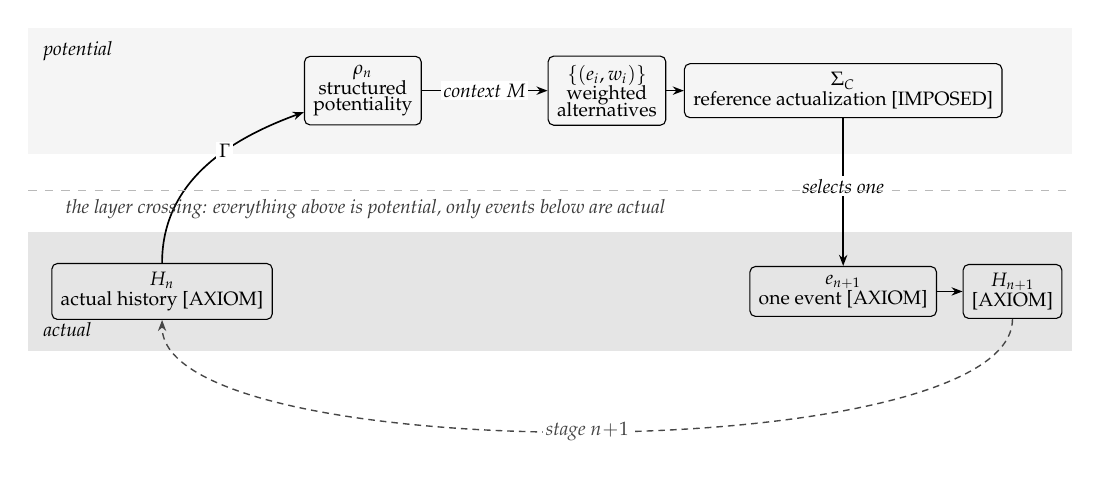
\begin{tikzpicture}
% --- the two ontological bands -------------------------------------
\begin{scope}[on background layer]
  \fill[black!4]  (-0.35,0.75) rectangle (12.9,2.35);
  \fill[black!10] (-0.35,-1.75) rectangle (12.9,-0.25);
\end{scope}
\node[font=\scriptsize\itshape, anchor=north west] at (-0.28,2.30)
  {potential};
\node[font=\scriptsize\itshape, anchor=south west] at (-0.28,-1.70)
  {actual};

% --- nodes ----------------------------------------------------------
\node[sel]   (H)   at (1.35,-1.0)  {$H_n$\\[-1pt]\figsub actual history [AXIOM]};
\node[sel]   (rho) at (3.9,1.55)   {$\rho_n$\\[-1pt]\figsub structured\\[-2pt]\figsub potentiality};
\node[sel]   (w)   at (7.0,1.55)   {$\{(e_i,w_i)\}$\\[-1pt]\figsub weighted\\[-2pt]\figsub alternatives};
\node[sel]   (S)   at (10.0,1.55)  {$\Sigma_C$\\[-1pt]\figsub reference actualization [IMPOSED]};
\node[sel]   (e)   at (10.0,-1.0)  {$e_{n+1}$\\[-1pt]\figsub one event [AXIOM]};
\node[sel]   (H1)  at (12.15,-1.0) {$H_{n+1}$\\[-1pt]\figsub [AXIOM]};

% --- flow -----------------------------------------------------------
\draw[con] (H) to[out=90,in=200] node[lbl,pos=0.62] {$\Gamma$} (rho);
\draw[con] (rho) -- node[lbl] {context $M$} (w);
\draw[con] (w) -- (S);
\draw[con] (S) -- node[lbl,pos=0.46] {selects one} (e);
\draw[con] (e) -- (H1);
\draw[wk] (H1) to[out=-90,in=-90,looseness=0.45]
  node[lbl,pos=0.5] {stage $n\!+\!1$} (H);

% --- the layer crossing --------------------------------------------
\draw[gray!55,dashed] (-0.35,0.28) -- (12.9,0.28);
\node[font=\figsub\itshape, anchor=west, gray!45!black] at (0.0,0.05)
  {the layer crossing: everything above is potential, only events below are actual};
\end{tikzpicture}
\caption{The shape of the recursion, drawn here before most of it has
been paid for. Structure is encoded in shape and rule, never in colour:
solid boxes are theorem-grade within their stated premises, while thin boxes
are axioms, selections, or imported representations. Actual history generates structured
potentiality through a state-assignment map $\Gamma$; a chosen context
resolves it into weighted alternatives; the actualization block selects
one; the record extends and the cycle repeats. Everything above the lower
band is potential; only the events in it are actual. \emph{Of the objects
shown, this section has bought only the two bands and the singular
event.} The state-assignment map, the context and the weights are
purchased in Section~\ref{sec:operational}, which is where the diagram
closes into the equation it depicts. The imposed $\Sigma_C$ closes only the
reference recursion; its physical substrate pushforward remains open.}
\label{fig:ontology}
\end{figure}

One thing this buys is worth isolating before going on, because it
is smaller than it looks. A record that extends has an order. What it
does not have is a scale on that order, and the next section shows why
that gap cannot be closed by looking at the record harder.

% =====================================================================
\section{Succession is not yet time}
\label{sec:succession}

What has been bought so far is a distinction and a rule for extending a
record. That is strictly less than a world, and the gap is worth naming
precisely, because it is the first place the construction has to spend.

Writing $H_{n+1} = H_n \circ e_{n+1}$ gives an \emph{order}. An order
supports two predicates, \emph{before} and \emph{after}, and it supports
nothing else. In particular it does not support \emph{how much}. Nothing
in a growing list distinguishes a long interval from a short one, because
the list has no second interval to compare against: each event is simply
the next.

A duration is a ratio. To say that one interval is $3.7$ of another is to
have counted something that happened $3.7$ times, so a unit is required
before a duration is meaningful, and a unit requires a \emph{recurrence}
--- a feature that comes back, so that returns can be counted. Monotone
succession never returns. Whatever supplies the recurrence is therefore
not the index; it is a physical thing inside the history, and it must be
paid for.

Two consequences follow, and they set up everything after this section.

First, the demand has a definite shape: a bounded degree of freedom, a
law that restores it, and a constant relating how far it swings to how
long it takes. That constant is where the price will show up, because the
restoring law is not free --- a substrate either supplies one or does not.

Second, and less obviously, the same argument applies to the paper's own
bookkeeping. The recursion this architecture will run on is indexed by the
ontic integer update order $n$. That index is a causal ordering variable,
not an elapsed duration. Operational duration requires a maintained local
clock with phase $\phi_x(n)$ and inferred duration $\tau_x$; actualization
introduces the still different count $k_x$ of phase-compliant gates. A clock
is therefore not a component of the architecture among others; it is a
precondition for turning update order into measured duration. That thread is
picked up in Section~\ref{sec:qg}, once there is a recursion on the page to
be indexed.

So: what is the cheapest recurrence a discrete substrate can host, what
constant does it keep, and what does it cost?

% =====================================================================
\section{Time: the clock}
\label{sec:clock}

Four questions, in the order Section~\ref{sec:succession} leaves them.
What does a period cost, in the sense of what fixes its constant? What
shapes can a substrate make available? Which of them, if any, is forced?
And what does the shortfall between those two answers cost, and buy? Each
subsection below answers exactly one of them.

\subsection{The setting}

The model is a discrete one: point bodies on a lattice, interacting
through a compact central pair potential with a single minimum at
separation $r_0$, and carrying a polarity that makes the interaction
graph bipartite. Two features matter. Every bond in an equilibrium sits
\emph{at} its potential minimum, so the configuration carries zero actual
tension; and the potential has compact support, so ``bonded'' is a sharp
predicate. What follows is exact within that model.

\subsection{What a period costs}
\label{sec:quadrature}

Before asking which oscillator a substrate supplies, it is worth asking
what the homogeneous power-law family charges. Take a symmetric confining potential
$V = \lambda|x|^n$ and release a body of mass $m$ from rest at amplitude
$A$, so $E = \lambda A^n$. Energy conservation fixes the speed,
$v = \sqrt{2(E-V)/m}$, and a quarter period is the time to cross from the
centre to the turning point:
\begin{equation}
\frac{T}{4} = \int_0^{A}\frac{\dd x}{v}
= A\sqrt{\frac{m}{2E}}\;I(n),
\qquad
I(n) = \int_0^1\frac{\dd u}{\sqrt{1-u^{n}}}
= \frac1n B\!\left(\tfrac1n,\tfrac12\right).
\label{eq:quadrature}
\end{equation}
Within this homogeneous family, everything specific to the clock is in
the $I(n)$ of \eqref{eq:quadrature}, and it factors into a square-root
quadrature term and a degree-dependent term:
\begin{equation}
I(n) \;=\; \underbrace{\sqrt{\pi}}_{\text{quadrature root}}
\;\cdot\;
\underbrace{\frac{\Gamma(1/n)}{n\,\Gamma(1/n+1/2)}}_{\text{degree ratio}} .
\label{eq:qrdr}
\end{equation}
The first factor is $\Gamma(\tfrac12)$, arising when the homogeneous
integral is reduced to a Beta function. The second factor is the part that
moves with the degree $n$. A generic mixed or nonhomogeneous potential has
no single degree and need not admit this factorization; $\sqrt\pi$ is not
claimed here as a universal charge of every mechanical clock.

\begin{center}
\small
\begin{tabular}{cccc}
\toprule
$n$ & $I(n)$ & degree ratio & \\
\midrule
$2$ & $1.5707963268$ & $0.8862269255$ & $=\sqrt\pi/2$ \\
$3$ & $1.4021821053$ & $0.7910965381$ & \\
$4$ & $1.3110287771$ & $0.7396687798$ & $=\Gstar/4$ \\
$5$ & $1.2537306248$ & $0.7073417591$ & \\
$6$ & $1.2143253239$ & $0.6851096988$ & \\
$8$ & $1.1635925712$ & $0.6564868082$ & \\
\bottomrule
\end{tabular}
\end{center}

Two rows are special, and their relation is the point.

At $n=2$ the degree ratio is $\Gamma(\tfrac12)/\Gamma(1) = \sqrt\pi/2$ ---
\emph{the quadrature root again}. The harmonic case is the unique
self-reproducing one, so its constant is $I(2) = \sqrt\pi\cdot\sqrt\pi/2 =
\pi/2$: a power of $\pi$ and nothing else. Within this family, the circle
constant in the harmonic row is therefore a Beta-function identity rather
than a separate geometric input.

At $n=4$ the degree ratio is $\Gstar/4$, giving $I(4) = \sqrt\pi\,\Gstar/4
= \varpi/2$, half the lemniscate constant. So $\pi$ and $\Gstar$ are not
rival constants competing to be fundamental. They are the same
quadrature factor multiplied by two different degree ratios, and
$\Gstar = 2\varpi/\sqrt\pi$ is that statement rearranged.

\subsection{A decidable trichotomy}

Let $R$ be the rigidity matrix of a framework, whose rows are the stretch
rates $\hat{u}_e\cdot(q_i-q_j)$ of each bond under a displacement field
$q$. Expanding a path $p(d) = p_0 + d\,q + d^2 w$, the stretch of bond $e$
is $d\,(Rq)_e + d^2[\kappa_e(q) + (Rw)_e] + O(d^3)$ with
$\kappa_e(q) = |q_i-q_j|_\perp^2/2\ell_e$. Three cases are exhaustive.

\begin{criterion}[The rigidity trichotomy]
\label{crit:trichotomy}
At zero tension, along a direction $q$:
\begin{enumerate}\itemsep2pt
\item if $Rq \neq 0$, the direction is first-order rigid and the energy
      grows as $d^2$: $n=2$, a harmonic clock;
\item if $Rq = 0$ and $\kappa(q) \perp \operatorname{coker} R$, the flex
      extends through second order; it may be obstructed at higher order
      or extend to a finite mechanism, so the quartic term vanishes and
      $n \ge 6$ or $n = \infty$;
\item if $Rq = 0$ but $\kappa(q)$ is not orthogonal to
      $\operatorname{coker} R$, the flex is \emph{blocked}, and minimizing
      over $w$ gives exactly
      \begin{equation}
      E(d) = \lambda(q)\,d^4 + O(d^5), \qquad
      \lambda(q) =
      \frac12\min_w\sum_e k_e\,[\kappa_e(q)+(Rw)_e]^2 >0 ,
      \label{eq:quartic}
      \end{equation}
      so $n=4$. If $\dim\operatorname{coker}R=1$, with generator
      $\hat\omega$, this reduces to
      $\lambda=\langle\hat\omega,\kappa\rangle^2/
      (2\sum_e\hat\omega_e^2/k_e)$; the minimum-viable carrier below has
      precisely this one-stress form.
\end{enumerate}
Hence $n=4$ at zero tension exists \emph{if and only if} a self-stress
exists and blocks the flex.
\end{criterion}

Two corollaries follow at once: no self-stress means no $n=4$, and actual
tension means $n=2$, since a nonzero equilibrium stress puts a $d^2$ term
on any flex it blocks. The quartic case lives only at the degenerate
point --- zero actual tension with nonzero \emph{possible} stress. This
makes what is otherwise a question about potential shapes decidable by
linear algebra.

The trichotomy matters because the three cases keep time differently
(Figure~\ref{fig:trichotomy}). The harmonic case is isochronous and its
quadrature contains $\pi$, which \eqref{eq:qrdr} has already explained.
The quartic case is the anti-pendulum: its frequency grows with
amplitude, and its period law contains the lemniscatic ratio
\begin{equation}
\Gstar = \frac{\Gamma(\tfrac14)}{\Gamma(\tfrac34)} = 2.958675119188639\ldots
\end{equation}

\begin{figure}[t]
\centering
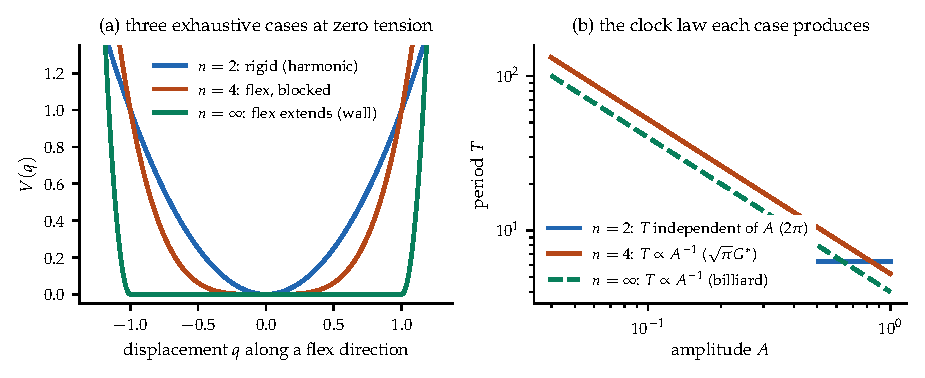
\includegraphics[width=\textwidth]{trichotomy.pdf}
\caption{The rigidity trichotomy and the clocks it produces. (a) The three
exhaustive cases of Criterion~\ref{crit:trichotomy} at zero tension.
(b) The corresponding period laws for the plotted normalization
$m=1$, $V=|x|^n/2$: the harmonic coefficient is $2\pi$; the quartic
coefficient is $\sqrt\pi\,\Gstar$ in $T\propto A^{-1}$; a hard wall also
gives $T\propto A^{-1}$ but with no special coefficient.}
\label{fig:trichotomy}
\end{figure}

\subsection{What forces the quartic, and what does not}
\label{sec:threshold}

The trichotomy says a quartic clock is \emph{available}. A stronger
statement is available too, and because it is the one most likely to be
over-read, it is stated with its hypotheses attached and its failure
modes named.\footnote{The reading of the quartic as the clock of marginal
stability, together with the period law and the anti-pendulum framing,
originates in a companion manuscript on the edge-of-stability clock; what
is added here is the statement as a proposition with named hypotheses,
the factorisation \eqref{eq:qrdr}, and the finite-amplitude term.}

\begin{proposition}[Threshold forcing]
\label{prop:threshold}
Let a single degree of freedom evolve in a potential $V(x;\mu)$ such that
\begin{enumerate}\itemsep2pt
\item[\textnormal{(H1)}] $V$ is smooth in $x$ and in a control parameter
  $\mu$, with one degree of freedom;
\item[\textnormal{(H2)}] $V$ is invariant under $x\mapsto-x$;
\item[\textnormal{(H3)}] the family crosses $\mu=0$ transversally, at
  which point $\partial_x^2V(0;0)=0$;
\item[\textnormal{(H4)}] the quartic coefficient is nonzero,
  $\lambda \equiv \tfrac1{4!}\partial_x^4V(0;0) > 0$.
\end{enumerate}
Then at $\mu=0$ the leading behaviour is $V = \lambda x^4 + O(x^6)$, and
\emph{in the limit $A\to0$}
\[
T\cdot A \;=\; \sqrt{\pi}\,\Gstar\sqrt{m/2\lambda}.
\]
\end{proposition}

The content is in what each hypothesis excludes. (H2) is what kills the
cubic --- and it kills it \emph{by symmetry, not by tuning}, which is why
the quartic is generic here rather than fine-tuned. (H3) is the
threshold. (H4) is nondegeneracy. And the $A\to0$ clause is not
decoration: it is the whole of the second failure mode below.

\paragraph{The substrate is not known to sit at a threshold.}
Proposition~\ref{prop:threshold} forces the quartic \emph{given} a
threshold; it says nothing about why a substrate would be at one. Since
$\mu=0$ is a codimension-one surface, the generic configuration is not on
it, and staying on it is a condition that must be actively held. The
price is therefore a maintenance cost paid continuously, not a
construction cost paid once --- which is the sense in which this is a
clock at the \emph{edge} of stability rather than a clock in a well.

\paragraph{Two ways it fails, and only one of them is obvious.}
Dropping (H4) entirely gives a pure sextic and a single different
constant, $4I(6)/\sqrt\pi = 2.7404387952$. That failure is visible.

The other is not, and it is a genuine counterexample to any
finite-amplitude version of the proposition. Take $V = \lambda x^4 + \nu
x^6$ with both terms present, and write $r = \nu A^2/\lambda$. Then
\begin{equation}
T\cdot A = 4\sqrt{\frac{m}{2\lambda}}
\int_0^1\frac{\dd u}{\sqrt{(1-u^4) + r\,(1-u^6)}},
\label{eq:sexticdrift}
\end{equation}
and the constant sweeps \emph{continuously} with $r$: the bracket runs
$5.2441$, $5.2133$, $4.9589$, $3.5563$ at $r = 0,\,0.01,\,0.1,\,1$. Every
member of this family has $\lambda\neq0$, so (H4) does not exclude it.
What excludes it is the limit: $r\propto A^2$, so the drift vanishes
with the amplitude and $\Gstar$ is the $A\to0$ endpoint, not a
finite-amplitude value.

It is tempting to read this paper's own measurement as the same term, and
an earlier draft did. That reading was wrong twice over, and the
correction is worth more than the coincidence was. The exploratory
twelve-degree-of-freedom \emph{harmonic-bond surrogate} of
Section~\ref{sec:mvc} holds
$T\cdot A$ constant only to $0.33\%$ across a sixfold amplitude range,
recovering $\Gstar$ to $2\times10^{-6}$ only in the $A\to0$
extrapolation. But that $0.33\%$ is an \emph{excess}, not a deficit:
$T\cdot A$ \emph{rises} with amplitude and every recovered $\Gstar$ sits
\emph{above} $\Gstar$, which in the coordinates of
\eqref{eq:sexticdrift} is $r<0$, not $r>0$. And the excess is not mostly
the sextic term at all --- Section~\ref{sec:mvc} decomposes it, and
$22.7$ parts in $23$ are \emph{kinetic}, a correction this family does not
contain. The drift and the counterexample family are \textbf{not} one
term seen twice. They are two different terms of comparable size, and
only the smaller one belongs to this section.

\subsection{Off the threshold, exactly}
\label{sec:crossover}

The proposition holds \emph{at} $\mu = 0$. Since the whole price is that
$\mu = 0$ must be held, what happens as it slips is not a footnote --- it
is the thing being paid for, and it is exactly solvable.

For the normal form $V = \tfrac12\mu x^2 + \lambda x^4$ the quadrature
closes in elliptic functions: the orbit is $x(t) = A\,\mathrm{cn}(\Omega
t;\kappa)$ with $\Omega^2 = (\mu+4\lambda A^2)/m$, and writing everything
in terms of the modulus
\begin{equation}
\kappa^2 = \frac{2\lambda A^2}{\mu + 4\lambda A^2}
\label{eq:modulus}
\end{equation}
eliminates $\mu$ and $A$ separately, leaving a single universal curve:
\begin{equation}
\boxed{\;T\,A\,\sqrt{\tfrac{2\lambda}{m}} \;=\; 4\,\kappa\,K(\kappa)\;}
\label{eq:collapse}
\end{equation}
with $K$ the complete elliptic integral of the first kind. Every
origin-crossing oscillation (and, for $\mu<0$, every over-barrier
oscillation) lies on this one curve: the harmonic side
at $\kappa^2\to0$, the double-well side at $\tfrac12<\kappa^2<1$, and the
quartic clock at exactly $\kappa^2 = \tfrac12$, where
$4\kappa K = \sqrt\pi\,\Gstar$ and \eqref{eq:periodlaw} is recovered.

Two things follow, and the second is the more interesting.

\emph{The threshold is a self-dual point.} $\kappa = 1/\sqrt2$ is the
fixed point of the exchange $\kappa\leftrightarrow\kappa'$ between a
modulus and its complement, where $K' = K$. So $\Gstar$ is not merely the
constant of one potential among many; it is the value the period takes at
the one modulus that is its own complement. This is a distinct
self-duality: the quartic threshold lands on the complementary-modulus
fixed point $\kappa^2=1/2$, whereas Section~\ref{sec:quadrature}'s harmonic
self-reproduction is the recurrence of $\Gamma(1/2)=\sqrt\pi$. Both are
fixed-point structures, but they are not the same identity.

\emph{The constant drifts two ways, and both are now exact.} Detuning
moves $\kappa^2$ off $\tfrac12$ along \eqref{eq:collapse}; a sextic
admixture moves the constant along \eqref{eq:sexticdrift} in $r$. They
are independent perturbations --- one changes the quadratic coefficient,
the other adds a higher one --- and $\Gstar$ is the corner $s\to0$,
$r\to0$ of the reduced plane, where $s = \mu/2\lambda A^2$ and
$r = \nu A^2/\lambda$.

\emph{The rate matters, and this is sharper than a double limit.} Read
back in the bare parameters, $\mu\to0$ and $A\to0$ \emph{together do not
suffice}: the reduced detuning $s$ is a ratio, so the value attained
depends on the path. Sending $\mu\to0$ with $\mu/A^2$ held at any nonzero
constant leaves $s$ fixed and returns $4\kappa K(\kappa)$ at that
modulus, not $\sqrt\pi\,\Gstar$; taking $A\to0$ first at fixed $\mu$
sends $s\to\infty$ and the constant to zero. Even the two iterated limits
disagree. The condition that selects the lemniscatic value is
$\mu/A^2\to0$ --- the detuning must vanish \emph{faster than the
amplitude squared}. This is the price stated exactly: $\Gstar$ is not
merely a corner but a corner approached at a controlled rate.
Figure~\ref{fig:collapse} draws both statements at once: the one curve
every detuning lies on, and the two-drift plane whose corner is the only
point where the constant lives.

\begin{figure}[t]
\centering
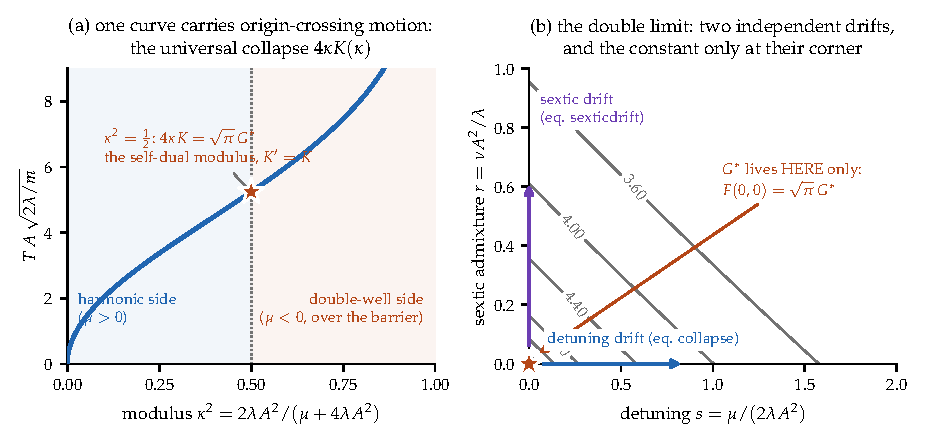
\includegraphics[width=\textwidth]{collapse.pdf}
\caption{The crossover, exactly, and the double limit. (a) Every
origin-crossing oscillation of the normal form (including over-barrier
motion for $\mu<0$) lies on the single curve
$T A\sqrt{2\lambda/m} = 4\kappa K(\kappa)$: harmonic side as
$\kappa^2\to0$, oscillation over the double-well barrier for
$\kappa^2>\tfrac12$, and the quartic clock at exactly $\kappa^2 =
\tfrac12$ --- the self-dual modulus $K'=K$ --- where the value is
$\sqrt\pi\,\Gstar = 5.2441$. (b) The two drift directions are
independent: detuning $s$ moves the constant along
\eqref{eq:collapse}, sextic admixture $r$ moves it along
\eqref{eq:sexticdrift}, and $\Gstar$ is attained only at the corner
$(0,0)$ of \emph{these reduced} coordinates. In the bare parameters that
corner requires $\mu/A^2\to0$, not merely $\mu\to0$ and $A\to0$: a path
holding $\mu/A^2$ fixed runs along a horizontal line of the plane and
never reaches the corner. Contours are exact quadrature; the corner value
agrees with $\sqrt\pi\,\Gstar$ to $10^{-9}$.}
\label{fig:collapse}
\end{figure}

\subsection{The native screen finds no quartic clock}
\label{sec:native}

Which cases does the model realize by itself? Its zero-tension equilibria
are exactly the frameworks whose active bonds all sit at $r_0$ with
opposite-polarity endpoints --- unit-edge bipartite frameworks. A screen
over every connected minimum-degree-two bipartite interaction graph up to
$N=7$, plus the cube graph, found \textbf{no self-stressed embedding}:
seventeen graph classes, zero hits, with constraint-clean minima of
$\lambda_{\min}(RR^{\mathsf T})$ bounded away from zero at $1.03\times
10^{-2}$. Exactly, the cubic checkerboard blocks at $L=2,3,4$ have
self-stress dimension zero, so all their flexes extend. Larger stressed
objects contract to networks of straight unit chains meeting at joints,
and the two minimal joint graphs are squeezed by geometry: an interior
four-joint configuration has a joint angle of at most $30^\circ$ against
a clearance requirement of $28.96^\circ$, and an exhaustive
integer-distance search --- 153{,}898 integral quadruples to diameter 60,
7{,}177 of them with an interior point --- tops out at $26.14^\circ$.

One object survives the static gates: a nineteen-body hexagonal wheel,
all twenty-four bonds exactly unit, with a one-dimensional equilibrium
self-stress certificate (positive signs on the rim, negative signs on the
spokes; not an applied force) and every individual chain-bowing
flex blocked. It is, to our knowledge, the first zero-tension
self-stressed equilibrium exhibited in this model. \emph{And it fails as
a clock.} Its quartic form is a squared difference,
$E_4 \propto (\sum\kappa_{\rm rim} - \sum\kappa_{\rm spoke})^2$, so the
combined flex that bows the rim and buckles the spokes equally costs
nothing: the blocking form on the 28-dimensional nontrivial flex space is
sign-indefinite, with eigenvalues from $-1.467$ to $+0.743$. Direct
integration confirms it, the constrained static energy collapsing to
$\sim10^{-12}$. The verified per-chain quartic was a chord across a flat
valley.

The failure sharpens the criterion, and the sharpened form is a genuine
result of this paper:

\begin{criterion}[Buckling]
\label{crit:buckling}
Chain stations are free hinges, so a \emph{compressed} chain of length
$\ge 2$ buckles at zero energy; only tensioned chains are
straight-stable. A native $n=4$ clock therefore requires, beyond
Criterion~\ref{crit:trichotomy}: \textup{(1)} a self-stress;
\textup{(2)} a blocking form definite on the \emph{whole} flex space, not
merely mode by mode; and \textup{(3)} every compressed member a
\emph{single bond}.
\end{criterion}

Because an all-tension self-stress is impossible on a finite framework,
condition~(3) forces mixed structures --- single-bond struts together
with straight tensioned chains. Whether such an integer ``unit-strut
tensegrity'' exists in this model is open; the first candidate family is
killed exactly, its closure condition $s^2-4k^2=-1$ being impossible
modulo~4.

\subsection{The minimum viable clock}
\label{sec:mvc}

Given the native screen's null, what is the cheapest purchased object whose
leading soft mode realizes it? The minimal construction and its
$A\to0$ normal form are exact. Take four bodies $A^+B^-C^+D^-$
collinear at positions $0,1,2,3$, with the three unit bonds at their
minimum (curvature $k_1$) and \emph{one additional interaction species}
closing $A$ to $D$ at its own minimum at range $3r_0$ (curvature $k_2$).
All four bonds are at zero tension. Then $\operatorname{rank}R = 3$, the
self-stress is one-dimensional with $\omega=(1,1,1,-1)$, and the blocking
form for each transverse axis has profile spectrum
$\{0,0,2,10/3\}$, whose kernel is translation plus rigid rotation. After
quotienting those trivial motions and including both transverse axes, the
four-dimensional nontrivial flex space has spectrum
$\{2,2,10/3,10/3\}$ and zero kernel --- positive definite on
\emph{every} nontrivial flex. The chain is second-order rigid at zero
actual tension, certified by this positive self-stress form: $n=4$ in
every nontrivial infinitesimal-flex direction (longitudinal stretch
directions remain quadratic). Crucially the certificate's one compressive
member is a single bond, so Criterion~\ref{crit:buckling} is satisfied where the wheel
failed.

The mirror-even zero-momentum mode $q = (-1,+1,+1,-1)U$ is transverse, so
it elongates the outer bonds only at \emph{second} order and the chain
relaxes longitudinally in response. Together with the two longitudinal
stretches it drives, it spans a dynamically invariant
\emph{three}-degree-of-freedom sector; adiabatically eliminating the two
stiff stretches closes it as a one-degree-of-freedom oscillator that is
purely quartic in the $A\to0$ limit --- an instance of
\eqref{eq:quartic}, with the blocked-flex coefficient evaluated on this
stress --- with
\begin{equation}
\lambda_{\rm eff} = \frac{8k_1k_2}{k_1+3k_2}, \qquad m_{\rm eff} = 4,
\qquad
\boxed{\;\lim_{A\to0}T\cdot A = \sqrt{\pi}\,\Gstar\,
\sqrt{\frac{m_{\rm eff}}{2\lambda_{\rm eff}}}
= \sqrt{\pi}\,\Gstar\,\frac{\sqrt{k_1+3k_2}}{2\sqrt{k_1k_2}}\;}
\label{eq:periodlaw}
\end{equation}
Direct integration of the ideal quartic normal form reproduces
\eqref{eq:periodlaw} to machine precision. Separately, an exploratory
twelve-degree-of-freedom conservative \emph{harmonic-spring surrogate}
matched only at the stated curvatures holds $T\cdot A$ constant to $0.33\%$
across a sixfold amplitude range, recovering $\Gstar$ to $2\times10^{-6}$
in the $A\to0$ extrapolation \emph{with no fitted scale}
(Figure~\ref{fig:clock}).

\emph{And the surrogate residual is computable, which is better than calling it
small.} Relaxing the harmonic-spring chain at fixed $U$ gives a reduced system that is
not the ideal normal form in two respects. Its potential carries a sixth
order term,
\[
\begin{aligned}
E_{\rm eff}(U)={}&\lambda_{\rm eff}U^4 \\
&+\frac{16k_1k_2(k_1-k_2)}{(k_1+3k_2)^2}U^6+\cdots ,
\end{aligned}
\]
which vanishes
\emph{only} at equal couplings --- where the series runs
$2U^4 - 2U^8 + 6U^{12}$, in powers of four alone --- so the equal-coupling
purity is a cancellation, not a law. And its reduced \emph{mass} is
amplitude dependent, $m_{\rm eff}(U) = 4 + 4U^2 - \cdots$, a correction
the sextic family of Section~\ref{sec:crossover} does not contain at all.
Quadrature on that surrogate reduction reproduces the simulated drift
($+0.328\%$ against $+0.331\%$ at $A=0.12$) and decomposes it:
$+0.314\%$ kinetic against $+0.014\%$ potential, a ratio of $22.7$. The
drift is therefore an \emph{excess}, dominated by the mass term --- which
is why it is not the sextic admixture of Section~\ref{sec:crossover}, and
why $\Gstar$ is recovered only in the limit where both corrections
vanish.

Minimality is exact by enumeration: at $N\le3$ the opposite-polarity
graphs are trees and cannot carry stress; at $N=4$ the single-scale
embeddings have no stressed realization; and polarity alternation forces
the closure span to be odd, hence $3r_0$ at minimum. \textbf{Four bodies
and one additional interaction range is the floor.}

Two remarks about $\omega = (1,1,1,-1)$, since the sign pattern invites a
reading it will not support. It is indexed by \emph{bonds}, not
directions, and its signs denote tension/compression capacity in an
equilibrium self-stress certificate, not actual force at the potential
minima: the lone minus
sits on the closure bond, forced both by the impossibility of an
all-tension self-stress on a finite framework and by a four-cycle having
exactly one closure. The object that could carry a signature is the
blocking form, whose coefficients these are --- and it is positive
\emph{semi}-definite, spectrum $\{0,0,2,10/3\}$, with no negative
direction at all. Written in the consecutive stretches $u_i$ it is
$\propto 3\sum u_i^2 - (\sum u_i)^2$, the variance: the minus subtracts a
mean and thereby removes the rigid-motion zero mode. It does not open a
cone. An \emph{indefinite} blocking form is precisely a buckling mode,
which is how the wheel of Section~\ref{sec:native} failed.

\paragraph{And the carrier cannot test what it was built beside.}
Recorded here, at the point of purchase, rather than where it is later
needed: this clock is a mechanical framework, $m\ddot q = -\nabla
V(|q_i-q_j|)$, and such an equation is \emph{Galilean} invariant.
Boosting it leaves the period exactly unchanged at any velocity, so it
would report zero time dilation whatever the substrate did. The carrier
is therefore disqualified as an instrument for the relativistic
obligations of Section~\ref{sec:relativity} --- not by a defect in its
construction, but by the kind of object it is.

\begin{figure}[t]
\centering
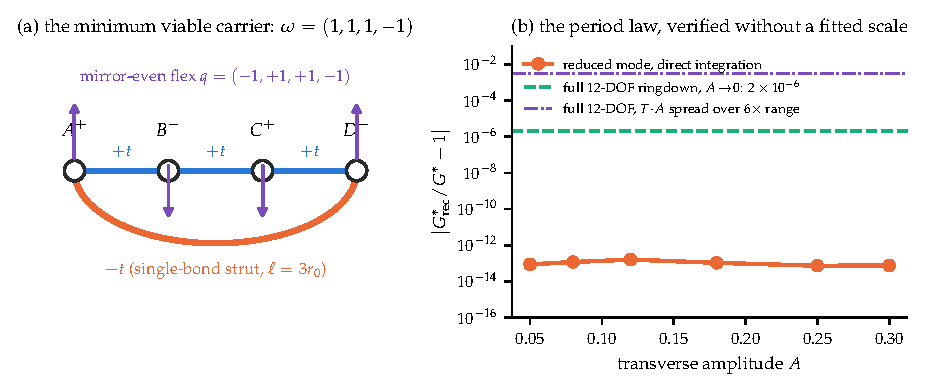
\includegraphics[width=\textwidth]{clock.pdf}
\caption{The minimum viable leading-order quartic clock carrier. (a) Four
bodies, three unit bonds and one single-bond closure at range $3r_0$.
The signs of $\omega=(1,1,1,-1)$ encode the possible equilibrium
self-stress, not actual forces; the blocking form is positive definite on
every nontrivial flex, so the unstressed framework is second-order rigid.
(b) The $A\to0$ period
law~\eqref{eq:periodlaw} verified without a fitted scale: direct
integration of the ideal quartic normal form reproduces it to machine
precision, while the two horizontal lines mark the independent
twelve-degree-of-freedom harmonic-spring surrogate and its finite-amplitude
drift. They are not a simulation of the registered compact bond law.}
\label{fig:clock}
\end{figure}

\begin{scopebox}
\textbf{The price.} One additional interaction species, plus its scale
parameters. What it buys exactly is a quartic leading normal form and the
minimal four-body construction; the declared carrier is guaranteed only
through its asymptotic normal form, and its compact-law finite-amplitude
motion has not been simulated. Nor does the purchase by itself establish
a spectral window. In the curvature-normalized harmonic surrogate used
for the screen, $k_1=k_2=k$ and clearing the propagating band requires
$kA_{\max}^2>1.0556$, or $k>4.22$ at $A_{\max}=0.5$. This number is not a
compact-law depth bound: the registered unit bond has
$k_1=96\varepsilon$ and a same-shape range-three closure has
$k_2=(32/3)\varepsilon_2$, so the conversion depends on the additional
ratio $\rho$. A compact-law dynamical screen remains to be run. The
carrier's true price therefore includes matter stiffness at
field-stiffness parity. Its falsifier is stated in
Appendix~\ref{app:instruments}.
\end{scopebox}

\subsection{What the lemniscatic price buys}
\label{sec:gstarprice}

The price is now fully stated: one interaction species, and a threshold
that must be held. What has not been stated is what it returns. A ledger
that records a cost and not its purchase is an unstable thing to leave
standing, and the structure of the last three subsections settles it.

Read the table of \eqref{eq:qrdr} again, this time as a list of
degeneracies. Only $n=2$ has nonzero second-order stiffness; every
$n\ge4$ is second-order \emph{free} and still oscillates. Ordinarily
those properties exclude one another --- a stiff mode oscillates but
resists being moved, a soft mode moves freely but does not oscillate ---
and the quartic is the \emph{minimal} escape, needing exactly one
vanishing Taylor coefficient where $n=6$ needs two. $\Gstar$ is the period
constant of that minimal degeneracy.

The purchase is then exact. Fixing mass, displacement and period, the
energy to hold the mode displaced is
\begin{equation}
\frac{E\,T^2}{mA^2} = 2\pi^2 \ \ \text{(harmonic)}, \qquad
\frac{\pi}{2}G^{*2} \ \ \text{(quartic)}, \qquad
\frac{E_{\rm quartic}}{E_{\rm harmonic}} = \frac{G^{*2}}{4\pi} = 0.6966,
\label{eq:gstarprice}
\end{equation}
the stiffness cancelling from both, so the ratio is pure $G^*$. And at
displacement $a$ the ratio is $(a/A)^2 G^{*2}/4\pi$, which vanishes: a
degenerate direction is free to first order, so at a tenth of the
reference displacement the quartic mode is $144$ times cheaper to move.
Figure~\ref{fig:clockgeometry} sets the two clocks beside each other ---
their constants as arc lengths, their orbits at equal energy, and the
threshold surface on which the quartic one lives.

\begin{figure}[p]
\centering
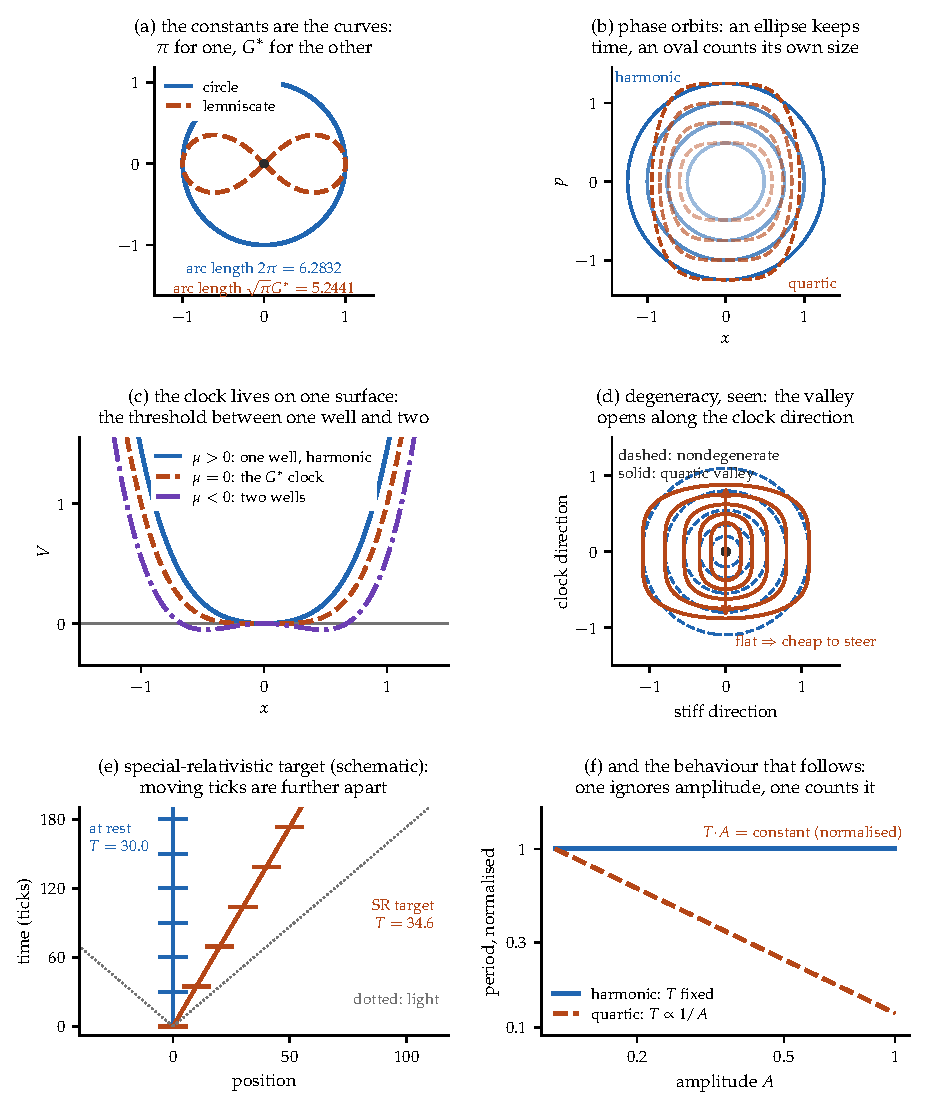
\includegraphics[width=0.98\textwidth]{clockgeometry.pdf}
\caption{The two clocks, seen. (a) The constants are not normalisations
but arc lengths: the unit circle's is $2\pi = 6.2832$, the unit
lemniscate's is $\sqrt\pi G^* = 5.2441$ --- the latter integrated
numerically here and agreeing with $B(\tfrac14,\tfrac12)$ to $10^{-7}$.
(b) Phase orbits at equal energy steps: harmonic level sets are ellipses
traversed uniformly, so the period ignores the orbit's size; quartic ones
are flat-flanked ovals and are traversed faster as they grow. (c) The
degenerate clock does not live at a generic point but on a single surface
--- the threshold $\mu = 0$ between one well and two, where the cubic is
forbidden by symmetry and the quartic is what remains. This is the
picture of Proposition~\ref{prop:threshold}: the codimension-one surface
is the hypothesis, and being off it is the generic case. (d) The degeneracy
made visible: contours about a nondegenerate minimum are closed ellipses
(dashed), while the quartic valley (solid) opens along the clock
direction. That flatness is the cheapness of \eqref{eq:gstarprice}.
(e) The special-relativistic dilation target as a schematic: tick events
on two worldlines, one at rest and one at $u=0.5\,C$, with the moving
ticks separated by $\gamma$. This panel contains no soliton shape-mode
measurement; that campaign is classified as unreproduced in
Section~\ref{sec:oneenergy}.
(f) The behaviour that follows.}
\label{fig:clockgeometry}
\end{figure}

Proposition~\ref{prop:threshold} located the genericity, and it is worth
saying what that buys as well as what it costs. The quartic clock is the
normal form of a perfect Euler column at critical load and of any
mean-field symmetry-breaking order parameter; what is non-generic about
it is not the shape of the potential but the \emph{location}.

\paragraph{Why the maintenance is expensive, and not merely required.}
There is a sharper reason than codimension, and it is the same fact that
made horology choose $n = 2$. A clock whose frequency tracks its own
amplitude converts every amplitude perturbation into a frequency
perturbation. Isochronism is not an aesthetic preference but \emph{noise
immunity}: the pendulum's $\partial T/\partial A \approx 0$ is the whole
reason clocks work, and the anti-pendulum maximises exactly the coupling
the pendulum was chosen to suppress. Near threshold the mode is soft,
susceptibilities grow and relaxation slows --- so the very sensitivity
that makes critical points interesting makes them poor timekeepers.

That inverts usefully. A defect of a clock is a virtue of a sensor, and
what this oscillator's timing is exquisitely sensitive to is
\emph{its own distance from the threshold}: by \eqref{eq:collapse} the
measured $(T,A)$ pair fixes $\kappa$, and by \eqref{eq:modulus} $\kappa$
is the order parameter of the detuning. So a marginal clock reads out the quantity it must hold
fixed. The v2 reference construction closes this as a control problem by
selection: one context-blind feedback channel drives the dimensionless
detuning $\delta=\mu/A^2$ toward zero, while a second stabilizes amplitude
or action. Its audit records controller work, dissipation, detuning, and
amplitude; maintenance is never treated as free. A gate opens only at a
fixed phase crossing and under preregistered compliance tolerances. This
constructs a mathematical controller, not a native substrate actuator.
Figure~\ref{fig:sensorloop} separates the implemented reference loop from
that remaining physical debt.

\begin{figure}[t]
\centering
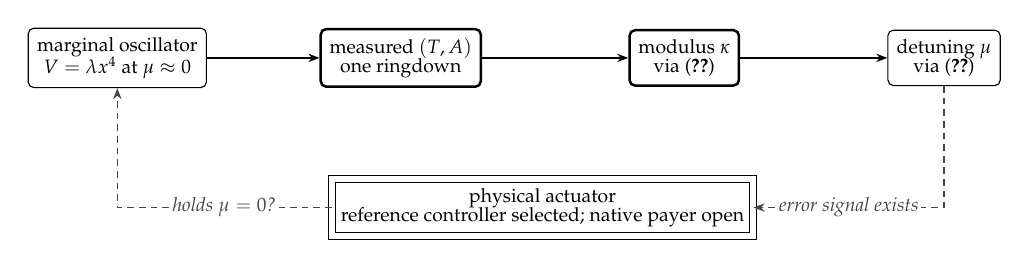
\begin{tikzpicture}
\node[sel]   (osc) at (0,0)     {marginal oscillator\\[-1pt]\figsub $V=\lambda x^4$ at $\mu\approx0$};
\node[thm]   (ta)  at (3.6,0)   {measured $(T,A)$\\[-1pt]\figsub one ringdown};
\node[thm]   (kap) at (7.2,0)   {modulus $\kappa$\\[-1pt]\figsub via \eqref{eq:collapse}};
\node[sel]   (mu)  at (10.5,0)  {detuning $\mu$\\[-1pt]\figsub via \eqref{eq:modulus}};
\node[openb] (act) at (5.4,-1.9) {physical actuator\\[-1pt]\figsub reference controller selected; native payer open};
\draw[con] (osc) -- (ta);
\draw[con] (ta) -- (kap);
\draw[con] (kap) -- (mu);
\draw[wk]  (mu) |- node[lbl,pos=0.75] {error signal exists} (act);
\draw[wk]  (act) -| node[lbl,pos=0.25] {holds $\mu=0$?} (osc);
\end{tikzpicture}
\caption{The sensor inversion and its status split. A marginal clock's
timing fixes its own distance from the threshold --- the solid path is
exact --- so the error signal needed to hold $\mu=0$ demonstrably exists.
The v2 reference controller consumes that signal with context-blind dual
feedback and audits its work and dissipation. The double-ruled block is the
still-missing native actuator: reference stabilization is not evidence that
the substrate pays the maintenance cost.}
\label{fig:sensorloop}
\end{figure}

So the price is a maintenance cost, continuously paid, not a construction
cost; and \eqref{eq:gstarprice} is what it returns. \emph{$\pi$ is native
because sitting off the threshold is generic; $G^*$ is priced because
sitting on it must be actively held} --- and what the holding buys is that
timekeeping and steerability stop trading against each other. A carrier
required only to be stable will be harmonic, since stability alone selects
a point off the threshold; a carrier that must also be reconfigurable at
low cost is pushed onto it.

This is also where the agency reading acquires a mechanism rather than an
analogy. An agent, thermodynamically, is a system that spends free energy
to hold a configuration against drift --- and holding $\mu = 0$ is exactly
that: an unmaintained system falls off the threshold and becomes a
harmonic clock. The sharp form of the question is therefore not whether
agents keep lemniscatic time, but that \emph{a $G^*$ clock is one which
must be actively maintained, and what the maintenance buys is cheap
actuation}. That is a claim about control cost. It neither requires nor
supplies anything about consciousness, and marginal stability --- a
genuine hallmark of adaptive systems --- is equally a property of sandpiles
and buckling columns.

\begin{scopebox}
\textbf{This interprets $G^*$; it does not recover it.} The proposition
forces the quartic \emph{given} a threshold, a reflection symmetry and a
nonvanishing quartic coefficient. Nothing here forces a substrate to sit
at a threshold, and \textbf{no valid carrier has produced $G^*$}: the
native single-scale screen returned zero, the four-body carrier that does
produce it needs a purchased interaction species and is Galilean and
therefore disqualified as a relativistic instrument. The only positive
dilation fit reported here is isochronous --- a $\pi$-clock --- and uses a
fitted speed about six percent below the free-sector energy speed, so it
does not establish a shared relativistic clock.
$G^*$ enters this framework by choice. Its selected role is purely temporal:
it controls when a compliant event is eligible, while $\Sigma$ controls which
outcome occurs. Conflating those two roles would make the Born argument
circular. Nor does the argument reach
agency: it is a selection statement about efficient design, and marginal
stability, while a hallmark of adaptive systems, is equally a property of
sandpiles and buckling columns.
\end{scopebox}

\subsection{What a clock is owed by the rest of the paper}

One forward debt is worth naming before leaving. The recursion this
architecture runs on is indexed by a stage, and an index is not a
duration: something physical has to carry it. That makes the clock not a
subplot of the architecture but a precondition of its own bookkeeping.
Section~\ref{sec:qg} pays this out, once there is a recursion on the page
to be indexed.

A clock, though, is not yet a record. One that is reset by every
fluctuation counts nothing, because counting requires that the last tick
still be there when the next arrives. Persistence is a separate purchase
and it is made in the same currency --- an energy barrier --- which is the
subject of the next section.


% =====================================================================
\section{Memory: the register}
\label{sec:register}

A clock alone carries no past. The minimal memory in the same model is a
single body cradled by three anchors on an equilateral triangle of side
$s<\sqrt3$: for such $s$ there are two mirror equilibria at heights
$\pm h$, $h = \sqrt{1-s^2/3}$, with all three bonds at exactly $r_0$.
The registered compact bond law is a polynomial in the squared normalized
distance $q=(r/r_0)^2$:
\begin{equation}
V(q) =
\begin{cases}
-16\varepsilon(q-\tfrac32)^2(q-\tfrac34), & q<\tfrac32,\\
0, & q\ge\tfrac32.
\end{cases}
\label{eq:registerbond}
\end{equation}
It has $V(1)=-\varepsilon$ and radial curvature
$\dd^2V(r^2)/\dd r^2|_{r=1}=96\varepsilon$.

The barrier between them is not a fitted quantity, and it is not a
measurement either. An explicit hinge path --- break one bond, swing on
the remaining two --- costs exactly $1.000\,\varepsilon$, which bounds it
above. The matching lower bound needs no grid over most of its domain.

\begin{proposition}[Register barrier]
\label{prop:registerbarrier}
For $s\in[0.9,1.3]$ the register's barrier is exactly one bond's
dissociation depth, independent of the geometry: $\Delta E = \varepsilon$,
and the minimax level is attained by an in-plane two-bond configuration,
one of the symmetry-related hinge crossings.
\end{proposition}

\begin{proof}[Proof sketch]
The two minima sit at $z=\pm h$, so any continuous path between them has
a moment with $z=0$: \emph{every} path crosses the anchor plane. Hence
$\Delta E \ge \min_{z=0}E - E_{\rm ground}$, which replaces a min--max
over paths by a minimisation over a plane. On that plane write $N$ for
the number of bonds whose squared distance lies in the attractive window
$q\in(3/4,\,3/2)$. The bond
law satisfies $V\ge-\varepsilon$ everywhere, $V\ge0$ for $q\le3/4$, and
--- decisively --- $V\equiv0$ for $q\ge3/2$. So $E\ge-\varepsilon N$
pointwise, and wherever $N\le2$ we have $E\ge-2\varepsilon$. Outward-rounded
interval arithmetic over boxes in $(x,y,s)$ brackets every squared bond
distance $q=d^2$ over the whole box. Over
$11{,}250{,}000$ closed boxes on an exact rational partition of
$(x,y,s)\in[-3/2,3/2]^2\times[9/10,13/10]$, every box has $N\le2$;
there are zero three-attractive candidates and zero uncertified boxes.
Every binary64 primitive is widened by one ULP with
\texttt{nextafter}. Outside the square the origin bond has
$q\ge9/4>3/2$, so the exact $N\le2$ argument covers the rest of the
infinite plane. No point samples or potential-energy fallback bounds enter
the certificate. The value
$-2\varepsilon$ is attained: in-plane the
body sits at distance exactly $r_0$ from two anchors, its distance to the
third being $d_3(s)=s\sqrt3/2+\sqrt{1-s^2/4}$. Analytically,
$d_3'(s)>0$ whenever $s^2<3$, and
$d_3(9/10)>323/200>3/2$, hence $q_3=d_3^2>3/2$; the third bond contributes exactly zero
throughout the interval. With $E_{\rm ground}=-3\varepsilon$ this gives
$\Delta E\ge\varepsilon$, and the hinge path gives
$\Delta E\le\varepsilon$.
\end{proof}

Two holes in an earlier version of this certificate are worth recording,
both found by review. It sampled five values of $s$ rather than the
interval and, more fundamentally, treated Euclidean distance $d$ as the
polynomial variable $q=d^2$. At $s=1.3$ it compared the centroid distance
$d=0.75056$ with the squared-distance window edge $q=3/4$, inventing a
three-attractive pocket; the correct centroid value is
$q=s^2/3=0.56333\ldots<3/4$, so no such pocket exists. Exact rational box
coverage plus outward-rounded bounds on $q=d^2$ remove both errors. The
certificate is machine-readable under schema
\texttt{ftd.register\_barrier.interval-certificate.v1}.

Compact support is load-bearing here, and worth naming as the modelling
choice it is: under a Morse or Lennard-Jones tail the third bond would
contribute a small negative amount at the crossing and the barrier would
sit strictly \emph{below} $\varepsilon$. The earlier watershed
computation, which returned $1.016$--$1.021\,\varepsilon$, is now
diagnosed rather than trusted --- its $1.6$--$2.1\%$ excess was entirely
grid resolution, as the proof's exact $1.000$ confirms. The direct route
through the centre costs about $30\varepsilon$.

Two structural observations follow, and the first is the reason this
section sits beside the last. The register must be \emph{rigid with a
barrier}; the clock must be \emph{flexible but blocked}. They occupy
opposite corners of the very same rigidity criterion. And the same
constant $\varepsilon$ that sets the bond depth sets the retention time,
through the Arrhenius form $\tau_{\rm flip} \sim \nu_0^{-1}
e^{\varepsilon/T}$ when the imposed bath lies in the Kramers regime
(Figure~\ref{fig:register}). Thus one constant prices the declared bond
depth, register barrier, and retention exponent. It does \emph{not} fix the
clock rate by itself; Section~\ref{sec:toy} exposes the additional ratio
$\rho=\varepsilon_2/\varepsilon$.

\begin{figure}[t]
\centering
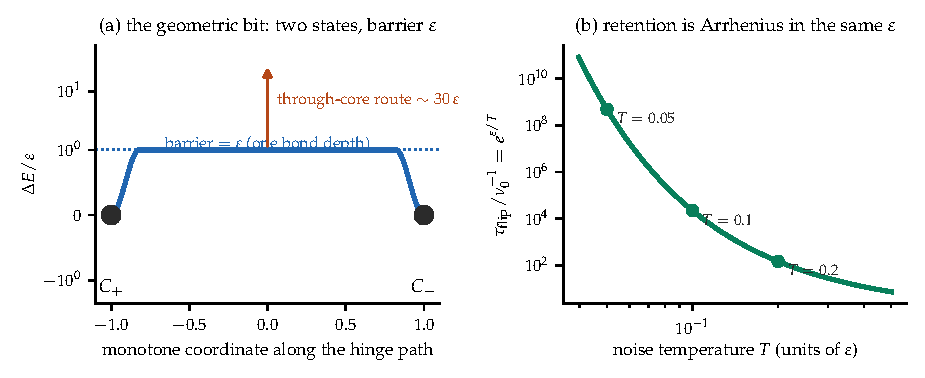
\includegraphics[width=\textwidth]{register.pdf}
\caption{The geometric bit. (a) Two mirror states separated by a barrier
of exactly one bond depth along the hinge path; the direct route through
the repulsive core costs about thirty times as much. The matching lower
bound is an exact plane-crossing argument plus an outward-rounded interval
certificate with zero uncertified boxes. (b) The
same $\varepsilon$ enters the Kramers/Arrhenius retention estimate under
its stated weak-noise and damping assumptions.}
\label{fig:register}
\end{figure}

Both purchases so far were quoted in the same unit, $\varepsilon$, and
neither section said what fixes it or what it costs to keep paying.
That is a thermodynamic question --- a barrier is only a barrier
relative to a temperature --- and it is the subject of the next
section.

% =====================================================================
\section{Thermodynamics: noninvertibility, retention, and timescale}
\label{sec:thermo}

Thermodynamics enters this architecture at three places. The distinctions
below are deliberately narrower than the slogan that actualization ``uses
energy and cannot be undone.'' They separate a many-to-one record map, a
metastable memory, and a complete thermodynamic entropy balance; only the
first two are supplied here.

\paragraph{Singularity, readout loss, and full noninvertibility are
different claims.} Postulate~\ref{post:A} declares that one outcome enters
history [IMPOSED]. Identifying the model's manifestation/genesis rule with
that actualization block is a proposed physical identification
[CONJECTURE]. For a fixed context $M$, write its discrete readout as
\begin{equation}
  \mathcal R_M:X_M\longrightarrow O_M,
  \qquad x\longmapsto o.
  \label{eq:actualizationmap}
\end{equation}
The genesis readout is many-to-one: distinct continuous flux magnitudes can
yield the same discrete record [MEASURED, engine-scoped]. The continuous
flux itself remains stored, so this does \emph{not} prove that genesis
erases the complete microstate. Full-map noninjectivity is established
separately by an evaporation witness: two distinct admissible engine states
evolve to one identical persistent state [THEOREM, current-engine scope].
The honest statement is therefore that the candidate readout is lossy and
the current complete update is noninjective, not that every manifestation
event erases all information.

This separation also fixes the word \emph{unchoose}. The discrete record
does not reconstruct the continuous preimage or turn a counterfactual into
the event that occurred. Reversing an enlarged microscopic state, if one
exists, is a different operation from reading the inverse of
\eqref{eq:actualizationmap}.

\paragraph{What ``energy-paid'' means here.} The accepted genesis map has a
positive drain and is non-symplectic under the model's standard $(J,W)$
canonical pairing. A branchwise symplectic, energy-conserving lift exists
only after record-bearing bath variables and feedback are added
[THEOREM, model-scoped]. At positive drain at least three canonical bath
pairs are required for that selected pairing; after one event the bath is
loaded and a fixed zero-bath section cannot be reused unchanged. Repeated
operation therefore requires reset, replacement, export, or active
feedback. One declared implementation test also removes about $37\%$ of
the field norm [MEASURED, implementation-scoped]. Neither number is a
universal measurement-energy quantum or a complete heat/entropy balance.

\paragraph{The imposed bath is an operational thermostat.} The stochastic
element in the measurements of Section~\ref{sec:born} is an
Ornstein--Uhlenbeck thermostat on the field velocity, and it is not
decorative: it equipartitions, delivering $\langle|v|^2\rangle = 3T$ per
site to within a few per cent, with an autocorrelation decaying at the
declared rate. It is, however, \emph{imposed}: the underlying dynamics is
deterministic and supplies no ensemble of its own. Every probabilistic
statement in this paper inherits that qualification.

\paragraph{Retention is Arrhenius; reset cost is a separate question.}
Proposition~\ref{prop:registerbarrier} put the barrier at one bond depth,
and Section~\ref{sec:register} gives $\tau_{\rm flip}\sim\nu_0^{-1}
e^{\varepsilon/T}$. A register is therefore not free: holding one bit for
$N$ clock cycles requires $\varepsilon/T \gtrsim \ln(N\,\nu_0 T_{\rm
clock})$, so the required barrier grows logarithmically with the desired
retention depth --- equivalently, achievable retention grows exponentially
with $\varepsilon/T$. The model's statics supply the barrier
value; the exponential form is imported Kramers rate theory under the
imposed bath, and inherits its premises. This is a reliability bound, not
an energy ledger for one selection. If a later reset logically erases one
unbiased bit in an equilibrium bath, Landauer's bound supplies
$W_{\rm reset}\ge k_BT\ln2$~\cite{landauer}; no such reset cycle or heat
flow is constructed here. Energy dissipated to an untracked environment
cannot be recovered by simply reversing the retained record, but the amount
dissipated per actualization remains \textbf{open}. Figure~\ref{fig:epsilon}
states the resulting, narrower economy.

\begin{figure}[t]
\centering
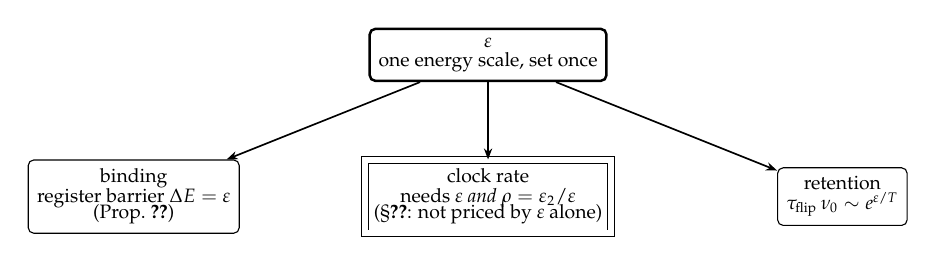
\begin{tikzpicture}
\node[thm] (eps) at (0,0) {$\varepsilon$\\[-1pt]\figsub one energy scale, set once};
\node[sel] (bind) at (-4.5,-1.8) {binding\\[-1pt]\figsub register barrier $\Delta E=\varepsilon$\\[-2pt]\figsub (Prop.~\ref{prop:registerbarrier})};
\node[openb] (clk) at (0,-1.8)   {clock rate\\[-1pt]\figsub needs $\varepsilon$ \emph{and} $\rho=\varepsilon_2/\varepsilon$\\[-2pt]\figsub (\S\ref{sec:toy}: not priced by $\varepsilon$ alone)};
\node[sel] (ret)  at (4.5,-1.8)  {retention\\[-1pt]\figsub $\tau_{\rm flip}\,\nu_0\sim e^{\varepsilon/T}$};
\draw[con] (eps) -- (bind);
\draw[con] (eps) -- (clk);
\draw[con] (eps) -- (ret);
\end{tikzpicture}
\caption{One constant, three bills --- and the bill that did not clear.
The same $\varepsilon$ prices the matter's binding and the memory's
lifetime, at exponents $+1$ and $+1$. It does \emph{not} price the clock
rate: the purchased closure species carries its own depth, so the clock
needs $\rho=\varepsilon_2/\varepsilon$ as well, and $\rho$ moves the
clock while leaving the other two fixed. That is the architecture's own
falsifier --- a measurement moving one of the three without the others
--- and Section~\ref{sec:toy} fires it. The commitment survives for two
of the three bills, and in the leading $A\to0$ quartic normal form
$\Gstar$ itself is independent of $\rho$.}
\label{fig:epsilon}
\end{figure}

\paragraph{And a detector timescale.} In the declared classical threshold
instrument, the quantity controlling the interpolation from amplitude to
action/occupation weighting is not an energy but a ratio of timescales:
the mode frequency against the imposed noise correlation time. Calling
that interpolation ``quantum'' would assume the Born pushforward that the
paper leaves open.

\paragraph{The debt this leaves.} A clock prices duration; a barrier prices
retention; the genesis analysis prices one model-scoped route to writing a
record. None assigns the ensemble law of records, still less the joint law
of responses under incompatible settings. A costly draw from a
setting-independent marble bag is still a draw from the same bag.
Thermodynamics answers how a fact can become stable. It does not answer why
frequencies satisfy the trace rule or why incompatible contexts fail to
glue into one Fine joint distribution. The next section imports the
structure of quantum weights; the physical Born and Bell pushforwards will
remain open after that import.

% =====================================================================
\section{Weights, and where they come from}
\label{sec:operational}

\subsection{The adopted local net and the actual record algebra}

For each finite region $\Lambda\subset\mathbb Z^3$, the actual beables are
bounded functions of classical flux and ternary configurations,
\begin{equation}
 \mathcal A_{\rm act}(\Lambda)=
 \mathcal B_b\!\left((\mathbb R^3\!\times\!\{-1,0,+1\})^\Lambda\right).
 \label{eq:actualalgebra}
\end{equation}
This algebra is commutative. Its finite ternary record subalgebra is the
diagonal algebra
$\mathcal D_\Lambda\cong\mathbb C^{3^{|\Lambda|}}$; it is not the full matrix
algebra $M_{3^{|\Lambda|}}(\mathbb C)$. The potentiality layer is a separately
adopted net $\Lambda\mapsto\mathcal A_{\rm pot}(\Lambda)$ satisfying isotony,
compatible restriction, and commutation for spacelike-disjoint regions. The
first selected witness is
\begin{equation}
 \mathcal A_{\rm pot}^{\rm ref}(\Lambda)=
 \bigotimes_{x\in\Lambda}M_3(\mathbb C).
 \label{eq:qutritnet}
\end{equation}
Its finite-region algebras are Type~I and its quasi-local inductive limit is
UHF. No Type-III conclusion follows automatically: any factor classification
in a GNS representation depends on the chosen state and representation, and
finite random-matrix level statistics cannot decide it.

A preparation map $\Gamma_\Lambda$ from substrate preparation classes to
compatible local states $\omega_\Lambda$ is therefore an adoption with a
named recovery debt. The compatibility condition
$\omega_{\Lambda_2}|_{\mathcal A_{\rm pot}(\Lambda_1)}=
\omega_{\Lambda_1}$ for $\Lambda_1\subseteq\Lambda_2$ is proved by the
selected reference witness and must later be recovered physically. This is an
abstract discrete local net first and a qutrit representation second; the
classical ternary alphabet alone does not derive noncommutativity.

\subsection{States, effects, and convexity}

Two preparations are equivalent if every subsequent experiment gives the
same statistics; the equivalence class is a \emph{state} $\omega$. Two
detector outcomes are equivalent if they have the same probability for
every preparation; the class is an \emph{effect} $e$. The primitive
pairing is
\begin{equation}
e(\omega) \in [0,1],
\end{equation}
read as the potential weight of actualizing $e$ given $\omega$. There is
as yet no Hilbert space, no wavefunction and no Born rule. If $\omega_1$
is prepared with frequency $p$ and $\omega_2$ with frequency $1-p$,
operational consistency forces
$e(p\omega_1 + (1-p)\omega_2) = p\,e(\omega_1) + (1-p)\,e(\omega_2)$, so
the state space is convex and effects are affine. This is the
general-probabilistic level: it contains classical probability,
real-Hilbert quantum theory, and much else.

\subsection{The reconstruction, imported}

What selects complex quantum theory from that class is a separate,
external result. Chiribella, D'Ariano and Perinotti~\cite{cdp} derive
finite-dimensional complex quantum theory from the
operational-probabilistic framework together with six principles:
causality, perfect distinguishability, ideal compression, local
distinguishability, pure conditioning, and purification --- the last
being what separates the quantum member from the classical one. Under
those premises,
\begin{equation}
\mathcal{H}_A \simeq \mathbb{C}^{d_A}.
\label{eq:cdp}
\end{equation}

\begin{scopebox}
\textbf{Status of \eqref{eq:cdp}.} A theorem \emph{external} to this
paper, conditional on its six imported premises. Nothing here derives
those premises from anything more primitive; Appendix~\ref{app:invoice}
itemizes them as an import invoice, which is the honest replacement for
treating ``the Hilbert space'' as a single unpriced assumption.
\end{scopebox}

\subsection{The trace rule from effect additivity}

Once the quantum effect space is in hand, the shape of the weight
functional is fixed by a second declared postulate.

\begin{postulate}[Effect-noncontextual additivity]
\label{post:B}
A weight functional $w:\mathcal{E}(\mathcal{H})\to[0,1]$ with $w(I)=1$
satisfies $w(E+F) = w(E) + w(F)$ whenever $E+F\le I$, for \emph{all}
effect decompositions, including those whose members do not commute.
\end{postulate}

\noindent Postulate~\ref{post:B} is substantive and load-bearing: it is a
noncontextuality of valuation over generalized measurements, and a
contextual valuation escapes what follows without contradiction. From
additivity, $w(qE) = q\,w(E)$ for rational $q$. Monotonicity is derived
rather than assumed --- for effects $E\le F$ the difference $F-E$ is an
effect, so $w(F) = w(E) + w(F-E) \ge w(E)$ --- and squeezing with
rationals $q_n\uparrow\lambda\le r_n\downarrow\lambda$ gives
$w(\lambda E) = \lambda w(E)$ for real $\lambda$. Extending by
differences yields a positive linear functional, and in finite dimension
every such functional is a trace:
\begin{equation}
w(E) = \Tr(\rho_w E).
\label{eq:trace}
\end{equation}
This is Busch's generalized Gleason theorem~\cite{busch}, valid already
in dimension two, where the original Gleason theorem --- which assumes
additivity only over \emph{projective} decompositions --- requires
$\dim\ge3$ and fails. The strengthening from projectors to effects is
exactly the content of Postulate~\ref{post:B}. Throughout this paper,
\eqref{eq:trace} and everything downstream of it is described as
\emph{derived from Postulate~\ref{post:B}}, never as derived
\emph{simpliciter}.

\subsection{Probability is state plus question}

With \eqref{eq:trace} the logical order of Section~\ref{sec:ontology}
becomes formal. For a measurement $M = \{E_i\}$ with $\sum_i E_i = I$,
\begin{equation}
p(i \mid \rho, M) = \Tr(\rho E_i), \qquad \sum_i p_i = \Tr\rho = 1 ,
\end{equation}
so a probability exists only once a question is supplied: the state is
not itself a probability distribution. For a pure state and a sharp
outcome this reduces to the familiar square,
\begin{equation}
p_i = \Tr\big(|\psi\rangle\langle\psi|\,|i\rangle\langle i|\big)
    = |\langle i|\psi\rangle|^2 ,
\label{eq:born}
\end{equation}
which in this architecture is a \emph{theorem about weights} standing at
the end of the chain $|\psi\rangle \to \rho \to (\rho,M) \to p_i$, rather
than an axiom about probability standing at its beginning.

Two structural facts follow immediately and matter later. Global phase
is unphysical, so pure potentiality is a ray and $\psi$ decomposes into a
weight structure and a phase structure, of which squaring retains only
the first. And coherent potentiality is not ignorance over the same
alternatives: for $|\psi\rangle = \alpha|A\rangle+\beta|B\rangle$ the
cross term $2\,\mathrm{Re}\,\alpha^*\beta\langle A|E|B\rangle$ is absent
from the corresponding mixture. That argument excludes one specific
mixture reading; the stronger exclusion of $\psi$-epistemic models is the
Pusey--Barrett--Rudolph theorem~\cite{pbr}, at the price of its
preparation-independence assumption.

\subsection{Dynamics, instruments, and the selector}

Requiring affineness on mixtures, positivity, and positivity under
extension by an untouched ancilla gives complete positivity, so physical
channels are CPTP maps in the instrument tradition of Davies and
Lewis~\cite{davieslewis}. A reversible transformation preserving
pure-state transition probabilities acts on rays and is unitary or
antiunitary (Wigner~\cite{wigner}); for a one-parameter group the
antiunitary branch is excluded because $U(t) = U(t/2)U(t/2)$ and the
square of either is unitary, and the projective obstruction vanishes for
$\mathbb{R}$~\cite{bargmann}, so with strong continuity Stone's
theorem~\cite{stone} gives $U(t) = e^{-itG}$ and, on defining
$H := \hbar G$,
\begin{equation}
i\hbar\,\partial_t|\psi\rangle = H|\psi\rangle, \qquad
i\hbar\,\dot\rho = [H,\rho].
\end{equation}
The existence of a phase generator is structural; the numerical value of
$\hbar$ is empirical and is not derived here. A measurement context is
represented not by an observable but by an \emph{instrument}
$\{\mathcal{I}^M_o\}$ of CP trace-nonincreasing maps summing to a
trace-preserving map, with $E^M_o = (\mathcal{I}^M_o)^*(I)$; an
instrument carries two things at once, the weight of a possible
actualization and the successor potentiality if it occurs.

What the state/effect and instrument architecture does not supply
intrinsically is the selection of one outcome. Writing
$\Sigma_O$ for that block, there are two mathematically distinct
implementations,
\[
\underbrace{K_O(o\mid\rho,M,H)}_{\text{primitive stochastic}}
\qquad\text{or}\qquad
\underbrace{\lambda\sim\mu(\dd\lambda\mid\rho,M,H),\;\;
o = F_O(\rho,M,H,\lambda)}_{\text{context-complete deterministic}},
\]
and in either case the physical content is the requirement that the
resulting frequencies reproduce the weights,
\begin{equation}
(F_O)_*\mu(\{o\}) = \Tr(\rho E^M_o) ,
\label{eq:pushforward}
\end{equation}
called the \emph{Born pushforward} below. V2 supplies the following
\textbf{[IMPOSED reference realization]}. For the complete joint context
$C$, order its outcomes and write $w_o^C=\omega(E_o^C)$. With
$u\in[0,1)$ distributed by Lebesgue measure, set
\begin{equation}
 \Sigma_C(u)=\min\left\{o:
 u<\sum_{j\le o}w_j^C\right\},
 \qquad u_{n+1}=2u_n\bmod1 .
 \label{eq:quantileselector}
\end{equation}
Lebesgue measure is invariant under doubling. The quantile intervals have
exactly the required lengths:
\begin{equation}
 (\Sigma_C)_*\mu_{\rm eq}(o)=\omega(E_o^C).
\end{equation}
The hidden measure is context independent,
$\mu_{\rm eq}(\lambda\mid C)=\mu_{\rm eq}(\lambda)$, while the response map
depends on the complete context and is intentionally nonfactorizable across
Bell wings. Thus the construction proves deterministic contextuality,
measurement independence, and compatibility with the target weights. It is
\emph{not} a Born derivation, because those weights are read to place the
quantile boundaries. The physical programme must recover both the equilibrium
measure and the pushforward from substrate dynamics without target-coded
weights; its first preregistered candidate is the free-flux positive-frequency
density $n=|\phi_+|^2$.

Note that $\Sigma_O$ means the
whole implementation --- the kernel, or the pair $(F_O,\mu)$ --- so that
the measure cannot be hidden inside a deterministic map. Given an
outcome, the successor state is ordinary conditionalization,
$\rho' = \mathcal{I}^M_k(\rho)/p_k$; histories compose by
$P(h) = \Tr[\mathcal{I}^{M_N}_{o_N}\circ\cdots\circ\mathcal{I}^{M_1}_{o_1}(\rho_0)]$,
so the potential histories are plural while the actual history is
singular. Collecting the pieces gives the recursion of
Figure~\ref{fig:ontology},
\begin{equation}
(H_n,\mathcal{C}_n,\mathcal{D}) \xrightarrow{\;\Gamma\;} \rho_n
\longrightarrow \{(e_i,w_i)\}
\xrightarrow{\;K\ \text{or}\ (F,\mu)\;} e_{n+1} \longrightarrow H_{n+1},
\label{eq:recursion}
\end{equation}
in which $\mathcal{C}_n$ is the preparation and control record and
$\mathcal{D}$ the stipulated dynamics. The closure map $\Gamma$ is part
of the scaffold, not a theorem: history alone does not determine a state.

The weight layer is now assembled, at a cost stated line by line. The abstract
local-net axioms and the finite qutrit witness are separate adoptions; the
latter is Type~I, its quasi-local limit is UHF, and any non-Type-I GNS factor
would require an additional state-and-representation argument. But even
granting the adopted net, nothing in this layer says physically
\emph{when} a weight becomes a frequency. That is not a
question about the algebra of weights; it is a question about the
mechanism that reads them out, and about how fast it reads compared with
how fast the thing being read is moving. The next section measures
exactly that ratio.

% =====================================================================
\section{Action/occupation weighting as a detector regime}
\label{sec:born}

\subsection{What a threshold counts}

Consider the simplest possible actualization mechanism: a coherent field
riding on noise, and an event recorded whenever the total crosses a
threshold. Which feature of a mode does such a counter weight?

There are three candidates with different physical meanings. It might
weight by \emph{amplitude squared}, which is what a naive
excess-rate calculation gives at leading order. It might weight by
\emph{energy}, which carries an extra factor of $\Omega^2$. Or it might
weight by \emph{action/occupation} $n = E/\Omega$ --- amplitude squared
times frequency, the classical action variable and the adiabatic
invariant. This endpoint has the same frequency dependence as mode
occupation after the usual relativistic normalization, but that algebraic
resemblance does not make it a quantum probability. The mechanism-level
intuition is narrower: a threshold rate can factor into presentations per
unit time and success per presentation. The deterministic traces below
establish the frequency count and a binary amplitude gate, but do \emph{not}
derive a success law proportional to $A^2$ or their product as occupation.
The noisy interpolation is measured separately. Whether any substrate turns
that classical count into $\operatorname{Tr}(\rho E)$
is the separate Born-pushforward problem.

Figure~\ref{fig:mechanism} draws the counting itself, deliberately
without noise: two modes a threshold cannot tell apart by occupation ---
one tall and slow, one half the height knocking four times as often ---
and two limiting faces of thresholding: presentations counted at a low
level and amplitude gating at a high one.

\begin{figure}[t]
\centering
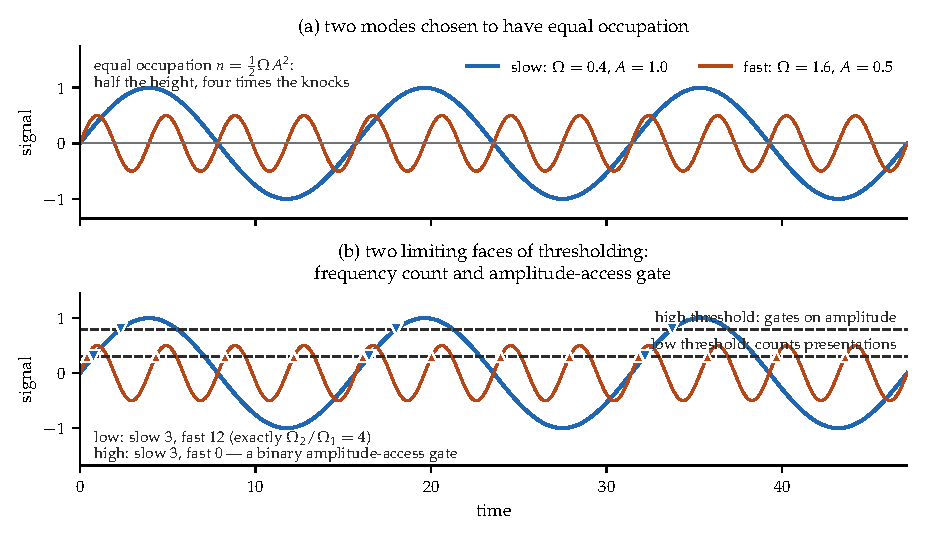
\includegraphics[width=\textwidth]{mechanism.pdf}
\caption{The mechanism, before any measurement. (a) Two modes at equal
occupation $n = \tfrac12\Omega A^2$: the fast one is half the height and
presents four times as often. (b) The same traces against two thresholds,
every crossing computed and marked. At the low threshold both modes
clear, and the counts are exactly in the frequency ratio ($12$ against
$3$): crossings count \emph{presentations}. At the high threshold only
the tall mode reaches, and the fast mode logs zero: \emph{success} gates
on amplitude. A noisy threshold samples between these faces, and the
interpolation between them is measured separately. The hard-threshold trace
does not establish $p_{\rm success}\propto A^2$ and therefore does not by
itself derive occupation weighting. This figure is an illustration on one
declared trace, not a measurement; the measured interpolation between the
two weightings is Figure~\ref{fig:bornregime}.}
\label{fig:mechanism}
\end{figure}

The three classical weighting hypotheses are distinguishable. Preparing two standing modes
at \emph{equal occupation} and regressing the excess crossing rate on
their spatial signatures yields a ratio $R$ whose value is
$\Omega_1/\Omega_2$ under amplitude weighting, $1$ under occupation
weighting, and $\Omega_2/\Omega_1$ under energy weighting. We report the
normalized interpolation coordinate
\begin{equation}
\mathrm{OF} = \frac{R-R_{\rm amp}}{R_{\rm occ}-R_{\rm amp}},
\qquad R_{\rm occ}=1,
\label{eq:occupationfraction}
\end{equation}
the \emph{occupation fraction}. It equals $0$ at the amplitude endpoint
and $1$ at the occupation endpoint. It is a regression coordinate, not an
event probability.

\subsection{The measured interpolation}

Under the author-attested locked protocol --- outcomes, gates, kill
conditions and runner hashes recorded as described in
Appendix~\ref{app:instruments} --- the answer is neither of the three
fixed alternatives. The weighting \emph{interpolates}, and the control
parameter is the product of mode frequency and noise correlation time.
Across five arms spanning $\bar\Omega\tau$ from $0.64$ to $78.36$ the
occupation fraction rises strictly monotonically from $0.049$ to $0.836$
(Table~\ref{tab:born}, Figure~\ref{fig:bornregime}), with a descriptive
crossover near $\bar\Omega\tau \approx 17$.

\begin{table}[t]
\centering
\small
\begin{tabular}{lrcc}
\toprule
Instrument & $\bar\Omega\tau$ & occupation fraction & 99\% CI \\
\midrule
saturation scan, arm 1 & 0.64 & 0.0494 & [0.0359, 0.0623] \\
saturation scan, arm 2 & 2.54 & 0.1020 & [0.0898, 0.1144] \\
saturation scan, arm 3 & 10.15 & 0.2735 & [0.2549, 0.2903] \\
saturation scan, arm 4 & 19.59 & 0.4694 & [0.4583, 0.4797] \\
saturation scan, arm 5 & 78.36 & 0.8362 & [0.8130, 0.8612] \\
\midrule
earlier discrimination, slow & $\approx 0.7$ & 0.024 & [0.014, 0.036] \\
earlier discrimination, fast & $\approx 2.7$ & 0.099 & [0.090, 0.109] \\
\midrule
slow-channel test, $f=1$ & 141.7 & 0.9361 & [0.8953, 0.9700] \\
\bottomrule
\end{tabular}
\caption{Occupation fraction~\eqref{eq:occupationfraction} against the
frequency--correlation-time product.
The two instruments are reported separately and are \emph{not} averaged:
the slow points differ by about $0.02$ beyond seed noise, a declared
phase-draw systematic. The last row is a pure slow channel rather than a
sixth arm of the same scan.}
\label{tab:born}
\end{table}

\begin{figure}[t]
\centering
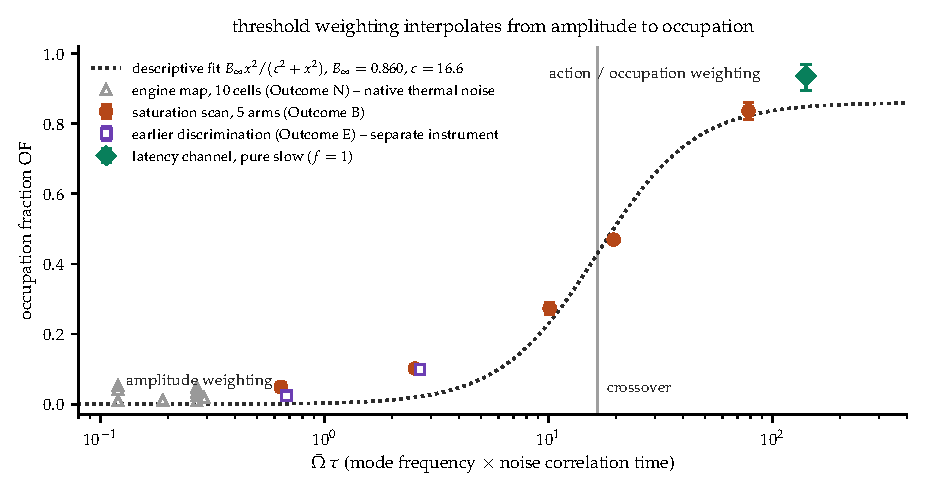
\includegraphics[width=\textwidth]{bornregime.pdf}
\caption{The classical detector measurement. Threshold-crossing statistics
interpolate from amplitude weighting toward action/occupation weighting as
mode frequency exceeds the noise bandwidth. Markers distinguish
instruments deliberately: the two slow-point estimates are never averaged,
the engine cells are a different noise structure spanning only
$\bar\Omega\tau = 0.19$--$0.86$, and the highest point is a pure slow
channel. The dotted curve is descriptive and carries no decision weight.}
\label{fig:bornregime}
\end{figure}

\noindent The reading, at exactly its scope: \emph{within the declared
mechanism class, action/occupation weighting is approached in the
fast-mode/slow-noise regime of a classical threshold statistic}. This is
neither an exact asymptotic law nor a theorem about any substrate; whether
the occupation fraction tends to exactly $1$ or near the descriptive
$0.86$ is open. Identifying the endpoint with quantum outcome probabilities
would require the still-open pushforward~\eqref{eq:pushforward}.

\subsection{The negative, reported at equal prominence}

The same law was then tested where it would matter more: on the model's
own thermal field, with its own propagating noise, under a locked
ten-cell design. \textbf{It did not transfer.} No declared axis reached
the registered structure threshold --- the Spearman correlation of
occupation fraction against the primary axis was $+0.01$, against the secondary
$+0.37$, and against threshold height $-0.20$, all far below the required
$0.7$. The registered outcome is negative.

The post-hoc diagnosis --- and it is flagged as post-hoc, not registered
--- is visible in Figure~\ref{fig:bandmap}: the mean-subtracted noise
correlation time sat pinned between $0.6$ and $1.9$ ticks in every cell
regardless of the thermostat's damping, so the accessible range of
$\bar\Omega\tau$ was only $0.19$--$0.86$, entirely below the crossover.
Within that range the measured values, $0.01$--$0.05$, are quantitatively
consistent with the interpolation law. The structural suggestion is that
thermal noise carried by the field itself can never be slow relative to
that field's own band, because signal and noise are the same medium. We
state that as a suggestion: the record disfavours the route in the
sampled domain and does not prove that it can never succeed.

\begin{figure}[t]
\centering
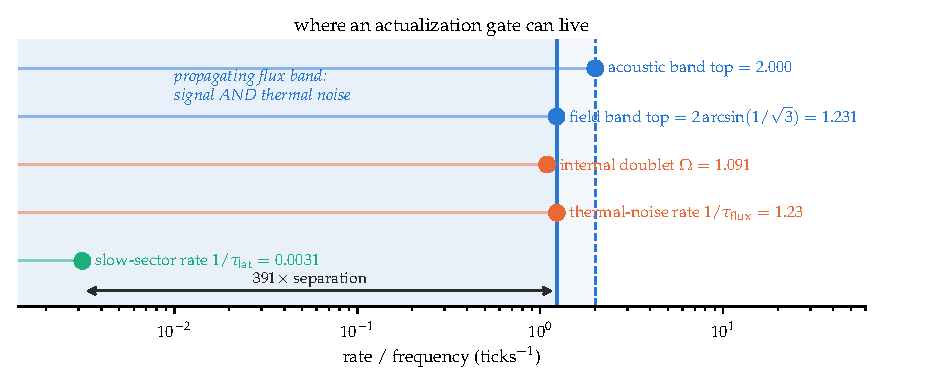
\includegraphics[width=\textwidth]{bandmap.pdf}
\caption{Why the negative may reflect a shared-band limitation in the
sampled design. The propagating band carries both the signal modes and the
thermal noise; in these ten cells the noise rate was not pushed below the
band. A slower channel of different origin --- here the model's slowly
accumulating gravitational-potential sector, three orders of magnitude
slower --- is therefore a candidate location for an actualization gate,
not a demonstrated necessity.}
\label{fig:bandmap}
\end{figure}

\subsection{A slow channel, and the purity requirement}

That diagnosis has a testable consequence: if the gate must be slow and
the field cannot be, the model must be searched for a slow channel of
different origin. It has one --- a slowly accumulating potential sector
sourced by the matter configuration. Measured under its own locked
pre-registration on a self-gravitating configuration with no thermostat
and no manifestation events, its fluctuations have correlation time
$\tau = 317.9$ ticks against the field's $0.81$: a ratio of $391$, and
$\bar\Omega\tau = 141.7$, deep in the regime the interpolation law
identifies.

Feeding a channel at that timescale into the mechanism, with the fast
field noise still present at full strength, gives the result in
Figure~\ref{fig:purity}: the occupation fraction stays pinned between $0.04$
and $0.09$ up to a slow-channel share of $75\%$, and reaches $0.936$ only
when the slow channel is essentially the \emph{sole} stochastic element.

\begin{scopebox}
\phantomsection\label{diag:purity}
\textbf{Measured purity diagnostic [MEASURED --- instrument-scoped].}
\emph{In the additive two-channel model class studied here}, crossing
statistics are dominated by the fastest stochastic component present, so
occupation weighting requires not merely the presence of a slow channel
but its near-exclusivity at the threshold. The evidential base is five
slow-channel shares at $32$ seeds on one instrument. This is an empirical
diagnostic for that class, not a proposition about crossing statistics in
general.
\end{scopebox}

\noindent This is a demanding condition within the declared additive
two-channel mechanism class: a candidate realization in that class would
have to \emph{shield} the actualization comparison from the fast field,
not merely add a slow term to it.  No such necessity has been established
for other detector dynamics.

\begin{figure}[t]
\centering
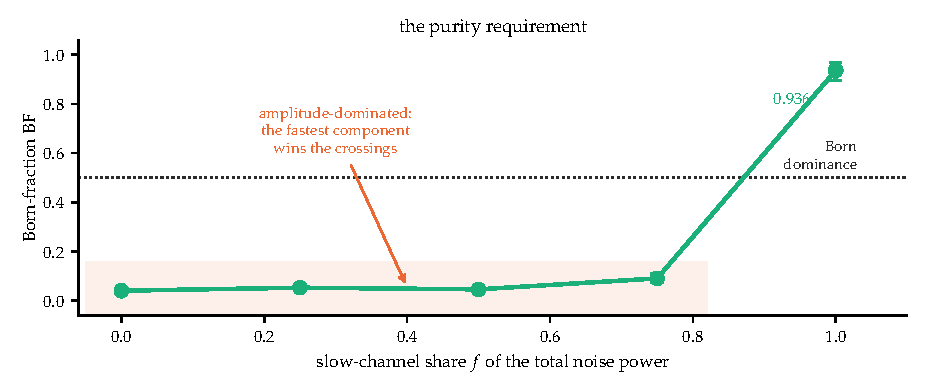
\includegraphics[width=\textwidth]{purity.pdf}
\caption{The purity requirement within the declared additive instrument.
Mixing a slow channel into fast noise does not gradually produce
action/occupation weighting; the classical threshold statistic remains
amplitude-dominated until the slow channel is nearly exclusive.}
\label{fig:purity}
\end{figure}

\subsection{What an irreversible choice does --- and does not --- buy}
\label{sec:irreversiblebell}

The marble example of Section~\ref{sec:ontology} captures two real features
of this ontology. Only the marble actually drawn enters the record, and a
physical draw plus reset can be hysteretic and dissipative. The unrealized
draws remain counterfactual. Neither fact, however, removes Bell's
constraint. Bell does not require all four settings to be performed in one
trial, nor does it require the record-forming dynamics to be reversible. It
asks whether the four possible responses can be represented together on
one setting-independent probability space.

\begin{proposition}[Irreversible choice is Bell-neutral]
\label{prop:irreversiblebell}
Let $x,y\in\{0,1\}$ be the settings, let $\lambda\sim\mu$ be independent of
their choice, and suppose the possible local responses are four functions
$A_x(\lambda),B_y(\lambda)\in\{-1,+1\}$ on that one space. After those
signs are selected, allow an arbitrary \emph{outcome-preserving} physical
write $D_{xy}$ --- including a many-to-one, hysteretic, or
energy-dissipating update of the memory's microstate. Then correlators of
the recorded signs obey $|S|\le2$. Noninvertibility of that write does not
weaken the bound.
\end{proposition}

\begin{proof}
For every $\lambda$ before the record update,
\[
C(\lambda)=A_0(B_0+B_1)+A_1(B_0-B_1)=\pm2,
\]
because one of $B_0+B_1$ and $B_0-B_1$ vanishes and the other is $\pm2$.
Averaging over the single setting-independent $\mu$ gives
$|S|=|\int C\,\dd\mu|\le2$. Any local stochasticity can be included in
$\lambda$. The later map $D_{xy}$ never enters the pointwise identity, so
its invertibility and energetic cost are irrelevant to the inequality. If
a write locally recodes a sign, that recoding can be absorbed into the
corresponding response function. A joint setting-dependent overwrite is
not a counterexample; it abandons the local-response premise.
\end{proof}

The proposition marks the exact boundary of the user's intuition. An
actual choice can be one-way without the unchosen alternatives being
co-actual quantum worlds; that is a coherent ontology of singular records.
But if the bag's marble positions and drawing dynamics define all four
responses on one common ensemble, it remains a classical Bell model. Fine's
theorem makes the joint-distribution boundary exact~\cite{fine}. To reach
$2\sqrt2$, at least one named premise must fail. V2 keeps measurement
independence and ordinary equilibrium probability, but rejects the existence
of four context-free local response variables: $\Sigma_C$ depends on the
complete joint context and does not factorize across the wings. This is an
explicit ontic cost, not an evasion produced by discreteness. The imposed
reference selector reproduces the selected singlet law while keeping each
local marginal independent of the remote setting. Energy-paid record
formation still explains only why an outcome persists; it does not derive the
physical quantum correlation law from substrate dynamics.

\subsection{Three ceilings, and the gap nobody has closed}
\label{sec:tiers}

The architecture's central distinction has so far been qualitative:
potentiality is \emph{structured}, and actuality is singular. Bell
correlations make the first half quantitative, and doing so exposes an
open problem that is the paper's thesis in numerical form.

Three ceilings bound the CHSH quantity, and each corresponds to a
different admissible explanatory structure:

\begin{center}
\small
\begin{tabular}{@{}lll@{}}
\toprule
ceiling & value & structure that could produce it \\
\midrule
local & $2$ & an ensemble of pre-assigned values \\
quantum (Tsirelson~\cite{tsirelson}) & $2\sqrt2 \approx 2.8284$ & a noncommutative weight structure \\
no-signalling (PR~\cite{pr}) & $4$ & a nonsignalling conditional probability assignment \\
\bottomrule
\end{tabular}
\end{center}

Three precisions keep the reading honest.

\emph{The first ceiling is not a bound on actuality.} Every recorded
outcome is actual whatever $S$ turns out to be; actuality is singular per
trial and is not bounded by anything. What $2$ bounds is what
\emph{pre-assigned} values could produce --- the sixteen vertices of the
local polytope are exactly the deterministic assignments in which each
system already carries an answer to both questions it might be asked.
This is why singular actuality and $S = 2\sqrt2$ coexist without strain:
the tension is with pre-assignment, not with actualization.

\emph{The second is a slice, not a shape.} $2\sqrt2$ is the maximal value in the CHSH direction of
the quantum set. That set is nonpolytopal; general membership admits
systematic outer bounds through the NPA semidefinite
hierarchy~\cite{npa}.

\emph{The third is not merely a formal maximum.} Popescu--Rohrlich boxes
attain $4$ while remaining operationally nonsignalling~\cite{pr}.  This
does not establish compatibility with the causal structure of local QFT
or AQFT.  The outer ceiling is what nonsignalling probabilistic
consistency alone permits.

That last point is the substance. \textbf{No-signalling and probabilistic
consistency alone do not explain why nature stops at $2\sqrt2$.} The
no-signalling set extends to $4$; the quantum ceiling uses $70.7\%$ of that
range and leaves the rest excluded. Several principles have been proposed that recover
Tsirelson's bound or approach it --- information
causality~\cite{infocausality}, macroscopic locality~\cite{macroloc},
local orthogonality~\cite{localorth}, and limits on communication
complexity~\cite{vandam} --- and none is established as \emph{the}
derivation.

Figure~\ref{fig:tiers} computes all three ceilings, and adds what the
number buys. Device-independent certification turns $S$ into a resource:
at $S=2$ the outcomes could have been written down in advance and the
certified min-entropy is exactly zero, while at $2\sqrt2$ it is exactly
one bit. Whatever fixes the ceiling therefore fixes how much
unpredictability the world makes available --- a physical quantity, not a
bookkeeping one.

\begin{figure}[t]
\centering
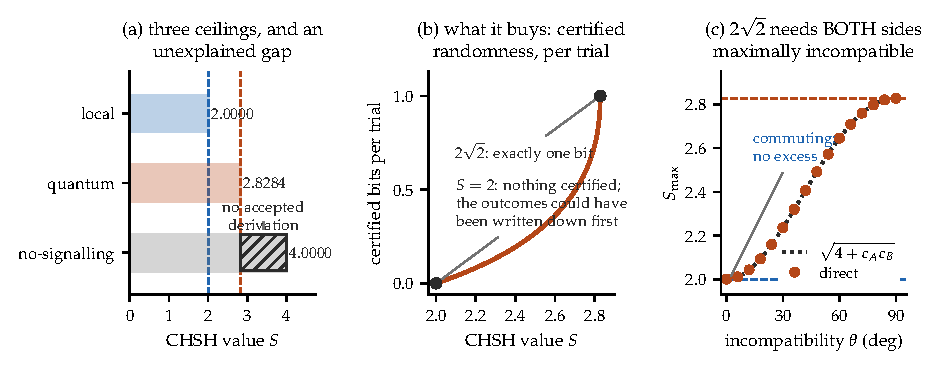
\includegraphics[width=\textwidth]{tiers.pdf}
\caption{The three ceilings, computed. (a) Local correlations stop at
$2$, quantum at $2\sqrt2$, and no-signalling at $4$; the hatched band is
the $29.3\%$ of the no-signalling range above the quantum ceiling. (b) What
the number buys: the device-independent min-entropy runs
from exactly zero certified bits at $S=2$ --- where the outcomes could
have been written down in advance --- to exactly one bit at $2\sqrt2$.
(c) The operator-norm ceiling for dichotomic observables obeys
$S_{\max}^2 = 4 + \lVert[A_0,A_1]\rVert\,\lVert[B_0,B_1]\rVert$:
each commutator norm is capped at $2$, so a product of $4$ requires both
at maximum. There is no partial-credit route to $2\sqrt2$. The dotted
curve is the identity and the markers are the directly computed operator
norm; they agree to $2\times10^{-15}$.}
\label{fig:tiers}
\end{figure}

Within the adopted commuting-wing operator model, the usual CHSH square
identity gives $\|\mathcal B\|\le2\sqrt2$. Consequently a PR-box value of
$4$ is rejected inside this reference architecture, even though it satisfies
no-signalling. The selected singlet state and observables saturating the
quantum ceiling remain imported reference data, not substrate outputs.

The architecture therefore acquires a quantitative form and an open
problem in the same stroke. The potential is not ``whatever is not
forbidden'': it is a specific, tightly constrained subset of the
consistent, and the constraint has no accepted explanation. Whatever
fixes the weight structure of Section~\ref{sec:operational} is the same
thing that fixes this ceiling, and neither the reconstruction programme
nor anything in this paper supplies it. The gap between $2\sqrt2$ and $4$
is the width of that ignorance, measured.

\subsection{What the angles do, and which part needs a record}
\label{sec:angles}

One further separation is worth making explicit, because two claims are
commonly run together and only one of them is true.

\begin{figure}[p]
\centering
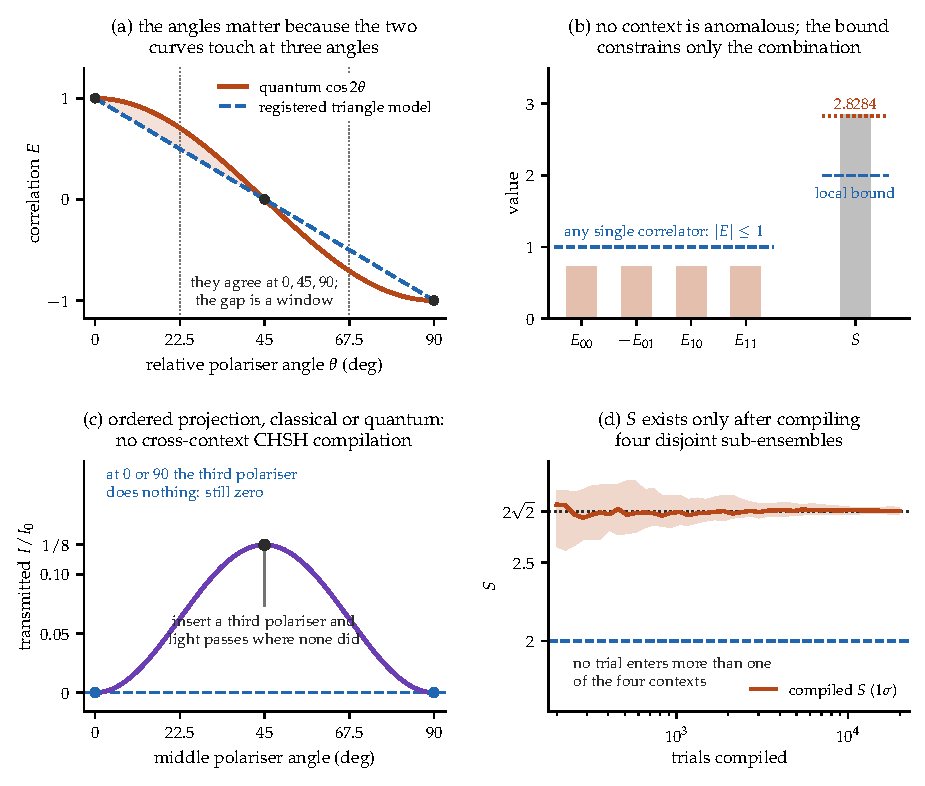
\includegraphics[width=\textwidth]{bellangles.pdf}
\caption{The angles, and the boundary. (a) For polarisation-entangled
light the quantum correlation $\cos2\theta$ and the registered
deterministic sign-threshold triangle model \emph{touch} at $0^\circ$,
$45^\circ$ and $90^\circ$; analytically the largest positive separation from
that model is $0.210514$ at $19.7701^\circ$. This line is not a universal
pointwise locality bound; locality constrains the cross-context CHSH
combination. (b) At the CHSH settings each of
the four contexts contributes exactly $1/\sqrt2$, well inside the
$|E|\leq1$ available to any correlator: no context is individually
anomalous, and the local bound constrains only the total. (c) Two crossed
polarisers transmit nothing; inserting a third at $45^\circ$ transmits
$I_0/8$. Classical Jones/Maxwell optics and quantum single-photon optics
both reproduce this order-dependent projection. It needs an output readout,
but no cross-context CHSH compilation. (d) $S$
by contrast is a compiled statistic: the four sub-ensembles are verified
disjoint and exhaustive, no trial enters more than one, and the number
exists only after all four are combined.}
\label{fig:bellangles}
\end{figure}

\emph{The CHSH number is a construction.} Its four correlators are
measured on four disjoint sub-ensembles; no trial contributes to more than
one; and no individual context is anomalous --- each sits at $1/\sqrt2$,
comfortably inside the unit bound available to any correlator whatever.
$S$ is assembled, and it does not exist without something that assembles
it. This is Fine's gluing statement in operational dress~\cite{fine}, and it is
correct.

\emph{Order dependence is not CHSH compilation.} Two crossed polarisers pass
nothing; insert a third at $45^\circ$ and $I_0/8$ passes. That sequential
projection is reproduced by classical Jones/Maxwell optics as well as by
quantum optics, so it is not by itself evidence for uniquely quantum
observable noncommutativity. It does show that an ordered physical process
need not wait for four-context statistical compilation. Quantum
noncommutativity has independent consequences.  For the canonical
harmonic oscillator, $[x,p]=i\hbar$ together with
$H=p^2/(2m)+m\omega^2x^2/2$ yields $E_0=\hbar\omega/2$; noncommuting
dichotomic observables enter the CHSH operator-norm bound below.

The distinction matters for the architecture. The commutator is the
\emph{input} to $S_{\max}^2 = 4 +
\lVert[A_0,A_1]\rVert\lVert[B_0,B_1]\rVert$ --- an identity for the
operator norm, and a \emph{bound} on any state's observed $\langle
S\rangle$ --- and that observed value is the \emph{readout}
(Figure~\ref{fig:bellangles}). Records are required to estimate the
correlators and compile the observed $S$, while the abstract operator
algebra fixes the quantum ceiling before that compilation. This separates
the algebraic premise from its statistical readout; the three-polariser
example illustrates order dependence but does not decide the ontology of
the quantum commutator.

\begin{scopebox}
\textbf{Scope of Section~\ref{sec:born}.} All ensembles are imposed; the
mechanism-level measurements run on a standalone instrument rather than
the full model; the coupling in the last experiment is a declared
additive model class. The slow-channel measurement's profile contains no
random-number consumer, so its run is fully deterministic and its
seed-independence is vacuous --- configuration-varied robustness is a
registered refinement, not a completed check. None of this establishes a
Born law for any substrate. The tier structure of
Section~\ref{sec:tiers} is a restatement of established bounds, not a new
result; its contribution is to locate the paper's open question inside
them.
\end{scopebox}

Everything established to this point is a \emph{one-frame} statement: a
regime condition read on one instrument, a ceiling fixed by one
algebra, a clock ticking where it was built. Relativity is the demand
that two frames agree, and it is the first obligation in this paper
that cannot be discharged by any single apparatus, however good.

% =====================================================================
\section{Relativity}
\label{sec:relativity}

The architecture divides cleanly under relativity, and the division is
the paper's organizing claim about what merges and what does not.

\subsection{The weight layer relativizes; this is standard physics}

Covariant potentiality is the assignment of local algebras to spacetime
regions with Einstein causality,
$[\mathcal{A}(O_A),\mathcal{A}(O_B)] = 0$ for spacelike-separated
regions~\cite{haagkastler,haag}, with probabilities given by the
state--effect pairing $p_\omega(E) = \omega(E)$ --- the
representation-independent replacement for the trace. Continuum AQFT local
algebras may be non-Type-I and admit no intrinsic density matrix; this is an
external comparator, not a classification of the finite qutrit net in
\eqref{eq:qutritnet}.
Covariant evolution of the potential layer is the Tomonaga--Schwinger
equation~\cite{tomonaga}, conditional on integrability. And for
causally disjoint local instruments the joint statistics are independent
of composition order,
\begin{equation}
p_\omega^{A\prec B}(a,b|x,y) = p_\omega^{B\prec A}(a,b|x,y),
\label{eq:R3}
\end{equation}
provided the instruments satisfy a causal local measurement
scheme~\cite{fewsterverch}. Equation~\eqref{eq:R3}, not trace
preservation alone, is the operational statement that the order of
spacelike instruments is gauge at the level of ensembles. V2 packages a
Bell trial as one \emph{ActualizationBatch}: the wing instruments remain
localized, commuting, and order independent, while the preferred-tick
selector consumes the complete joint context and produces the joint record.
For every admissible batch its local marginals must be independent of the
remote setting.

\paragraph{Order-independence is not selector covariance.}

It is tempting, and wrong, to conclude that a covariant weight layer
delivers a covariant selector. Let $\mu_f$ be the measure over complete
realized histories induced by a selector law under foliation $f$, and let
$\tau_{f\to g}$ exchange only the birth order of spacelike-incomparable
events. The two genuinely distinct further conditions are
\begin{equation}
\mu_g = (\tau_{f\to g})_*\mu_f
\qquad\text{and}\qquad
(\pi_{\mathcal{E}})_*\mu_{f_0} = P^{\rm cov}_{\mathcal{E}}
\ \ \text{for every experiment } \mathcal{E},
\label{eq:R4}
\end{equation}
the first requiring genuine equivariance and the second requiring only
that a physically fixed preferred foliation $f_0$ be operationally
hidden. \textbf{Neither follows from \eqref{eq:R3}}, which contains no
selector law and no history measure. Keeping these apart is, in our view,
the single most common conflation in discussions of relativistic
collapse.

\subsection{Four representative responses, each priced}

\label{sec:responses}
The available responses are families rather than an exhaustive
classification, and they are not mutually exclusive.

\emph{No selector.} Deny Postulate~\ref{post:A}: unitary theory only, and
the covariance problem disappears because there is nothing to make
covariant~\cite{everett}. The price is symmetric and real --- the Born
weights must then be derived without a selector, whether by
decision-theoretic argument~\cite{deutsch,wallace}, contested at length
by Kent~\cite{kent}, or envariance~\cite{zurek}.

\emph{Hypersurface-relative conditionalization.} Take the state update to
be conditionalization and let it be hypersurface-relative, as
in~\cite{aharonovalbert,myrvold}. This is update semantics; it does not
by itself say which event becomes actual or with what measure.

\emph{Covariant stochastic flashes.} Take the actualization events
themselves as the primitive ontology~\cite{bell}, for which
relativistic models exist for fixed particle number, originally without
interaction~\cite{tumulka06} and subsequently with
interaction~\cite{tumulka20}. Indistinguishable particles, variable
number, and full interacting field theory remain open.

\emph{A real preferred foliation.} Let the selector act on a real but
hidden foliation. This makes a total actualization order well defined,
and it is where the discrete model of this paper sits, since a global
tick order is one of its axioms. The empirically required price is
operational hiding --- the second condition in \eqref{eq:R4} --- plus
ordinary Lorentz recovery in every observable sector. Strong history
equivariance, the first condition, is a separate ontological demand and
need not be accepted by a genuinely preferred-foliation theory.
Section~\ref{sec:proofs} conditionally reduces the hiding obligation;
Lorentz recovery remains only partial.

\subsection{Reducing the hiding debt, and locating the Lorentz debt}
\label{sec:proofs}

The two empirical checks owed by a preferred-foliation ontology are not
symmetric. Strong history equivariance is tracked separately.

\begin{proposition}[Operational hiding is not an independent obligation]
\label{prop:hiding}
Let a selector on a fixed foliation $f_0$ generate a measure $\mu_{f_0}$
over complete histories. If \textup{(i)} the marginal of $\mu_{f_0}$ on
recorded data equals the quantum composed-history weight
$P(h) = \Tr[\mathcal{I}^{M_N}_{o_N}\circ\cdots\circ
\mathcal{I}^{M_1}_{o_1}(\rho_0)]$ for every experiment, and \textup{(ii)}
those weights satisfy \eqref{eq:R3}, then
$(\pi_{\mathcal{E}})_*\mu_{f_0} = P^{\rm cov}_{\mathcal{E}}$ for every
operational experiment: the foliation is operationally hidden.
\end{proposition}

\begin{proof}
By (i) the recorded distribution is $P(h)$. By (ii) $P(h)$ is unchanged
when spacelike-separated instruments are exchanged in composition order,
and two admissible foliations of one experiment differ exactly by such
exchanges; so $P(h)$ is foliation-independent and equals
$P^{\rm cov}_{\mathcal{E}}$.
\end{proof}

The proof is nearly immediate once the hypotheses are stated, and its
value is relocation rather than resolution: hiding a preferred foliation
requires nothing beyond reproducing quantum statistics. It is one-way ---
foliation-independent statistics need not be quantum --- and it does not
deliver the stronger equivariance of \eqref{eq:R4}'s first equation,
which concerns unobservable history detail and is presumably false for a
genuinely preferred foliation. Strong equivariance is not required for
empirical adequacy; operational hiding is.

The corollary is more informative than the proposition.

\begin{proposition}[The barrier is not relativistic]
\label{prop:barrier}
If a substrate's four CHSH observables are functions on one sample space
under a single setting-independent measure, their pushforward is a joint
distribution and Fine's theorem gives $|S|\le2$. Hypothesis \textup{(i)}
of Proposition~\ref{prop:hiding} then fails on Bell experiments, and with
it operational hiding. By Proposition~\ref{prop:irreversiblebell}, making
the outcome update noninvertible or energy-dissipating does not alter this
conclusion.
\end{proposition}

\noindent Exhaustive enumeration gives $\max|S| = 2$ over all sixteen
deterministic joint assignments against the attained quantum
$2\sqrt2 = 2.828427$, while the order-independence half of
Proposition~\ref{prop:hiding} checks numerically to $2.2\times10^{-16}$
over random states and settings. So: \emph{if a substrate reproduced
quantum statistics, its preferred foliation would automatically be
hidden.} The v2 reference selector evades the corollary's common-response
premise by using a complete-context, nonfactorizable map while retaining a
setting-independent equilibrium measure. That is a consistency witness only.
The physical difficulty is recovering the same statistics from substrate
dynamics without target-coded weights, and that obstacle is Bell-theoretic
rather than relativistic --- it would be present in a non-relativistic world.
Figure~\ref{fig:reductions} draws the two propositions as one diagram:
what buys hiding, and where the one blocked path actually is.

\begin{figure}[t]
\centering
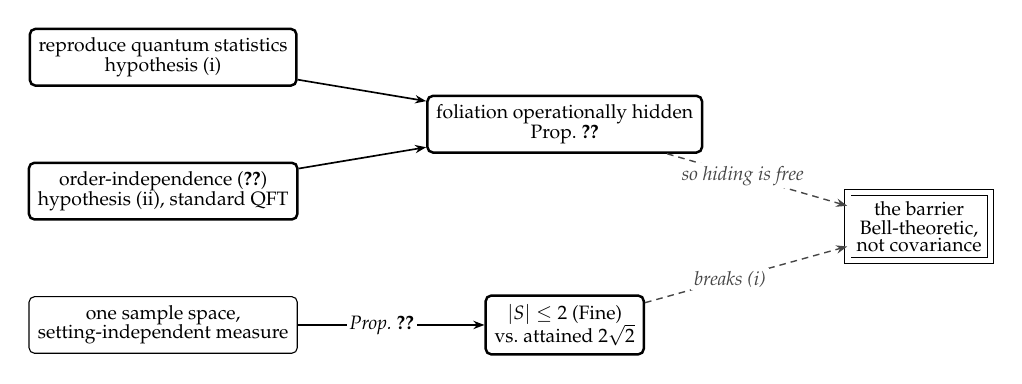
\begin{tikzpicture}
\node[thm] (stats) at (0,0.85)    {reproduce quantum statistics\\[-1pt]\figsub hypothesis (i)};
\node[thm] (ord)   at (0,-0.85)   {order-independence \eqref{eq:R3}\\[-1pt]\figsub hypothesis (ii), standard QFT};
\node[thm] (hid)   at (5.1,0)     {foliation operationally hidden\\[-1pt]\figsub Prop.~\ref{prop:hiding}};
\node[sel] (samp)  at (0,-2.55)   {one sample space,\\[-1pt]\figsub setting-independent measure};
\node[thm] (fine)  at (5.1,-2.55) {$|S|\le2$ (Fine)\\[-1pt]\figsub vs.\ attained $2\sqrt2$};
\node[openb] (bar) at (9.6,-1.3)  {the barrier\\[-1pt]\figsub Bell-theoretic,\\[-2pt]\figsub not covariance};
\draw[con] (stats) -- (hid);
\draw[con] (ord)   -- (hid);
\draw[con] (samp)  -- node[lbl,pos=0.45] {Prop.~\ref{prop:barrier}} (fine);
\draw[wk]  (fine)  -- node[lbl,pos=0.42] {breaks (i)} (bar);
\draw[wk]  (hid)   -- node[lbl,pos=0.42] {so hiding is free} (bar);
\end{tikzpicture}
\caption{The two reductions in one picture. Hiding a preferred foliation
follows from reproducing quantum statistics together with standard
order-independence --- it is not an independent obligation. What blocks a
locally factorized substrate is the lower path: a single setting-independent
joint assignment caps CHSH at $2$ against the attained $2\sqrt2$, which
breaks hypothesis~(i) directly. V2 preserves measurement independence but
rejects that joint assignment through a globally contextual selector. The
open obligation (double-ruled) is physical recovery of that response law,
which would exist even in a non-relativistic world.}
\label{fig:reductions}
\end{figure}

The second debt is real, and its free sector can be paid exactly. The
model's Laplacian is the eighteen-point operator
$\tfrac13\sum_{\rm face} + \tfrac16\sum_{\rm edge} - 4$, whose symbol
expands (in exact arithmetic) to
\begin{equation}
L(\mathbf{k}) = -k^2 + \tfrac1{12}\big(k^2\big)^2
- \tfrac1{360}\Big(\textstyle\sum_i k_i^6
+ 5\sum_{i\neq j}k_i^4k_j^2\Big) + O(k^8).
\label{eq:symbol}
\end{equation}
The fourth-order term is a perfect function of $k^2$: \textbf{the stencil
is isotropic through fourth order}, and structurally so --- the naive
seven-point operator has fourth-order coefficient
$\tfrac1{12}\sum_i k_i^4$, which is not, and the twelve edge terms are
exactly what cancels it. The leading anisotropy is therefore pushed to
sixth order, giving a fractional direction-dependent phase velocity
\begin{equation}
\left|\frac{\Delta v}{v}\right|_{\langle100\rangle-\langle111\rangle}
= \frac{(ka)^4}{3240} + O\big((ka)^6\big).
\label{eq:aniso}
\end{equation}
If one inserts the calibration $a=\ell_P$ and treats a photon-scale
momentum as the free scalar's $k$, the highest observed gamma-ray scale
gives the formal value $1.4\times10^{-56}$, far below optical-cavity
isotropy bounds near $10^{-18}$.  This is a conditional parametric
momentum-scale insertion, not a photon prediction: no photon carrier or
cosmic-ray bound-state pole is constructed here.  It serves only to
calibrate the tree-level stencil term.

\paragraph{Radiative stability: the tree-level result and the unpaid loop problem.}
\label{sec:radiative}

Equation~\eqref{eq:aniso} is a tree-level statement, and a small
tree-level number is not by itself evidence of Lorentz recovery. The
standard objection is that a Planck-suppressed dimension-six violation,
inserted in a loop whose integral is dominated by the cutoff, generates a
\emph{dimension-four} violation with coefficient of order $\alpha/\pi$,
requiring tuning of order $10^{-20}$ against observation~\cite{collins}.
The spatial stencil does contain one useful exact result, but it does not
close that objection.

For a general cubic-symmetric
eighteen-point operator with face weight $w_f$ and edge weight $w_e$, the
continuum limit requires $w_f + 4w_e = 1$ and isotropy of the $k^4$ term
requires $w_f = 2w_e$; together these have the unique solution
$w_f = \tfrac13$, $w_e = \tfrac16$ --- the production weights. There is
no free parameter in this \emph{tree-level spatial improvement} to be
tuned. Averaging a scalar spatial rank-two form $c_{ij}k_ik_j$ over the
cubic group leaves $c_{ij}\propto\delta_{ij}$.

That statement is much narrower than dimension-four Lorentz protection.
Cubic symmetry does not relate temporal and spatial kinetic coefficients,
electric and magnetic terms, or independently renormalized sectors, and it
permits native-vector gradients such as
$\sum_i(\partial_iJ_i)^2$. For a single propagating cone with
$\omega^2=c_0^2(1+\epsilon)k^2$, the
rescaling $t\to t/\sqrt{1+\epsilon}$ removes $\epsilon$ completely: that
sector's speed \emph{is} the definition of the speed, and there is
nothing to compare it against. With two sectors the same rescaling leaves
$(1+\epsilon_2)/(1+\epsilon_1)$, so only the difference survives. This is
one unit redundancy, not a symmetry protection mechanism.

\begin{proposition}[Tree-level scalar spatial reduction]
\label{prop:radiative}
Within the declared scalar eighteen-point spatial stencil, the production
weights are the unique face/edge weights giving the normalized continuum
term and isotropy through $O(k^4)$. A global time rescaling can normalize
one cone. Neither fact constrains all symmetry-allowed dimension-four
operators or the relative cones of interacting sectors.
\end{proposition}

\noindent In particular, saying that a dimension-six operator merely
renormalizes itself misses the dangerous channel: loops can feed a
symmetry-allowed dimension-four operator. The project's frozen
QED-like branch does not find its bare common cone to be a one-loop fixed
point without a dimension-four counterterm. That off-shell coefficient is
scheme-dependent and is not yet an on-shell observable, so it is evidence
against automatic protection rather than a completed phenomenological
calculation.

\begin{scopebox}
\textbf{Status: open --- hard.} The exact result is a tree-level spatial
symbol identity. Radiative closure requires an inventory of every
symmetry-allowed low-dimension operator for one frozen interacting action,
followed by on-shell matching of the full two-point mixing matrix. After
one time normalization is removed, every remaining relative-cone
eigenvalue must be tested. Any required counterterm is imposed, not
emergent. Physical Lorentz invariance is not established here.
\end{scopebox}

\subsection{Where the remaining obligation lives: one body or two}
\label{sec:onetwo}

The preceding results separate two obligations that are often bundled.
Hiding a foliation reduces conditionally to reproducing the quantum
history statistics, whose barrier is Bell-theoretic. A common choice of
units removes one overall cone normalization, but radiative stability does
\emph{not} reduce away: relative temporal/spatial and inter-sector
coefficients remain physical. The useful organizing distinction below is
operational rather than a closure theorem.

Rotations form the little group of a timelike vector: acting on a body's
rest four-velocity $u = (c,\mathbf{0})$, a spatial rotation leaves it
fixed, whereas a boost maps that rest frame to a different one. They are
not independent group factors --- commutators of boosts generate rotations.
There is nevertheless a useful operational contrast. An orientation test
can reorient one apparatus and compare it against itself; a comparison of
standards in distinct rest frames needs clocks and rods that instantiate
those frames. The table is a heuristic for constructed-standard tests, not
an exhaustive partition, and boost-sensitive one-body dispersion tests are
an explicit overlap:

\begin{center}
\small
\begin{tabular}{lll}
\toprule
& \textbf{single-apparatus orientation} & \textbf{cross-frame standards} \\
\midrule
what is compared & apparatus with itself, reoriented & one frame against another \\
typical test & isotropy, sidereal variation & time dilation, cone equality \\
status here & scalar spatial stencil improved at tree level & \textbf{open} \\
\bottomrule
\end{tabular}
\end{center}

The tree-level spatial-symbol result was a statement about the point
group $O_h$ --- a rotation group --- and the residual
\eqref{eq:aniso} is a one-body observable: reorient the apparatus and
look for a sidereal signal. The broader dimension-four and radiative
questions remain open. The cross-frame standard statements are open as
well: whether the matter and field cones agree, whether interacting
vertices preserve a common cone, and whether composite clocks and rods
transform correctly. The single-cone absorption argument of
Section~\ref{sec:radiative} says the same thing from the other side: one
cone can always be scaled to unity, while a \emph{ratio} of two cones is
invariant under every global rescaling and cannot be defined away.

\begin{scopebox}
\phantomsection\label{scope:clockstandards}
\textbf{Operational convention [SCOPE].} Tests that compare rates,
worldlines, or transported standards between frames require physical
standards sufficient to instantiate that comparison. This programme
therefore asks its substrate to construct a clock before claiming an
operational time-dilation test. This is a methodological requirement, not
a theorem that every two-frame observable is mathematically undefined
without two clock parametrizations: geodesic deviation, for example, uses
one reference proper time and a Jacobi field.
\end{scopebox}

\noindent The scope word is load-bearing and an earlier draft omitted it.
Not every boost-\emph{sensitive} quantity needs a constructed clock: the
mass-shell diagnostic of Section~\ref{sec:massivecone} tests a free
dispersion's Lorentz form with no constructed clock, and it is a one-body
calculation. What remains clock-gated
in this programme is the claim that an actual substrate-built clock obeys
the target dilation law.

\noindent This scope distinction reorganizes the recovery contract
rather than discharging it. The one-body dispersion register is computed,
while interacting matter, clocks, and rods remain open. The clock
construction Section~\ref{sec:clock} priced is one concrete missing
standard, not a universal obstruction to defining every relativistic
observable. It is also needed if the stage index is to be read as elapsed
time: Section~\ref{sec:succession} argued that something physical must
carry that index, and Section~\ref{sec:qg} returns to the obligation.

The same restraint applies past special relativity. Operational curvature
requires physical free-fall systems and standards, but geodesic deviation
itself may be parametrized by one reference proper time and a separation
field; it does not prove a universal two-clock gate.

One component of the two-body register can be sharpened immediately. The
model's wave speed $1/\sqrt3$ is not the stability bound: for the
eighteen-point operator the symbol attains $\max|L| = 16/3$ on the face
diagonal, giving $C \le \sqrt3/2$. It is instead exactly the largest
isotropic speed whose round effective cone is \emph{contained} in the octahedral
causal polytope, whose facets $\sum_i \pm x_i = 1$ lie at distance
$1/\sqrt{D}$ from the origin. That is the same $1/\sqrt{D}$ as the
per-axis component of an isotropic unit spread, since
$\mathbb{E}[n_i^2] = 1/D$ for a uniformly random unit vector --- one
isotropic unit distributed over $D$ orthogonal axes, counted two ways.
The characterization is exact, and it relocates the choice rather than
removing it: the containment bound is $1/\sqrt3$ only for six-neighbour
causality, whereas the eighteen-point Laplacian's reach and the model's
stated Moore locality both give $1$. The cone speed is therefore an
interior selection whose adoption carries a commitment about which
neighbourhood defines causal reach.

The neighbourhood is a model definition, but its consequences are exactly
distinguishable. For the stated eighteen-point wave update, a point
perturbation produces first-tick face amplitudes $1/9$, edge amplitudes
$1/18$, and zero corner amplitudes. Six-, eighteen-, and twenty-six-neighbour
support therefore disagree already at $t=1$, and exact dependency can be
tracked symbolically at any amplitude. Machine epsilon is not a support
criterion: it is the relative spacing near unity, not the smallest
representable nonzero number.

What the measurements do show is an \emph{effective} separation of scales.
In the reported point-source run, the amplitude at the M18 support edge
falls by $1.19$ decades per tick --- $2.5\times10^{-7}$ of the peak at
$t=8$, $2.7\times10^{-17}$ at $t=16$, and $2.0\times10^{-26}$ at $t=24$.
That finite-run suppression can make the precursor irrelevant to an
instrument with a declared dynamic range; it does not make strict support
definitional or unobservable in principle.

The strict M18 support is a cuboctahedron, anisotropic by $34.3\%$ between
its face and edge directions. Threshold contours of the measured Green
function are much rounder: $0.71\%$ anisotropy near the effective cone and
$7.2\%$ even fifteen decades down in that run. Their residual anisotropy
decreases empirically as $t^{-1.1}$ to $t^{-1.3}$ depending on probe depth,
consistent with an Airy-front expectation of $t^{-4/3}$. These are measured
effective-field profiles, not the exact causal boundary and not a proof of
a uniform continuum-limit rate.

None of this closes anything. It is a one-body statement --- an
independent cross-check of the free-sector result above by a different
method --- and the obligation that matters is the two-body one.

\subsection{The two-body bill, itemized}
\label{sec:twobodybill}

Six line-items follow. The free massive-mode expansion and the free
multiparticle threshold-cone shift are computed at their stated scope. An
exact symbol decomposition shows how a free cross-sector cone could be
matched, but no working matter sector is built. The static-well
substitution is exploratory and inconclusive under the corrected finite-gap
comparator, while the soliton shape-mode campaign is currently
unreproduced and fails an independent common-cone check. Each item names
what survives and what remains open.

\subsubsection{Free massive modes}
\label{sec:massivecone}

That obligation, however, was bundled too coarsely, and unbundling it
turns part of it into a calculation.

Begin with what will \emph{not} work. The natural test is to take the
clock of Section~\ref{sec:clock}, give it momentum, and compare its period
to $\gamma$. It is vacuous, for the reason recorded when that clock was
bought: a mechanical framework is Galilean invariant and reports zero
dilation whatever the substrate does. Dilation in a field substrate comes
from the binding being mediated at the substrate's own speed --- Lorentz's
electron-theory reasoning, and the light-clock argument in modern dress
--- so the object to interrogate is the \emph{dispersion of a massive
mode}, which needs no clock at all.

For a free mode, a packet around wavenumber $k$ moves at group velocity
$v_g = |\nabla_k\Omega|$. Relativistic mass-shell dispersion implies the
diagnostic
\begin{equation}
\Omega_{\rm shell}(k) = \Omega(k)\sqrt{1 - v_g(k)^2/c^2} = M,
\label{eq:properfreq}
\end{equation}
an identity whenever $\Omega^2 = c^2k^2 + M^2$. This is a mass-shell
diagnostic, not a constructed internal-clock observable: constancy tests
the free dispersion's Lorentz form but does not by itself demonstrate that
a physical clock made from the species dilates. Adding a mass to the
leapfrog gives the exact dispersion
$4\sin^2(\Omega/2) = C^2(-L(k)) + M^2$, and expanding along $[100]$,
$[110]$ and $[111]$ returns \emph{identical} coefficients through $k^4$:
\[
\Omega^2 = \Big(M^2 + \tfrac{M^4}{12}\Big)
+ \Big(\tfrac13 + \tfrac{M^2}{18} + \tfrac{M^4}{90}\Big)k^2
- \Big(\tfrac1{54} + \tfrac{M^2}{1080}\Big)k^4 + \dots
\]
Reading the $k^2$ coefficient as the squared limiting speed,
\begin{equation}
\frac{C_{\rm eff}(M)}{C} = 1 + \frac{M^2}{12} + \frac{19M^4}{1440}
+ O(M^6).
\label{eq:ceff}
\end{equation}

The limiting speed is thus \emph{exactly isotropic} --- the three symmetry
directions agree identically, not approximately --- and \emph{depends on
the rest mass}. The second is a negative result: two species of different
mass do not share a cone exactly. It is the classic species-dependent
maximum-attainable-velocity signature.

Within a species the free dispersion is nearly Lorentzian. Using that
species' own $C_{\rm eff}$, the residual in \eqref{eq:properfreq} is $O(k^4)$ and agrees
with $k^4/(36M^2)$ to within $1.1\%$ over the sampled masses and momenta;
in the physically natural variable $\beta = v_g/C$ this is
\begin{equation}
\frac{\Delta\Omega_{\rm shell}}{\Omega_{\rm shell}}
\simeq \frac{M^2\beta^4}{4}.
\label{eq:dilerr}
\end{equation}
Each mass therefore carries its own very nearly Lorentzian free sector, and the
violation lives in the mismatch \emph{between} masses in this scalar free
sector. If the paper's tick-to-Planck mapping is inserted, electron- and
proton-sized mass parameters give a formal difference
$1.6\times10^{-40}$ and an electron-sized mode at $\beta=0.1$ gives a
residual $1.5\times10^{-50}$. These are parametric evaluations of a
free-mode mass-shell diagnostic, not predictions for physical electrons,
protons, or clocks;
the required matter sectors and interacting matching are not built.

The same expansion reproduces the free-sector anisotropy of
Section~\ref{sec:proofs} independently, giving
$(v_{[100]} - v_{[111]})/C = -k^4/3240$ exactly, which validates the
chain.

One scope limit matters more than the result: this concerns \emph{one
sector with a varying mass}, whereas the far larger problem is that
distinct sectors of the model carry leading speeds differing at order
unity. That problem is the subject of the next subsection, and it turns
out to be the one place in this paper where a stubbornly negative result
inverted.

\subsubsection{A common cone across sectors}
\label{sec:intersector}

One sector can always be given unit speed by choosing the time unit. That
removes one normalization and no more: if two propagating sectors have
slopes $c_A$ and $c_B$, the ratio $c_A/c_B$ survives every common unit
change and is physical preferred-frame data. The discrete model carries
$c^2 = 1/3$ in its production field sector and raw $1$ in a standalone
Wilson matter sector --- an order-unity mismatch, against which the
$10^{-40}$ of the previous subsection is irrelevant. This is the real
obligation.

The first three findings are negative, and sharply so. Writing
$u_i = \cos q_i$, matching a scalar Wilson parameter $r$ to the field
symbol identically,
$c_s^2[3 - \sum u_i^2 + r^2(3-\sum u_i)^2] = \kappa\,(-L_{18})$, gives ten
coefficient equations of which two suffice: the $u_1u_2$ coefficient forces
$\kappa = -3c_s^2r^2$ and the $u_1$ coefficient forces $\kappa = +9c_s^2r^2$,
so $c_s^2r^2 = 0$. \emph{No nontrivial real $(c_s,r)$ gives an exact
all-momentum match.} Second,
the $O_h$-invariant polynomials are generated by $\sum q_i^2$,
$\sum_{i<j}q_i^2q_j^2$ and $q_1^2q_2^2q_3^2$, so the number of isotropy
conditions grows without bound --- cumulatively $0, 1, 3, 6, 10, 16, 23, 32$
through order $q^{16}$. Under naive order-by-order finite-shell tuning,
this is an unbounded sequence of conditions. The counting alone is not a
no-go against a finite all-orders identity: one structure may satisfy
infinitely many Taylor conditions at once, as the seven-square identity
below demonstrates. Third, and
least expected, enriching both structures with a face-diagonal shell yields
six equations in seven Gram monomials, which \emph{solve}; what fails is
realizability. For a real kinetic vector the Gram $A_{st} = a_sa_t$ is an
outer product and must have $A_{11}A_{22}-A_{12}^2 = 0$, whereas the
solution forces $A_{11}A_{22}-A_{12}^2 = \tfrac29\kappa^2$. The required
Gram has rank two; the obstruction is structural, not arithmetic, and being
proportional to $\kappa^2$ it survives every rescaling. Adding the fifth
Clifford structure available to four-component spinors leaves the residual
unchanged; adding a third kinetic shell makes the rank conditions
insoluble.

An economical constructive resolution uses a half-offset carrier basis.
Regrouping and applying
$1-\cos A = 2\sin^2\!\tfrac A2$ and
$1-\cos A\cos B = \sin^2\!\tfrac{A-B}2+\sin^2\!\tfrac{A+B}2$ exhibits the
field symbol as a \emph{sum of squares}, and every argument that appears is
a half-angle.

This factorization does \emph{not} make half-offset sites necessary. For any
integer hop $d$ with graph weight $w$,
\begin{equation}
2w[1-\cos(q\!\cdot\!d)]
=w\sin^2(q\!\cdot\!d)+w[1-\cos(q\!\cdot\!d)]^2 .
\label{eq:integerhop}
\end{equation}
Applying \eqref{eq:integerhop} to the three face-pair hops with $w=1/3$
and six edge-pair hops with $w=1/6$ gives an exact
\emph{eighteen}-square integer-frequency decomposition of $-L_{18}$.
Equivalently, the phase $e^{iq/2}$ in
$e^{iq}-1=2i e^{iq/2}\sin(q/2)$ shows why a half-angle magnitude alone
does not locate endpoints at half sites. Under the termwise Clifford ansatz
below, naively linearizing the eighteen integer-hop squares uses spinor
dimension $512$. The half-angle construction reduces that ansatz's known
exact count to seven, at dimension eight. It is an economy result, not a theorem that the physical lattice must
be refined. If this cheaper basis is physically instantiated, whether it is
read as refined sites or staggered cochains is a separate, open choice.

Under the declared termwise Clifford linearization
$H = \sum_\mu\Gamma^\mu\phi_\mu$, imposing cancellation of every cross term
separately makes the $\Gamma^\mu$ mutually anticommute, and dimension $2^k$
carries $2k+1$ such structures. This is a construction price, not a lower
bound on every matrix factorization: algebraic relations among the
$\phi_\mu$ could permit collective cross-term cancellation. Within this
declared ansatz, the
first decomposition we found was not the shortest, and the difference
matters by a factor of four. Restricting to nearest-neighbour hops on the
half-offset lattice --- degree at most one per variable in $x = q/2$ --- and
writing $s_i = \sin x_i$, $c_i = \cos x_i$, there is an exact and
cubic-covariant decomposition into \emph{seven}:
\begin{equation}
\label{eq:seven}
-L_{18} \;=\; 4\sum_i s_i^2c_j^2c_k^2
\;+\;\tfrac{16}{3}\sum_i s_j^2s_k^2c_i^2
\;+\;4\,s_1^2s_2^2s_3^2 ,
\end{equation}
with $\{i,j,k\}=\{1,2,3\}$. It is checkable by hand: with $A = s_1^2$ etc.,
$S_1 = A+B+C$ and $S_2 = AB+BC+CA$, the three groups contribute
$4[S_1-2S_2+3ABC]$, $\tfrac{16}3[S_2-3ABC]$ and $4ABC$; the triple products
cancel exactly, $12-16+4 = 0$, leaving
$4S_1-\tfrac83S_2 = \tfrac43[3S_1-2S_2] = -L_{18}$. The lone singlet is not
decoration --- it is what kills $ABC$. A search over the same class finds
a non-covariant four-square numerical candidate with fresh-momentum residual
$5.3\times10^{-15}$ and does not find three. No symbolic or interval
existence certificate is supplied for the four. The Hessian rank supplies
the rigorous floor $n\ge3$, while the exact seven below supplies the proven
upper bound, so $3\le n_{\min}\le7$; ``none found at three'' and the
four-square candidate are numerical evidence, not proofs. An exact
cubic-covariant seven-square construction gives the
upper bound $n_{\rm cov}\le7$; mixed-sector covariant constructions with
five or six squares have not been excluded. In the termwise Clifford ansatz,
this seven-square construction uses spinor dimension eight; the numerical
non-covariant four candidate would use four if certified.
\emph{Repository correction.} An older FTD-0798 ledger sentence asserted
a local cubic-covariant three-square decomposition, but supplied neither
the three factors nor a reproducing artifact; a repository-wide search
found no such certificate. That sentence is withdrawn as unsupported. It
does not attain the rigorous floor used here; a recovered exact identity
would have to be published and checked before changing these bounds.
(An earlier draft of this passage reported the minimum as five; its
search drew four hundred starts from a single initialization scale, which
samples one basin many times rather than many basins once. Dispersing the
scale finds the four within tens of starts. The correction is retained
here because the method failure is as instructive as the number.)
Figure~\ref{fig:intersector} draws the mismatch, its cause, one
decomposition, and the price.

If the economical half-angle basis is physically instantiated as hops,
which placement classes appear decides what it costs the primitive ontology.
Three half-offset shells are
available --- face $(\pm\tfrac12,0,0)$, edge $(\pm\tfrac12,\pm\tfrac12,0)$
and body centre $(\pm\tfrac12,\pm\tfrac12,\pm\tfrac12)$ --- and the
restriction now cuts finely: confined to body centres alone the search
reaches five and stalls there over two thousand dispersed starts, while
the best-found numerical four uses the face and edge shells. Thus the
search suggests that leaving the body centres buys one square, but neither
search establishes a minimum. There are two priced readings. On a
refined-site reading, the half offsets are physical sites of a cubic
lattice with spacing $a/2$; that amends the discrete-space postulate and
requires recalibrating $a_{\rm phys}$ and every dimensional prediction
that depends on it. On a staggered-cochain reading, the Bravais spacing
remains $a$ but the theory gains explicit carrier types on cell faces,
edges and bodies. Because the numerical four-square candidate uses face
and edge shells, that reading requires corresponding staggered $1$- and
$2$-cochain content, not merely body-centred sites. Neither reading is
adopted here. Only the cochain reading would leave $a_{\rm phys}$
unchanged. (The stall at four is search evidence of the same kind that
previously mis-reported the minimum, and is offered with exactly that
confidence; the rank bound $n\ge3$ is the only proof in this paragraph.)

The seven-square construction is moreover not a numerical search outcome.
The eight
half-angle triple products $\prod_ig_i(q_i/2)$ with $g_i\in\{\cos,\sin\}$
satisfy $\sum(\prod_ig_i)^2 = \prod_i(\cos^2+\sin^2) = 1$ identically. One
of the eight is the pure cosine $S = \prod_i\cos(q_i/2)$ --- which is
exactly the body-centred-cubic nearest-neighbour structure factor, the eight
neighbours sitting at $(\pm\tfrac12,\pm\tfrac12,\pm\tfrac12)$ --- and the
remaining seven have equal-weight sum
$1-S^2 = (1-S)(1+S)$. Equation~\eqref{eq:seven} is diagonal in that
seven-element half-angle basis, which is why it is spatially
cubic-covariant and why it has seven squares. The factorization aligns it
algebraically with the BCC complement $1-S$, but does not put the usual BCC
Laplacian $8(1-S)$ in the same constant-weight square cone: the extra
factor $1+S$ is load-bearing.

Two consequences deserve stating. Structurally, the optional half-angle
basis aligns algebraically with the body-centred structure factor that also
appears in a Watson-type period identity and an $\mathrm{SU}(3)$ factor.
This is a shared representation pattern, not a derivation that the physical
site lattice must be body-centred. Within the termwise Clifford ansatz, a
mass structure is chosen to anticommute with every kinetic structure, so it costs one
further structure. The numerical four-square candidate would leave one
structure spare and would admit a mass at dimension four \emph{if
certified}; no rigorous low-rank mass price follows yet. The exact
cubic-covariant seven-square construction saturates dimension eight under
that ansatz, so adding a termwise-anticommuting mass to \emph{that
construction} uses dimension sixteen.
A lower-rank mixed-sector cubic-covariant construction could reduce the price and
has not been excluded. (An earlier draft, built on the
mis-reported five, concluded the opposite --- that the minimal carrier was
necessarily massless; that prediction died with the five and is recorded
here so it cannot be cited from memory.)

\begin{scopebox}
\textbf{What this does and does not close.} At the scalar, spatial,
tree-level symbol scope, it shows that exact slope matching is not
algebraically obstructed: there is an explicit decomposition, and its
termwise-Clifford construction price is stated.
It does not deliver a working matter sector. Whether the resulting operator
is an acceptable fermion --- doubling, chirality, and the locality of the
induced interactions --- is untested; the time discretization is a separate
matching problem that can only add conditions; a spinor's worth of
anticommuting structures is not a ternary state, so the carrier must
either \emph{emerge} from the primitive states or be \emph{adopted} as a
new type at a price; and the
order-unity mismatch still stands in the model as it is actually run.
Interacting vertices remain open.
\end{scopebox}

\begin{figure}[p]
\centering
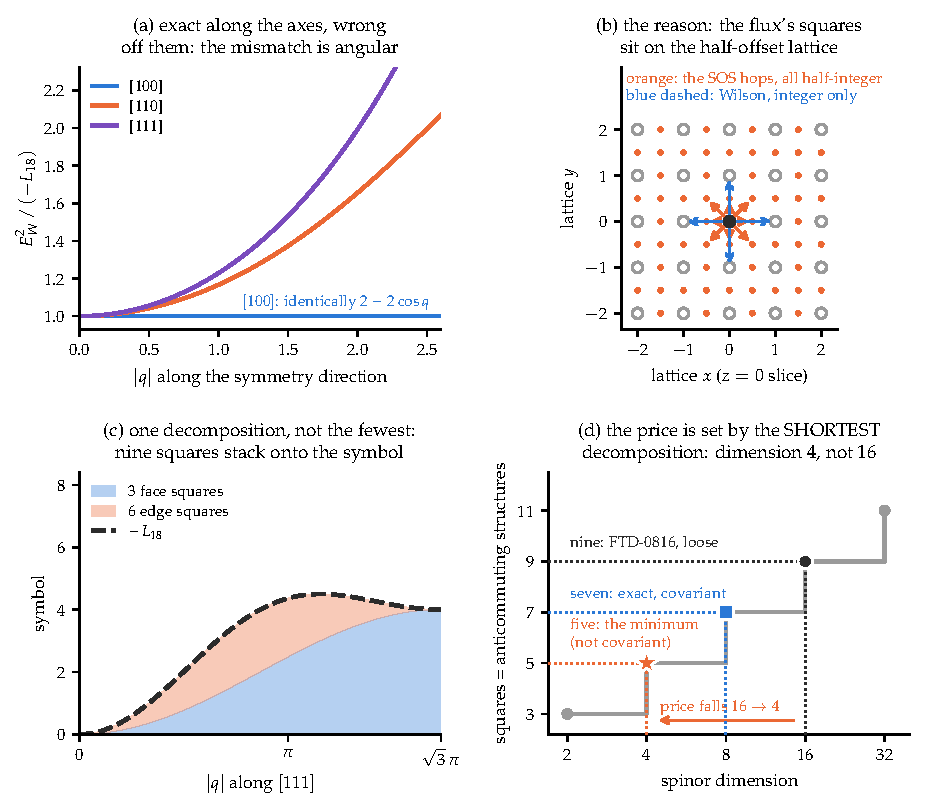
\includegraphics[width=\textwidth]{intersector.pdf}
\caption{Why two sectors miss, and what an exact hit can cost. (a) Normalised to a
common slope, the flux symbol and a Wilson operator agree
\emph{identically} along the cubic axes --- both are $2-2\cos q$ --- and
diverge only off them, reaching $1.65$ along $[110]$ and $1.99$ along
$[111]$ at $|q| = 2$. The mismatch is purely angular, so no rescaling is
even the right shape. (b) Two constructive placement classes in the
$z=0$ slice: the economical half-angle basis uses half-unit face/edge
placements (orange), while an exact but longer integer-frequency
construction uses unit face/edge hops (blue dashed). Half offsets reduce
the known price; they are not forced by existence. (c) One half-angle
identity: three face squares and six edge squares
stack exactly onto $-L_{18}$, with residual $1.8\times10^{-15}$ over
$4000$ random momenta; Equation~\eqref{eq:integerhop} independently gives
an exact eighteen-square integer-hop identity. (d) The known exact and
searched termwise-Clifford prices. Naive Cliffordization sends the integer-hop eighteen to
dimension $512$. An exact spatially cubic-covariant
\emph{seven}-square identity holds,
$-L_{18} = 4\sum_i \sin^2\!x_i\cos^2\!x_j\cos^2\!x_k
+ \tfrac{16}{3}\sum_i \sin^2\!x_j\sin^2\!x_k\cos^2\!x_i
+ 4\sin^2\!x_1\sin^2\!x_2\sin^2\!x_3$ with $x = q/2$, using dimension
$8$ in that ansatz; and a search over the half-offset nearest-neighbour
class finds a non-covariant numerical \emph{four}, which would fit at
dimension $4$ with one termwise-anticommuting structure spare for a mass if
certified. The rigorous unrestricted floor is three,
so the rigorous unrestricted bounds remain $[3,7]$; four is a numerical
candidate without an existence certificate, and seven is an exact
spatially cubic-covariant construction rather than a proven cubic-covariant
minimum.}
\label{fig:intersector}
\end{figure}

\subsubsection{What a composite inherits}
\label{sec:composite}

The calculation performed here is exact at its stated order but answers a
narrower question than an earlier draft claimed. Let free constituents
have
$\omega_a(k)=m_a+k^2/(2\mu_a)+O(k^4)$. Minimizing their summed energy at
fixed total momentum gives the bottom of the free multiparticle continuum,
not a bound-state pole:
\begin{equation}
E_{\rm thr}(K)=\min_{\sum_a k_a=K}\sum_a\omega_a(k_a)
=\sum_a m_a+\frac{K^2}{2\sum_a\mu_a}+O(K^4).
\label{eq:freethreshold}
\end{equation}
Writing $\delta_a=(c_a^2-C^2)/C^2$ and expanding to first order gives the
corresponding free-threshold shift
\begin{equation}
\delta_{\rm thr} = \sum_a w_a \delta_a, \qquad
w_a = \frac{\mu_a}{\sum_b \mu_b}, \quad \mu_a = \frac{m_a}{c_a^2}.
\label{eq:compweight}
\end{equation}
The exact-dispersion calculation checks this free result: unequal pairs
match \eqref{eq:compweight} to eight significant figures, and the normalized
threshold-cone shift $E_{\rm thr}(0)E_{\rm thr}''(0)/C^2-1$ for $N$
identical free constituents is constant to seven digits for $N=1$ through
$30$. The $N$-independence is therefore a free-threshold
identity, not evidence that a bound macroscopic body inherits the same
cone.

A bound composite instead has an interacting eigenvalue $E_B(K)$, with
low-momentum cone determined by $E_B(0)E_B''(0)$. Binding fields, stresses,
and interaction-dependent boost generators contribute to both factors.
Even a momentum-independent binding shift changes $E_B(0)$ while leaving
the free curvature in \eqref{eq:freethreshold} unchanged. Consequently the
nucleon, kilogram-body, and Earth extrapolations in an earlier draft were
unsupported and are withdrawn. Interacting composite inheritance and every
macroscopic common-cone claim remain \textbf{open}. Figure~\ref{fig:conearc}
now labels the surviving calculation as a free multiparticle threshold.

\subsubsection{What a potential is, and where the gate actually lies}
\label{sec:potential}

It is worth being exact about why the mechanical clock fails, because the
obvious diagnosis is the wrong one and it mislocates the remaining work.

A potential $V(|q_i-q_j|)$ is not a primitive of a discrete substrate. A
single cell is a state and a local update rule; it has neither a distance
nor a potential, both being emergent \emph{two-body} descriptions obtained
by localizing two sources, integrating out the field between them, and
letting the propagation time vanish. Two independent limits are taken in
that sentence, controlled by different parameters: the constituents'
dispersion is replaced by $p^2/2m$ (controlled by $v/c$), and the retarded
exchange is replaced by an instantaneous $V(r)$ (controlled by
$\omega r/c$).

These two control parameters diagnose separate approximations, but the
free-threshold calculation does not prove that only the first matters for a
bound state. In covariant QED an instantaneous Coulomb-gauge term is one
part of a larger interacting theory; field momentum and interaction terms
also enter the boost generator. Hydrogen therefore cannot be used here as
proof that binding supplies only weights.

The mechanical clock of Section~\ref{sec:clock} takes both limits, and its
own parameters license neither. At $A = 0.30$ its nodes move at
$v_{\max}/C = 0.156$, so the Newtonian substitution discards
$(v/C)^2 = 2.4\%$; and $\omega r/C = 0.62$ for unit spacing, rising to
$1.87$ across the chain, against $3.6\times10^{-3}$ for an atom and $0.30$
for a heavy nucleus. It is more relativistic internally than a nucleus.

So the clock is not the wrong \emph{kind} of object; it is under-modelled.
Replacing its nodes' dispersion is a legitimate fixed-model test, but the
test must be judged against the finite-gap relativistic comparator rather
than an infinitesimal-clock approximation.

\subsubsection{The substitution, executed}
\label{sec:substitution}

Two constituents on the axial lattice, bound by a finite square well in
the relative coordinate, give an exactly diagonalizable relative-motion
problem at each total momentum $K$. Two bound states below the
two-particle continuum supply a genuine internal clock, of gap
$\Omega = E_1-E_0$. Let $M_0=E_0(0)$ and $M_1=E_1(0)$. For two exact
relativistic mass branches sharing speed $c$, the finite-gap target is
\begin{equation}
R_{\rm SR}(K)=\frac{\Omega_{\rm SR}(K)}{\Omega(0)}
=\frac{M_0+M_1}
{\sqrt{M_0^2+c^2K^2}+\sqrt{M_1^2+c^2K^2}}.
\label{eq:finitegapsr}
\end{equation}
The familiar $1/\gamma_0$ law is only the limit
$\Omega(0)/M_0\to0$. Consequently, fitting
$\Omega(K)/\Omega(0)=\gamma_0^p$ and demanding $p=-1$ at finite gap is not
an exact relativity test.

\emph{The control behaves as expected.} With Newtonian
nodes the internal gap is $K$-independent to $8.7\times10^{-6}$ while
$\gamma_0$ reaches $1.399$: the Galilean model supplies no clock slowing.

\emph{The corrected comparison is inconclusive, not a structural negative.}
Using each measured ground-state $\gamma_0$ to eliminate $cK$ in
\eqref{eq:finitegapsr}, the six fixed cases at $K=0.2$ give observed-to-SR
ratios $0.9892$, $0.9936$, $0.9963$, $1.0000$, $0.9934$ and $0.9948$.
Thus one case is indistinguishable at the quoted precision and the others
miss by only $0.4$--$1.1\%$. The old exponent range
$[-2.700,-0.937]$ exaggerates this discrepancy because it compares finite
gaps to the infinitesimal-gap $p=-1$ limit. For the free pair define
$\gamma_f=\omega(K/2)/\omega(0)$. The relation
$\mu_K/\mu_0\simeq\gamma_f^3$ is only a low-momentum continuum approximation
here: its tabulated relative residual reaches $6.5\%$, so it cannot support an
exact mechanism diagnosis.

The static well therefore neither establishes universal dilation nor proves
its failure. Finite-volume, discretization and held-out-momentum controls
against \eqref{eq:finitegapsr} are still required. More generally, a
substrate claim needs constituent dispersion, binding fields, stress-energy
and boost generators to arise from one interacting dynamics; this small
fixed-potential instrument does not provide that closure.

One further issue is independent. At every amplitude the mechanical clock's
internal frequency lies inside the propagating band,
$\omega < 2\arcsin C = 1.2310$, so it lacks kinematic band clearance and
can radiate if a nonzero allowed coupling to travelling modes exists; no
radiative lifetime is computed. But the composites above are bound \emph{below} the
continuum at every $K$ --- band clearance holds there by construction ---
and the corrected dilation test remains inconclusive. Clearing the band
therefore does not settle covariance.

\subsubsection{One covariant interacting action: the candidate test}
\label{sec:oneenergy}

The corrected comparison removes the earlier claimed no-go and its
mechanism diagnosis. Termwise prescriptions such as contracting a written
well radius are exploratory model changes, not covariance proofs. The
surviving requirement is that
kinetic, binding-field, stress-energy, and boost generators arise from one
covariant interacting action rather than from transformation rules attached
term by term.

A continuum $\varphi^4$ kink is therefore a sensible candidate: one action
supplies a soliton and a bound internal shape mode below the continuum. The
present lattice artifact, however, does \textbf{not} establish time
dilation. It starts from an imported continuum-boosted profile, radiates,
and gives $p\simeq-1.14$ to $-1.18$ when the independently declared
substrate speed is used. The Lorentz square-root form reaches
$p\simeq-1$ only after fitting a carrier-specific speed about $6\%$ below
the speed inferred from the kink energy. A covariant carrier must have one
common cone. More seriously, the committed runner has a different
parameter set from the quoted campaign and does not reproduce these
numbers.

\begin{scopebox}
\textbf{Status: open --- unreproduced and common-cone mismatched.} The
static-well comparison is exploratory and inconclusive under the corrected
finite-gap comparator. The one-covariant-action requirement is a programme
criterion, not a result of that screen.
The soliton shape-mode clock is a candidate only. A valid campaign must
lock one runner, track
the centre velocity, project onto a comoving internal eigenmode, measure
radiation and finite-volume convergence, approach the continuum, and test
held-out velocities against the independently measured energy cone. Until
then no Lorentz-recovery claim is made from the kink.
\end{scopebox}

\begin{figure}[p]
\centering
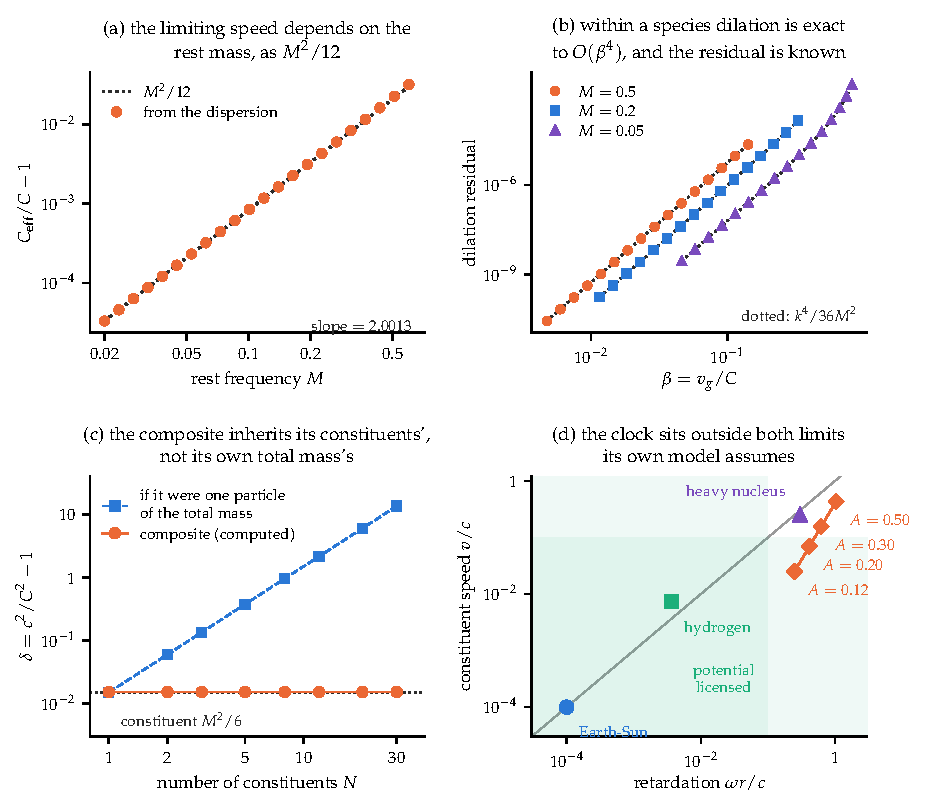
\includegraphics[width=\textwidth]{conearc.pdf}
\caption{The cone arc of Sections~\ref{sec:massivecone}--\ref{sec:potential},
computed. (a) The limiting speed extracted from the exact dispersion
tracks $M^2/12$; the fitted log--log slope is $2.0013$. (b) Using each
species' own $C_{\rm eff}$, the free mass-shell diagnostic has an
$O(\beta^4)$ residual that follows
the analytic $k^4/36M^2$ (dotted)
to within $1.1\%$ across three masses. (c) The free-threshold result: the
normalized cone shift $E_{\rm thr}(0)E_{\rm thr}''(0)/C^2-1$ at the bottom
of an identical-particle continuum is constant to seven digits as the
particle number runs $1\to30$, while treating the total mass as one particle
grows as $N^2$. This is not a bound-state result. (d) The two limits hidden in a
distance potential, with real systems placed. Orbits lie on the diagonal
because $\omega r = v$ for them; the mechanical clock does not, and sits
outside the licensed corner on both axes --- more relativistic internally
than a heavy nucleus.}
\label{fig:conearc}
\end{figure}

\subsection{The discrete diagnostic}
\label{sec:diagnostic}

The obligations above were all continuum-shaped: a cone, a boost, a
dispersion. A discrete substrate admits one further test that has no
continuum analogue, and it is worth recording even though it decides
nothing here.

If a theory supplies a coarse-graining from its histories to locally
finite causal sets, the recursion \eqref{eq:recursion} becomes accretion
of one event at a time onto a partial order, and covariance acquires a
discrete form: the probability of reaching a given unlabelled causal set
must not depend on the labelled growth path,
$\prod_{r\in\gamma}t_r = \prod_{r\in\gamma'}t_r$. Under internal
temporality, Markov normalization, discrete general covariance
\emph{and Bell causality}, the classical solutions are
classified~\cite{rideoutsorkin}; the quantum case remains an open
programme~\cite{sorkin,srivastavasurya}. Two precision points are worth
carrying: the birth label of an element is gauge, whereas the stage
number $n = |C_n|$ is label-invariant and is not gauge, though neither is
it a coordinate time. We record this as an \emph{optional diagnostic}: it
is neither necessary nor sufficient for hiding a preferred lattice, and
it does not replace the Lorentz-recovery obligation above.

The division leaves a bill: the one-body half closed with numbers, the
two-body half open, priced, and gated on an instrument this paper costed
in Section~\ref{sec:clock} and the substrate did not supply. The next
section observes that the architecture's own stage index is gated the
same way --- which is the promise left standing in
Section~\ref{sec:succession}.

% =====================================================================
\section{Quantum gravity, and the clock again}
\label{sec:qg}

Canonical quantization of generally covariant general relativity yields
the Hamiltonian constraint and the familiar problem of time,
schematically $\hat{H}\Psi = 0$~\cite{dewitt}. The standard
relational repair conditions on a clock subsystem~\cite{pagewootters},
recovering evolution as conditional potentiality, with known objections
about localization and propagators~\cite{kuchar} that are partly
addressed by covariant clock observables~\cite{hohn} and complicated
again for finite-resource clocks~\cite{hausmann}.

For this paper the point is structural and closes a loop. The v2 contract
keeps three quantities separate:
\begin{equation}
 \begin{aligned}
 n& &&\text{ontic global update order},\\
 \phi_x(n),\tau_x& &&\text{local phase and operational duration},\\
 k_x& &&\text{compliant actualization-gate count}.
 \end{aligned}
\end{equation}
The first is postulated and does not need to be read from a clock. The second
turns succession into operational duration and must be carried and maintained
inside the history. The third counts only fixed-phase crossings that pass the
clock-compliance tolerances. For the selected quartic carrier
$TA=\sqrt\pi G^*\sqrt{m/(2\lambda)}$: $G^*$ fixes the cadence of eligibility,
not the global order and not the outcome. \textbf{The clock programme is
therefore the precondition of local duration and gating, not the source of
the world's global update index.}

One further hypothesis class connects gravity to $\Sigma$ directly, by
making the gravitational self-energy difference set an actualization
timescale, $\tau \sim \hbar/E_G$~\cite{diosi,penrose}. Its
parameter-free version is excluded by underground radiation
tests~\cite{donadi}, and the Markovian model is further constrained by
XENONnT~\cite{xenon}. We note the structural resemblance to
Section~\ref{sec:born}'s slow-channel result --- a gravitational sector
supplying the slow gate --- and we label it exactly as what it is: a
speculative alignment between two independently derived shapes of
requirement, not evidence for either.

That closes the loop the construction opened. The v2 reference pipeline now
runs the directed composition
$n\to$ substrate history $\to\omega\to$ local instruments $\to G^*$ gate
$\to\Sigma\to$ records, with the controller audit carried alongside it.
Because its preparation map and Born weights are adopted, it is a standalone
mathematical consistency model, not a physical substrate realization. The
older side-by-side check below remains useful only as an independent-module
audit.

% =====================================================================
\section{A side-by-side minimal demonstrator}
\label{sec:toy}

The preceding sections established their results one instrument at a
time. A smaller bookkeeping question remains: can their declared modules
be evaluated at one parameter set without a transcription contradiction?

This section records substrate, clock, register, gate, and noise
calculations in one computable artifact, small enough to run in under a
minute. Three identities can be checked to machine precision. It is a
side-by-side demonstrator, not an instrument of record: no claim of
Sections~\ref{sec:clock}--\ref{sec:born} depends on it, and it establishes
no composed physics.

The modules in this older artifact are independent computations: no module
consumes another's state, and there is no feedback anywhere in it. The test
catches shared-constant and transcription inconsistencies; it does not show
that the mechanisms coexist in one dynamical system. Separately, the v2
reference simulator composes history, preparation, instruments, maintained
gate, selector, and records through explicit interfaces. It still imports the
state--effect weights and does not implement physical register-to-carrier
backreaction, so a substrate-native coupled model remains open.

\begin{figure}[p]
\centering
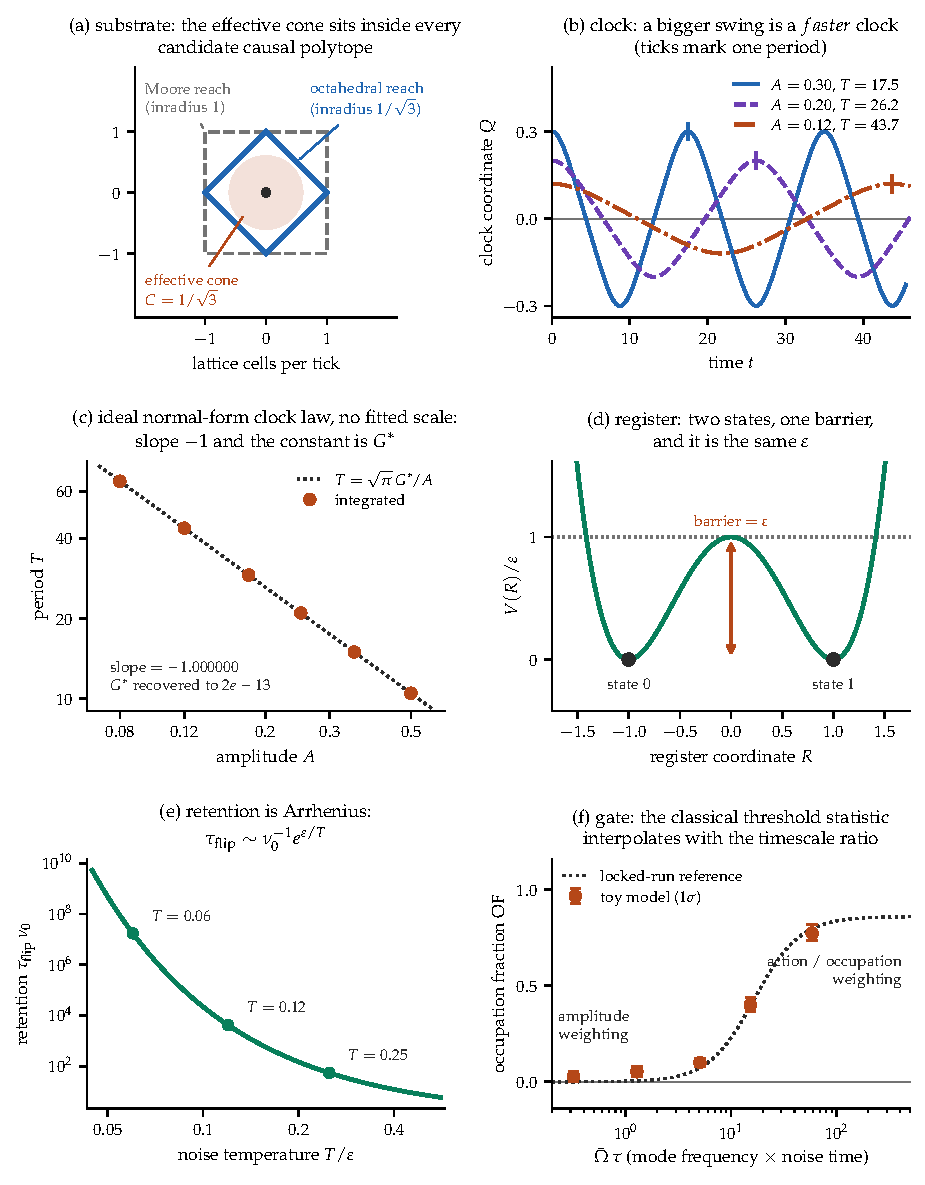
\includegraphics[width=\textwidth]{toymodel.pdf}
\caption{Six minimal temporal-interior modules, computed side by side but
not dynamically coupled. (a) The effective cone lies inside the strict
reach. (b,c) The ideal quartic normal form has $T\propto A^{-1}$ and
recovers $G^*$ to $1.6\times10^{-13}$ without a fitted scale; this does not
make the full carrier exactly quartic. (d,e) The compact-support register's
barrier equals its well depth and gives the Arrhenius estimate under the
stated Kramers assumptions. (f) The
classical threshold statistic moves from amplitude toward
action/occupation weighting as $\bar\Omega\tau$ grows; bars are $1\sigma$
bootstrap intervals and the dotted curve is the locked-run descriptive
reference of Figure~\ref{fig:bornregime}.}
\label{fig:toymodel}
\end{figure}

\subsection{The ideal normal-form clock law, exactly}

The carrier's mirror-even mode reduces at leading quartic order to
$m\ddot Q = -4\lambda Q^{3}$. Energy conservation gives
$\tfrac{m}{2}\dot Q^{2} + \lambda Q^{4} = \lambda A^{4}$, so a quarter
period is
\[
\frac{T}{4} \;=\; \frac{1}{A}\sqrt{\frac{m}{2\lambda}}
\int_{0}^{1}\!\frac{du}{\sqrt{1-u^{4}}}
\;=\; \frac{1}{A}\sqrt{\frac{m}{2\lambda}}\cdot\frac{\sqrt{\pi}\,G^{*}}{4},
\]
using $\int_{0}^{1}(1-u^{4})^{-1/2}\,du = \tfrac14 B(\tfrac14,\tfrac12)$.
Hence the ideal normal-form period law
\begin{equation}
T\cdot A \;=\; \sqrt{\pi}\,G^{*}\,\sqrt{\tfrac{m}{2\lambda}},
\qquad G^{*} = \Gamma(1/4)/\Gamma(3/4).
\label{eq:periodlaw2}
\end{equation}

Panel~(b) of Figure~\ref{fig:toymodel} shows this without any rescaling:
the three trajectories have $A = 0.30, 0.20, 0.12$ and periods
$17.5, 26.2, 43.7$. Panel~(c) integrates six amplitudes spanning a factor
of six at tolerance $10^{-12}$, locates each far turning point by event
detection, and recovers a fitted log--log slope of $-1.000000000$ and
$\max_{A}\lvert G^{*}_{\rm rec}/G^{*} - 1\rvert = 1.61\times10^{-13}$,
where $G^{*}_{\rm rec}$ inverts \eqref{eq:periodlaw2} with no free
parameter. The recovery sits at integrator tolerance, which is the correct
outcome for an identity rather than a fit.

The significance is the contrast, not the constant. A quadratic well
would give $\pi$ and isochrony; the quartic well gives $G^{*}$ and
amplitude dependence. That is the difference between a clock whose rate is
independent of how hard it was struck and one whose rate is not --- and it
is the reason Section~\ref{sec:clock} treats the lemniscatic clock as a
purchase rather than a gift.

\subsection{Testing the one-constant, three-role claim}

The architecture's economy claim is that a single energy scale prices
three apparently unrelated things: the depth of the well that binds the
carrier, the quartic stiffness $\lambda$ that sets the clock rate through
\eqref{eq:periodlaw2}, and the Arrhenius barrier in $\tau_{\rm
flip}\nu_{0}\sim e^{\varepsilon/T}$. The commitment is that these are not
three independent constants.

\emph{The demonstrator exhibits two of the three, not all three.} In the
script, $\varepsilon$ is set once and drives the register well and the
retention curve --- panels~(d) and~(e), where the barrier is the well
depth with no geometric prefactor and retention runs from $\sim\!55$
attempt times at $T = 0.25\,\varepsilon$ to $\sim\!1.7\times10^{7}$ at
$T = 0.06\,\varepsilon$. The clock panel integrates its own stiffness as
an independent hard-coded value, and the detector its own threshold and
noise width. So the third role --- $\varepsilon$ \emph{setting} the clock
rate --- is asserted by the architecture and \emph{not} exhibited here.
Nor could this instrument exhibit it: $\Gstar$ is recovered from
\eqref{eq:periodlaw2} in a form independent of $\lambda$, which is what
makes the recovery a clean test of the law and a null test of the
coupling.

\emph{And the economy claim, pressed, does not hold.} The clock's
stiffness is $\lambda_{\rm eff}=8k_1k_2/(k_1+3k_2)$. Here $k_1$ and
$k_2$ are \emph{radial} curvatures. For the registered law
\eqref{eq:registerbond}, $k_1=96\varepsilon$. If the purchased closure is
declared to have the same shape stretched to radial range $3r_0$, its
argument is $q/9$, its depth is an independent $\varepsilon_2$, and
$k_2=\tfrac{32}{3}\varepsilon_2$. Writing
$\rho=\varepsilon_2/\varepsilon$,
\begin{equation}
\lambda_{\rm eff} = \frac{256\,\varepsilon\,\rho}{3+\rho},
\qquad
\Delta E = \varepsilon,
\qquad
\ln(\tau_{\rm flip}\nu_0) = \varepsilon/T .
\label{eq:economy}
\end{equation}
Two things follow, and both correct the claim as it was stated. First,
the three responses do not move in fixed proportion even at fixed $\rho$:
their exponents in $\varepsilon$ are $+1$ for the barrier, $+1$ for the
log-retention and $-\tfrac12$ for the clock period, so raising
$\varepsilon$ deepens the well, lengthens the memory exponentially and
\emph{speeds} the clock. Second and more seriously, $\rho$ is a free
dimensionless parameter that appears in the clock and in neither of the
others: sweeping $\rho$ from $\tfrac14$ to $16$ moves $T\!\cdot\!A$ by a
factor of $3.3$ while the barrier and the retention law are untouched.
That is precisely the falsifier this subsection wrote for itself --- a
measurement moving one of the three without the others --- and it is
fired not by an experiment but by the second interaction species that
Section~\ref{sec:mvc} had already purchased and priced. \textbf{There is
a separate clock constant, and its name is $\rho$.}

What survives is the leading-normal-form statement. In the $A\to0$
quartic normal form, $\Gstar$ does not depend on $\rho$: integrating that
reduced mode across
$\varepsilon\in[\tfrac12,2]$ and $\rho\in[\tfrac14,4]$ recovers
$T\!\cdot\!A\sqrt{2\lambda_{\rm eff}/m}/\sqrt\pi = \Gstar$ to
$6\times10^{-14}$ throughout. Within that limit, the second energy scale
buys the clock's \emph{rate} and cannot touch the normalized quartic
coefficient. Finite-amplitude compact-bond motion remains unsimulated, as
Section~\ref{sec:mvc} states. The economy claim fails where it priced the
rate and survives only at leading normal-form order where it priced the
number.

\subsection{The regime, on an independent instrument}

Panel~(f) reruns the weighting question with a different construction from
the one behind Figure~\ref{fig:bornregime}. Two standing modes carry
lattice-dispersion frequencies $\Omega(k) = 2\arcsin(C\sin(k/2))$ and are
given \emph{equal action}, $A_{2} = A_{1}\sqrt{\Omega_{1}/\Omega_{2}}$, so
they differ in amplitude but not in occupation. The two candidate
weightings then predict opposite values for the ratio of second-harmonic
coefficients in the excess crossing rate, and the occupation fraction
$\mathrm{OF} = (R - R_{\rm amp})/(1 - R_{\rm amp})$ is $0$ and $1$
respectively by construction.

\begin{center}
\small
\begin{tabular}{@{}rlr@{}}
\toprule
$\bar\Omega\tau$ & OF ($1\sigma$ bootstrap) & reference \\
\midrule
0.32  & $0.028\ (-0.026/{+}0.028)$ & 0.000 \\
1.28  & $0.052\ (-0.027/{+}0.027)$ & 0.005 \\
5.07  & $0.100\ (-0.023/{+}0.021)$ & 0.073 \\
15.22 & $0.400\ (-0.034/{+}0.039)$ & 0.393 \\
58.77 & $0.774\ (-0.041/{+}0.047)$ & 0.796 \\
\bottomrule
\end{tabular}
\end{center}

\noindent The two upper cells agree closely with the locked-run reference;
the lower cells sit high by about one standard deviation, which is what a
deliberately small instrument looks like when its uncertainty is reported
rather than hidden. The qualitative structure --- amplitude weighting
below the crossover, occupation weighting above it --- reproduces on an
instrument that shares no code path with the protocol-locked scan.

None of this promotes the detector result into a Born law. The mechanism
class is still declared, the ensemble is still imposed, and the engine's
own cells still sit at $\bar\Omega\tau \in [0.19, 0.86]$, below the
crossover, which is why Section~\ref{sec:born} reports a null there. What
the model shows is narrower and worth stating plainly: the interpolation
is not an artefact of one instrument's construction.

\subsection{The causal cell in three dimensions}
\label{sec:cell3d}

Panel~(a) of Figure~\ref{fig:toymodel} is drawn in the plane for
legibility. Developed properly in three dimensions it yields the paper's
sharpest distinction between exact dependency support and a long-wave
propagation scale, and it is worth stating on its own.

\begin{figure}[p]
\centering
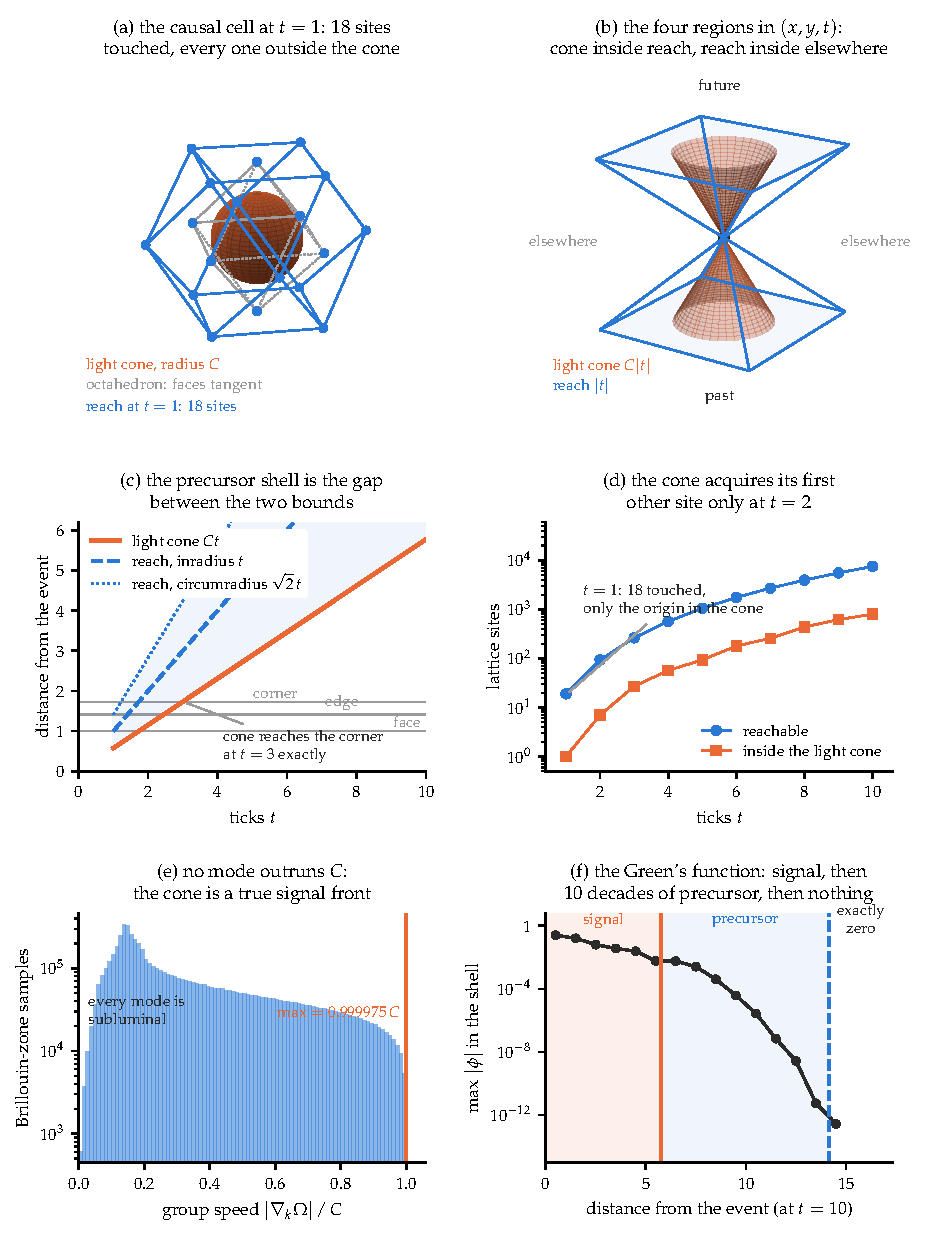
\includegraphics[width=\textwidth]{causal3d.pdf}
\caption{The causal bookkeeping partition around one event. (a) At $t=1$ the
effective-cone sphere is inscribed in the octahedron --- its inradius
\emph{is} $C$, so the eight faces are tangent --- which is itself inside
the reach polytope. (b) Past, future, and elsewhere in $(x,y,t)$, with the
round cone strictly inside the square-sectioned reach. (c) The precursor
shell is the gap between the two bounds; the cone closes over the body
diagonal at $t=3$ exactly. (d) At $t=1$ eighteen sites have been touched
and only the origin lies in the effective cone. (e) The $181^3$ scan finds
no sampled group velocity above $C$; this supports an effective cone but is
not a proof of the global supremum. The strict front is the reach boundary.
(f) Across the shell the Green's function falls ten decades and then
terminates in an exact zero.}
\label{fig:causal3d}
\end{figure}

Two structures compete to define causal reach, and they do not coincide.
\emph{Reach} is unconditional: the update rule touches a finite neighbour
set each tick, so after $t$ ticks the field is exactly zero outside the
$t$-fold dilation of the causal polytope. This is locality, not dynamics.
\emph{The effective cone} is dynamical: long-wave packet peaks propagate
at asymptotic speed $C$. Between the two surfaces sits a shell that is
formally reachable but outside that cone. It is useful to track this as a
fourth bookkeeping region, but it is not unique to discreteness:
dispersive continuum systems also carry precursors outside a group-velocity
cone.

The geometry at one tick is exact, and contains one coincidence that is
not a coincidence. The octahedron's inradius is $1/\sqrt3$, which is the
cone speed; the effective-cone sphere is therefore \emph{inscribed} in the
octahedron, tangent at its eight faces, and the octahedron is in turn
inside the cuboctahedron (inradius $1$) and the cube (inradius $1$). This
is what $C = \min\{\text{containment bounds}\}$ means geometrically: the
cone fits inside every candidate causal polytope, and fits the tightest
one exactly.

The census is then startling at first reading. \textbf{At $t=1$ the
effective cone contains exactly one lattice site --- the origin --- while eighteen
have already been touched.} The nearest site is at distance $1$; the cone
has radius $0.577$. The cone acquires its first other site at $t=2$, and
at $t=3$ it contains exactly the twenty-seven-site block, because
$3C = \sqrt3$ is precisely the body-diagonal distance. The correct reading
is not that causality fails at one tick, but that the effective-cone sphere
contains no non-origin lattice site until the second tick.

What occupies the shell is characterized at the resolution studied by two
measurements. First, the group velocity of the leapfrog was differentiated
analytically and evaluated on a $181^3$ grid of the Brillouin zone. The
scan found no value above $C$ and approached $C$ as $k\to0$; it is evidence
for, not a proof of, the global supremum. This does \emph{not} make $C$ the
signal front: a supremum over group velocities bounds where the
disturbance is \emph{concentrated}, not where it is exactly zero, and the
next measurement shows the field is nonzero outside $Ct$. The strict
front is the reach boundary; $C$ is the effective cone. Second, the
point-source Green's function at
$t=10$ falls from $5.8\times10^{-3}$ at the cone to $2.8\times10^{-13}$ at
the support boundary --- ten decades, about $1.3$ per lattice cell --- and
is then identically zero by the finite-support update rule. In that run the
shell profile is precursor-like and falls approximately exponentially
across the sampled cells. No uniform exponential bound over time and
direction is proved.
Figure~\ref{fig:causal3d} draws the whole structure --- the cone inside
the reach polytope, the census by tick, and the ten-decade fall to that
exact zero.

The cuboctahedral exact support is a structural property of this update;
the distinction between support and a group-velocity cone is not unique to
discrete systems. In the reported runs the detected contour is much more
isotropic than the stencil and its residual anisotropy decreases as a
power of elapsed time. Whether that is phenomenologically adequate is not
established here.

So the artifact places the calculations in one program and catches a real
failure of the advertised constant economy. It does not couple the modules
or show them coexisting as one physical system. Nor can it say which
pillar supplies which layer, and which layer nobody supplies. That is the
statement the next section owes.

% =====================================================================
\section{The merge, stated exactly}
\label{sec:synthesis}

We can now say what merges. Figure~\ref{fig:merge} states it as a supply
diagram: which pillar supplies which layer of the architecture, and which
layer nobody supplies.

\begin{figure}[t]
\centering
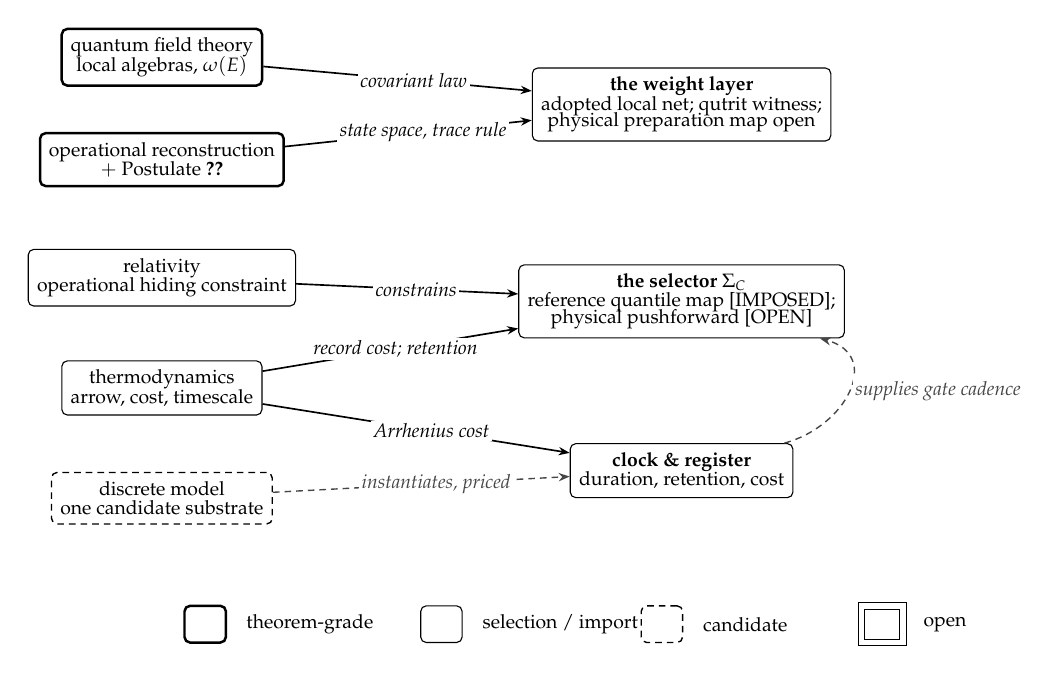
\begin{tikzpicture}
% ---- sources (left) -------------------------------------------------
\node[thm]  (qft)  at (0,2.05)  {quantum field theory\\[-1pt]\figsub local algebras, $\omega(E)$};
\node[thm]  (rec)  at (0,0.75)  {operational reconstruction\\[-1pt]\figsub $+$ Postulate~\ref{post:B}};
\node[sel]  (rel)  at (0,-0.75) {relativity\\[-1pt]\figsub operational hiding constraint};
\node[sel]  (thm2) at (0,-2.15) {thermodynamics\\[-1pt]\figsub arrow, cost, timescale};
\node[conj] (mod)  at (0,-3.55) {discrete model\\[-1pt]\figsub one candidate substrate};

% ---- architecture layers (right) ------------------------------------
\node[sel]   (W) at (6.6,1.45)  {\textbf{the weight layer}\\[-1pt]\figsub
   adopted local net; qutrit witness;\\[-2pt]\figsub physical preparation map open};
\node[sel] (S) at (6.6,-1.05) {\textbf{the selector} $\Sigma_C$\\[-1pt]\figsub
   reference quantile map [IMPOSED];\\[-2pt]\figsub physical pushforward [OPEN]};
\node[sel]   (C) at (6.6,-3.20) {\textbf{clock \& register}\\[-1pt]\figsub
   duration, retention, cost};

\draw[con] (qft)  -- node[lbl,pos=0.56] {covariant law} (W);
\draw[con] (rec)  -- node[lbl,pos=0.56] {state space, trace rule} (W);
\draw[con] (rel)  -- node[lbl,pos=0.54] {constrains} (S);
\draw[con] (thm2) -- node[lbl,pos=0.52] {record cost; retention} (S);
\draw[con] (thm2) -- node[lbl,pos=0.55] {Arrhenius cost} (C);
\draw[wk]  (mod)  -- node[lbl,pos=0.55] {instantiates, priced} (C);
% the clock supplies local gate cadence, not the global update index
\draw[wk]  (C) to[out=15,in=-15,looseness=1.5]
  node[lbl,pos=0.5,right=1pt] {supplies gate cadence} (S);

% ---- shape legend ---------------------------------------------------
\begin{scope}[shift={(0,-5.15)}]
  \node[thm]   (l1) at (0.55,0) {\phantom{Xy}};
  \node[sel]   (l2) at (3.55,0) {\phantom{Xy}};
  \node[conj]  (l3) at (6.35,0) {\phantom{Xy}};
  \node[openb] (l4) at (9.15,0) {\phantom{Xy}};
  \node[font=\figsub, anchor=west] at (0.95,0) {theorem-grade};
  \node[font=\figsub, anchor=west] at (3.95,0) {selection / import};
  \node[font=\figsub, anchor=west] at (6.75,0) {candidate};
  \node[font=\figsub, anchor=west] at (9.55,0) {open};
\end{scope}
\end{tikzpicture}
\caption{What supplies what. Shapes encode status, never colour, as shown
in the legend: solid for theorem-grade within stated premises, thin for
selections and imported representations, dashed for a candidate
instantiation, and double-ruled for an open interface. Other open
interfaces are labelled explicitly in the nodes and caption. Solid arrows
are constructions; the dashed arrow marks a candidate instantiation that
is priced rather than free. The abstract local net and qutrit witness are
adopted at different scopes. Singular actuality and the contextual quantile
selector are imposed; the selector proves exact reference pushforward but
does not recover physical Born/Bell frequencies.}
\label{fig:merge}
\end{figure}

\textbf{Quantum field theory supplies a covariant comparator for the
potential layer [IMPORTED].} Local algebras, covariant evolution, and
spacelike order-independence are standard physics. V2 adopts an abstract
discrete local net and supplies a finite Type-I qutrit witness. Recovering its
preparation map and any physically relevant continuum representation from
substrate dynamics remains \textbf{open}.

\textbf{The reconstruction programme plus Postulate~\ref{post:B} supplies
trace-form weights conditionally [EXTERNAL THEOREM].} It does not construct
a physical substrate measure whose pushforward equals those weights. The
Born square is settled inside the imported effect space; the physical Born
pushforward remains \textbf{open}.

\textbf{Relativity constrains the selector, and prices each option.}
The reference ActualizationBatch has commuting local instruments and
remote-setting-independent marginals. It does \emph{not} establish empirical
hiding of the preferred tick: the gap between \eqref{eq:R3} and
\eqref{eq:R4} remains a physical recovery debt.

\textbf{Singular actuality supplies one record [IMPOSED].} Unselected
alternatives are potential or counterfactual relative to that record, not
additional actual histories. Identifying the model's manifestation rule
with the selector is a priced conjecture, not a theorem.

\textbf{Thermodynamics supplies the record bill, not the statistics.} The
implemented update is operationally lossy and the register has a priced
retention time. A complete entropy and reset account is open. None of these
facts determines the relative frequencies of alternative records.

\textbf{Bell supplies an independent cross-context obstruction [THEOREM].}
One common substrate space carrying four jointly defined local response
variables under one setting-independent ensemble measure implies
$|S|\le2$, however singular, dissipative, or noninvertible each record is.
The imposed reference selector explicitly rejects joint local response
factorization while preserving measurement independence; it reaches the
selected quantum correlations only because it consumes their weights.

\textbf{The discrete model instantiates the architecture and prices it.}
It supplies succession, a strict dependency reach, screened harmonic
clock candidates, and candidate manifestation events. It currently
realizes the leading-order lemniscatic clock only in the purchased
construction; no native quartic clock has been found. Retention likewise
requires the declared register and bath assumptions. The slow-channel
experiment supplies only a classical detector regime.

The merge is therefore an itemized architecture, not a unification:
quantum theory specifies conditional weights, thermodynamics prices the
production and retention of a record, relativity constrains its operational
description, and the reference selector shows that deterministic contextual
actualization is logically compatible with the Bell accounting. The central
open object is the joint \emph{physical} construction of the preparation map,
equilibrium measure, response map, and required Born/Bell pushforwards without
reading their targets.

Itemized is a claim that can be checked, and checking it needs the items
in one place at their actual strength rather than at the strength the
surrounding prose lends them. That table is next, and it is the only part
of this paper that binds.

% =====================================================================
\section{Status of claims}
\label{sec:ledger}

Table~\ref{tab:ledger} states every substantive claim in the paper at its
actual strength. Where the body and this table disagree, the table is
correct.

{\small
\renewcommand{\arraystretch}{1.05}
\begin{longtable}{p{0.46\textwidth} p{0.46\textwidth}}
\caption{Every substantive claim in the paper, at its actual strength.}\label{tab:ledger}\\
\toprule
\textbf{Claim} & \textbf{Status} \\
\midrule
\endfirsthead
\multicolumn{2}{@{}l}{\footnotesize\itshape Table \thetable, continued}\\[2pt]
\toprule
\textbf{Claim} & \textbf{Status} \\
\midrule
\endhead
\bottomrule
\endfoot
The actual/potential distinction \eqref{eq:distinction} &
\textbf{[AXIOM --- semantic primitive]}; organizes the scaffold but
supplies no dynamics or frequencies \\
Singular actuality & \textbf{[IMPOSED --- Postulate~\ref{post:A}]}; one
mutually exclusive outcome enters the record; not derived from the model
\\
Unselected alternatives remain potential/counterfactual & True by
definition within the scaffold; no theorem that they persist as independent
substrate objects \\
Closure map $\Gamma$ from history to state & Declared scaffold; history
alone is insufficient \\
Actual record algebra \eqref{eq:actualalgebra} & \textbf{[AXIOM]}; bounded
classical configuration functions are commutative and finite ternary records
form $\mathbb C^{3^{|\Lambda|}}$, not a full matrix algebra \\
Potentiality net and qutrit witness \eqref{eq:qutritnet} & \textbf{[AXIOM]
+ [SELECTED REFERENCE REPRESENTATION]}; finite regions are Type~I and the
quasi-local reference limit is UHF. No automatic Type-III claim \\
Preparation map $\Gamma_\Lambda$ & Adopted interface with restriction
consistency proved in the reference witness; physical substrate recovery
\textbf{[OPEN]} \\
Identification of genesis/manifestation with $\Sigma_O$ &
\textbf{[CONJECTURE --- model-scoped identification]}; the engine rule is
explicit, but no laboratory outcome map is constructed \\
Genesis readout is many-to-one & \textbf{[MEASURED --- engine-scoped]};
distinct flux magnitudes yield the same discrete record while the
continuous flux remains stored \\
Complete update-map noninjectivity & \textbf{[THEOREM --- current-engine
scope]}; witnessed by evaporation, not by genesis alone and not for every
event \\
Resource price of the candidate record & \textbf{[MEASURED] + [THEOREM]};
in the declared model, accepted genesis has a positive drain, and a reusable
symplectic energy lift requires added record-bearing bath variables plus
reset, replacement, export, or feedback. No universal energy quantum or
complete Landauer cycle is derived \\
Operational framework and six principles & Imported premises; not derived
here \\
Complex finite-dimensional quantum theory & External theorem, conditional
on those premises~\cite{cdp} \\
Convex state/effect structure & Derived within the imported framework \\
Effect-noncontextual additivity & Declared postulate
(Post.~\ref{post:B}) \\
Trace rule and the Born square \eqref{eq:born} & External
\textbf{[THEOREM]}, conditional on the imported effect space and
Postulate~\ref{post:B}~\cite{busch} \\
Discrete local-net proof package & \textbf{[THEOREM --- adopted reference
net]}; isotony, actual commutativity, spacelike commutation, compatible state
restriction, normalized causal instruments, and order independence \\
Physical Born pushforward \eqref{eq:pushforward} & \textbf{[OPEN]};
neither the physical response map nor its ensemble measure is constructed
\\
Deterministic quantile selector \eqref{eq:quantileselector} &
\textbf{[IMPOSED REFERENCE REALIZATION]}; exact pushforward under invariant
Lebesgue measure, measurement independent and globally contextual. It consumes
$\omega(E)$ and is therefore not a physical Born derivation \\
CPTP dynamics, unitarity, Schr\"odinger form & External theorems,
conditional on their stated premises \\
Quadrature root $\times$ degree ratio \eqref{eq:qrdr} & Exact identity
within the homogeneous family $V=\lambda|x|^n$; it is not a universal
factorization for arbitrary mechanical potentials. The harmonic case is
uniquely self-reproducing within that family \\
Threshold forcing (Prop.~\ref{prop:threshold}) & Exact within H1--H4 and
only as $A\to0$. It neither places a substrate at the codimension-one
threshold nor proves finite-amplitude quarticity \\
Finite-amplitude clock drift & The sextic family
\eqref{eq:sexticdrift} is exact for that family. An exploratory
harmonic-spring surrogate gives $+0.33\%$: its reduced quadrature assigns
$+0.314\%$ to amplitude-dependent mass and $+0.014\%$ to potential at
$A=0.12$. No compact-law finite-amplitude result is supplied \\
\textbf{$\Gstar$ is chosen, not derived} & No valid relativistic carrier
has produced it. The native screen was negative; the purchased four-body
carrier is only asymptotically quartic and Galilean; the soliton
shape-mode evidence is
unreproduced and isochronous \\
The rigidity trichotomy and buckling criterion & Exact within their
declared mechanical model and hypotheses \\
Minimum viable leading-order quartic carrier & Minimal four-body/two-scale
construction and $A\to0$ normal form exact. Finite-amplitude numbers come
only from a curvature-matched harmonic surrogate; $\Gstar$ recovered to
$2\times10^{-6}$ there only by extrapolation. Galilean and disqualified as
a relativity test \\
No native quartic clock & Negative at screened scope only; not a no-go
theorem \\
Context-blind dual clock feedback and compliant gate & \textbf{[SELECTED
REFERENCE CONTROLLER]}; detuning and amplitude/action channels with explicit
work, dissipation, and compliance audit. Native actuation and non-rescalability
remain \textbf{[OPEN]} \\
Register barrier $=\varepsilon$ (Prop.~\ref{prop:registerbarrier}) &
\textbf{[THEOREM --- declared compact-support model]}; exact plane crossing
and $N\le2$ bound plus $11{,}250{,}000$ exact-rational,
outward-rounded boxes, zero samples and zero uncertified. Conditional on
compact support; a Morse/LJ tail lowers the barrier \\
One constant, three roles & \textbf{Refuted as stated.}
$\rho=\varepsilon_2/\varepsilon$ moves the clock rate alone; in the
leading $A\to0$ quartic normal form, $\Gstar$ is independent of $\rho$ to
$6\times10^{-14}$. No finite-amplitude compact-law result \\
Threshold interpolation toward action/occupation weighting &
\textbf{[MEASURED --- mechanism-scoped, imposed ensemble]}; OF is a
regression coordinate, not a probability. Neither an exact Born law nor a
substrate theorem \\
Non-transfer to the model's thermal field & Protocol-locked negative at
sampled scope; same-band diagnosis post-hoc \\
Purity requirement & Measured on five shares/32 seeds in one declared
additive instrument; not a universal proposition \\
Slow sector is slow ($\tau=317.9$ vs $0.81$) & Measured profile; deterministic,
so seed-independence is vacuous \\
Common-measure CHSH bound (Prop.~\ref{prop:irreversiblebell}) &
\textbf{[THEOREM]}; four jointly defined responses under one
setting-independent measure imply $|S|\le2$. Record invertibility and
energetic cost are not premises \\
Singularity, dissipation, or noninvertibility \emph{alone} as an escape
from Fine/Bell &
\textbf{[CLOSED NEGATIVE]}; it changes record formation, not the induced
joint distribution \\
Reference CHSH recovery by $\Sigma_C$ & \textbf{[THEOREM inside adopted
algebra + IMPOSED selector]}; selected singlet/observables give $2\sqrt2$,
all local marginals are no-signalling, local factorization fails, and PR-box
$S=4$ is excluded. No physical substrate Born/Bell recovery \\
Order-independence \eqref{eq:R3} $\nRightarrow$ equivariance
\eqref{eq:R4} & Logical separation; order independence passes in the adopted
causal-instrument reference model, while empirical preferred-order hiding and
strong history equivariance remain open \\
Operational hiding of a preferred foliation & Conditional reduction
(Prop.~\ref{prop:hiding}); follows if quantum composed-history statistics
and spacelike order-independence are already supplied \\
Free scalar spatial stencil & \textbf{[THEOREM --- tree level]}; unique
face/edge weights yield normalized isotropy through $O(k^4)$, with leading
directional residual $(ka)^4/3240$ \\
Radiative stability / dimension-four protection & \textbf{[OPEN ---
HARD]}; cubic symmetry does not relate temporal/spatial, electric/magnetic,
native-vector, or inter-sector coefficients. One frozen QED-like branch
requires a dimension-four counterterm; no on-shell closure is shown \\
Spatial rotational isotropy & Not closed generally. Only the declared
scalar spatial symbol is improved at tree level; the complete interacting
operator inventory remains open \\
Strict causal support of the M18 wave update & \textbf{[DERIVED]}; face and
edge sites are nonzero at $t=1$, corners zero. The support boundary is the
M18 reach polytope, not $Ct$ \\
Effective Green-function contours & \textbf{[MEASURED]}; near-$Ct$
threshold contour has $0.71\%$ anisotropy and sampled scaling
$t^{-1.1}$--$t^{-1.3}$. Not the exact causal surface or a uniform theorem
\\
Which neighbourhood defines causal reach & A model choice with exactly
distinguishable consequences; M6, M18 and M26 differ at the first tick.
Finite-run precursor suppression does not erase exact support \\
Free massive scalar modes & \textbf{[DERIVED --- toy sector]}; numerically
checked;
$C_{\rm eff}/C=1+M^2/12+\cdots$ and residual
$M^2\beta^4/4$. Electron/proton numbers are parametric evaluations, not
physical predictions \\
Free cross-sector symbol match & Exact integer-hop eighteen-square and
spatially cubic-covariant half-angle seven-square constructions. Half
offsets are therefore an economy, not an existence requirement. The latter
gives $n_{\rm cov}\le7$ but not a proven cubic-covariant minimum;
mixed-sector five/six remain unexcluded. A non-covariant four-square
numerical candidate has residual $5.3\times10^{-15}$ but no exact/interval
certificate, so the rigorous bounds are $3\le n_{\min}\le7$. A working matter sector, time discretization and
interactions are not built; current production sectors still mismatch.
If that economical half-offset construction is adopted, its ontology
remains \textbf{[OPEN]}: refined physical sites
recalibrate $a_{\rm phys}$, while staggered cochains keep $a$ but add
carrier types; neither reading is adopted \\
Free multiparticle-threshold inheritance & \textbf{[DERIVED --- FREE
THRESHOLD]}; \eqref{eq:freethreshold} and \eqref{eq:compweight} checked to
reported numerical precision. Not a bound-state or macroscopic theorem;
nucleon/Earth extrapolation withdrawn \\
Static-well composite clock & \textbf{[MEASURED --- exploratory,
inconclusive]}; the old $p=-1$ target used an infinitesimal-gap
approximation. Against the exact finite-gap comparator, six fixed cases at
$K=0.2$ differ by $0$--$1.1\%$; convergence and held-out-momentum controls
remain open \\
$\varphi^4$ soliton shape-mode clock & \textbf{[OPEN --- UNREPRODUCED; COMMON-CONE
MISMATCH]}; $p\simeq-1$ requires a fitted speed about $6\%$ below the
energy cone, and the committed runner does not reproduce the quoted campaign
\\
Interacting vertices, bound-state cones, composite boosts & \textbf{[OPEN]};
requires one interacting action, stress-energy, and boost generator \\
Gravitational actualization resemblance & Speculative alignment only;
the parameter-free version is externally excluded~\cite{donadi} \\
$\hbar$, Hamiltonian, masses, couplings & \textbf{Not derived} anywhere
in this paper \\
\end{longtable}}

\clearpage

% =====================================================================
\section{Open problems}
\label{sec:open}

\begin{enumerate}\itemsep3pt
\item \textbf{The Born pushforward for a concrete substrate.} Construct
$F_O$ and $\mu_{\rm eq}$ from the substrate's own dynamics without reading
target probabilities. The locked, unexecuted first campaign tests the
free-flux density $n=|\phi_+|^2$, equilibrium invariance, context overlap,
held-out instruments, and an explicit target-leak sentinel; interacting and
genesis transfer are later gates.
\item \textbf{The physical Bell pushforward.} V2 has already named the
rejected premise: the deterministic selector is globally contextual and
nonfactorizable, while measurement independence is retained. Recover that
response law from the substrate and show no-signalling on held-out contexts.
Noninvertibility, dissipation, and singular records do not answer this.
\item \textbf{Thermodynamic closure of record writing.} Complete a repeated
genesis--record--reset cycle with bath state, heat, work and entropy tracked.
The current bath-rank and nonrepeatability theorems price the missing
machinery but do not supply an autonomous cycle or a universal cost per
outcome.
\item \textbf{Native quartic timekeeping.} Does a finite integer
unit-strut tensegrity exist under the single-scale law, with blocking
form definite on its full flex space? No candidate realizes it; no
impossibility proof exists.
\item \textbf{What physically holds the threshold.} Proposition~\ref{prop:threshold}
forces the quartic \emph{at} $\mu = 0$, and $\mu = 0$ is a
codimension-one surface: the generic configuration is not on it, and an
unmaintained system falls off it and becomes a harmonic clock. The selected
dual feedback controller proves that a context-blind audited loop can hold the
reference clock. What native mechanism pays that work, survives held-out
perturbations, and distinguishes $G^*$ from a removable period rescaling?
\item \textbf{Shielded actualization.} The measured purity diagnostic
(page~\pageref{diag:purity}) indicates that, in the tested additive
instrument, the slow channel must be nearly
exclusive at the threshold. Can any physical manifestation rule be
shielded from its own field's fast noise?
\item \textbf{Preferred-order operational hiding.} Strong history
equivariance is not imposed by v2; its ontology permits a real preferred
order. Operational hiding is conditionally reduced by
Proposition~\ref{prop:hiding}, but the substrate Born/Bell hypothesis and
common-cone tests remain open.
\item \textbf{Quantum sequential growth.} The classical classification is
known; the quantum analogue with interfering weights is open.
\item \textbf{A physically coupled model.} The v2 standalone simulator now
composes history, preparation, local instruments, maintained $G^*$ gate,
selector, and records, but it imports the state--effect weights. Recover the
preparation and pushforward from substrate dynamics, add register-to-carrier
backreaction, and check the energy and signalling audits without target
leakage.
\item \textbf{What the second energy scale is.} $\rho =
\varepsilon_2/\varepsilon$ is now a named free parameter of the
architecture \eqref{eq:economy} rather than an unnoticed one. Either
derive it from the closure species' own structure, or accept it as a
second declared constant and price it in the import ledger.
\par\smallskip
\item \textbf{The barrier without compact support.} Proposition
\ref{prop:registerbarrier} is exact because the bond law vanishes
identically beyond $3/2$. Establish the corresponding statement for a
potential with a tail --- where the barrier is strictly below
$\varepsilon$ --- or show that compact support is forced.
\item \textbf{From the selected net to a physical representation.} The
finite qutrit witness is Type~I and its quasi-local limit is UHF. Determine
which preparation states the substrate generates, construct the relevant GNS
representations, and classify any limiting factor only from that
state-and-representation data. No Type-III status is assumed.
\item \textbf{Radiative and interacting common-cone matching.} Inventory
all symmetry-allowed operators of dimensions three and four for one action,
remove the single time-normalization redundancy, and compute the remaining
on-shell relative-cone eigenvalues. A required counterterm is imposed, not
emergent.
\item \textbf{Bound-state and soliton shape-mode recovery.} Compute $E_B(K)$ for a real
interacting bound state rather than the free threshold
\eqref{eq:freethreshold}. Separately restore a locked, reproducing soliton
shape-mode runner and test a comoving internal-mode projection, radiation and
finite-volume convergence, continuum scaling, and one independently fixed
shape-mode/energy cone on held-out velocities.
\end{enumerate}

% =====================================================================
\appendix
\section{Instruments, protocol records, and provenance}
\label{app:instruments}

Every measurement \emph{in the series catalogued below} has an
author-attested protocol record stating that outcomes, gates, kill
conditions, and runner hashes were fixed before execution. The current
hashes match those records, but the ordering is not corroborated by an
immutable external timestamp, as the next paragraph explains. The protocol
discipline still caught one invalid instrument: a mis-derived conservation
invariant failed at $3.6\times10^{-2}$ against a $10^{-10}$ tolerance, and
the instrument was re-locked and re-run before producing a reported number.

\paragraph{What that discipline does and does not currently establish.}
Stated plainly, because the distinction is easy to overclaim. The
recorded hashes verify that the runner in the repository \emph{now} is
byte-identical to the one the record names, and they do. What they do not
establish is the \emph{ordering}: the records and their runners entered
version control in commits made \emph{after} the runs they govern, and
the git tag that would have locked them beforehand --- a discipline this
project uses elsewhere, with $136$ such tags --- was never minted for
this arc. So pre-registration here is attested by the records' own dates
and an interim hash, not corroborated by an immutable external timestamp.
A reader who declines to take the dates on trust should treat these as
carefully documented analyses rather than as externally audited
pre-registrations. Separately and more seriously: the committed soliton
shape-mode runner does \emph{not} reproduce the parameter set quoted for
the shape-mode dilation campaign in Section~\ref{sec:oneenergy} --- it carries a superseded
first-pass configuration whose wider couplings lose the shape mode
entirely, and re-running it does not return the exponents printed there.
Those exponents should be read as unreproduced from the repository as it
stands until that runner is restored.

\begin{table}[h!]
\centering\small
\begin{tabular}{p{0.30\textwidth} p{0.26\textwidth} p{0.36\textwidth}}
\toprule
Instrument & Design & Outcome \\
\midrule
Weighting discrimination &
two modes, equal occupation, 48 seeds &
Regime-dependent: OF $0.024\to0.099$ \\
Saturation scan &
five arms, $\bar\Omega\tau = 0.64$--$78$ &
Approaches occupation endpoint: OF $\to0.836$, monotone \\
Engine regime map &
ten cells, native thermal field &
\textbf{No structure}: $|\rho|\le0.37 < 0.7$ \\
Slow-sector timescale &
self-gravitating configuration &
Slow: $\tau=317.9$ vs $0.81$, ratio $391$ \\
Slow-channel coupling &
five slow-shares, 32 seeds &
Instrument result: OF $=0.936$ at $f=1$ \\
\bottomrule
\end{tabular}
\caption{The Section~\ref{sec:born} instrument series. Full parameters,
seeds and gate values are in the corresponding protocol records; the exact
record--runner--hash mappings are printed below. The composed
model of Section~\ref{sec:toy} is deliberately \emph{not} listed: it is a
demonstrator that reproduces known answers, not an instrument of record,
and no claim in this paper rests on it.}
\end{table}

\paragraph{Exact protocol-to-runner mappings.}
The following are repository-relative paths; each SHA-256 is the current
runner hash that matches its named record. These mappings establish present
byte identity, subject to the ordering caveat above.

{\footnotesize\raggedright
\noindent\textbf{Weighting discrimination.}\quad
Record: \nolinkurl{docs/theory/10_eft_program/preregistrations/quantum_foundations/PREREG_BORN_DENSITY_UPCROSSING_v1.md}.\par
\noindent Runner: \nolinkurl{scripts/experiments/verify_born_density_upcrossing.py}.\par
\noindent SHA-256: \digest{269E3A2DA015A5515FA25C966BEC573A}{CF9F26408F8D7E0504BFB4CE8C60F690}.\par\smallskip

\noindent\textbf{Saturation scan.}\quad
Record: \nolinkurl{docs/theory/10_eft_program/preregistrations/quantum_foundations/PREREG_BORN_DENSITY_SATURATION_v2.md}.\par
\noindent Runner: \nolinkurl{scripts/experiments/verify_born_saturation_v2.py}.\par
\noindent SHA-256: \digest{2887218838B7B6D9A49F8EFF04617A82}{10CE7BB9B4096ED1F43E92E0DB283ED4}.\par\smallskip

\noindent\textbf{Engine regime map.}\quad
Record: \nolinkurl{docs/theory/10_eft_program/preregistrations/quantum_foundations/PREREG_BORN_REGIME_MAP_ENGINE_v1.md}.\par
\noindent Runner: \nolinkurl{engine/tests/campaign_born_regime_map.cpp}.\par
\noindent SHA-256: \digest{90DE28E7459458171154A41CD277A6E3F}{37586658A5A3063F4F3447438CD2EA7}.\par\smallskip

\noindent\textbf{Slow-sector timescale.}\quad
Record: \nolinkurl{docs/theory/10_eft_program/preregistrations/quantum_foundations/PREREG_LATENCY_SLOW_GATE_v1.md}.\par
\noindent Runner: \nolinkurl{engine/tests/campaign_latency_slow_gate.cpp}.\par
\noindent SHA-256: \digest{1F7B6AAC9D7F8C7BA935869B8A240F6D}{D51B2777BF036144E9D73FFB96EC6D82}.\par\smallskip

\noindent\textbf{Slow-channel coupling.}\quad
Record: \nolinkurl{docs/theory/10_eft_program/preregistrations/quantum_foundations/PREREG_LATENCY_SLOW_GATE_v1.md}.\par
\noindent Runner: \nolinkurl{scripts/experiments/temporal_interior/verify_latency_gate_mechanism.py}.\par
\noindent SHA-256: \digest{1E58D24D1F92F88E197FD16C779DE1F5}{D1462BAE9C4E8228D9FDF8F822B59F0D}.\par
}

\paragraph{Analytic artifacts, which are proofs rather than instruments.}
Three results in this paper are established by argument and verified by
computation rather than measured, so they carry no pre-registration and
belong outside the series above. All three run in seconds and print their own
assertions. Proposition~\ref{prop:registerbarrier}, both bounds, is
\texttt{scripts/experiments/temporal\_interior/}\allowbreak
\texttt{derive\_register\_barrier\_lower\_bound.py}; the economy result
\eqref{eq:economy}, including the exponents and the $\rho$-independence
of $\Gstar$ to $6\times10^{-14}$ in the leading $A\to0$ quartic normal
form, is
\texttt{derive\_epsilon\_economy.py} in the same directory. The period
decomposition of Section~\ref{sec:quadrature} is
\texttt{derive\_period\_decomposition.py}.

\paragraph{Exploratory clock provenance --- not pre-registered.}
The finite-amplitude harmonic-spring surrogate values in
Section~\ref{sec:clock} come from the following artifacts:

{\footnotesize\raggedright
\noindent Analysis: \nolinkurl{docs/theory/10_eft_program/native_time_carrier_programme/ANALYSIS_MINIMUM_VIABLE_CLOCK_CARRIER_v1.md}.\par
\noindent Runner: \nolinkurl{scripts/experiments/mvc_fourchain_clock.py}.\par
\noindent Current runner SHA-256:\par
\noindent\digest{E2AEAE0B73D311113F7944D053AD8AD1}{AD5E0AF2567687F9F7B321921E80F789}.\par
}
This is explicitly exploratory and \textbf{not pre-registered}.
\nolinkurl{dissemination/papers/semantic_ontology/figures/make_figures.py}
transcribes the reported $2\times10^{-6}$ and $3.3\times10^{-3}$ plotting
values; it does not recompute that surrogate campaign.

\noindent The clock's falsifier was stated before any engine campaign. A
seeded four-chain must show the anti-pendulum signature, meaning unit
slope of $\log f$ against $\log A$, and must satisfy
\[
T A\sqrt{2\lambda_{\rm eff}/m_{\rm eff}}\big/\sqrt{\pi} = \Gstar
\]
to declared tolerance, in a profile where no imposed phenomenology does
the work. Failure of either kills the candidate.

\section{The reconstruction as an import invoice}
\label{app:invoice}

Treating ``the Hilbert space'' as one unpriced assumption hides its
structure. The reconstruction replaces it with six separately auditable
premises, and therefore with six separately falsifiable questions that
can be put to a candidate substrate one at a time. The scoring below is
preliminary and non-binding; it names what would have to be shown.

\begin{table}[h!]
\centering\small
\begin{tabular}{p{0.27\textwidth} p{0.66\textwidth}}
\toprule
Premise & What a substrate would have to establish \\
\midrule
Causality & Plausibly native given forward determinism and an arrow; the
record-level protocol test is distinct and open \\
Perfect distinguishability & Plausibly native for discrete states;
whether this carries the reconstructed-state meaning is open \\
Ideal compression & Open; no analogue scored \\
Local distinguishability & \textbf{The complex-selecting premise} ---
real-Hilbert theory fails it. A native complex structure in the lattice
symmetry is suggestive but does not establish operational local
tomography \\
Pure conditioning & Open; no analogue scored \\
Purification & \textbf{The quantum-selecting premise, and the likely crux
import} --- whether a dispositional layer can serve as purifier structure
is a genuine research question \\
\bottomrule
\end{tabular}
\end{table}

% =====================================================================
\begin{thebibliography}{99}\small

\bibitem{cdp} G.~Chiribella, G.~M.~D'Ariano, and P.~Perinotti,
\emph{Informational derivation of quantum theory},
Phys.\ Rev.\ A \textbf{84}, 012311 (2011).

\bibitem{busch} P.~Busch, \emph{Quantum states and generalized
observables: a simple proof of Gleason's theorem},
Phys.\ Rev.\ Lett.\ \textbf{91}, 120403 (2003).

\bibitem{fine} A.~Fine, \emph{Hidden variables, joint probability, and the
Bell inequalities}, Phys.\ Rev.\ Lett.\ \textbf{48}, 291 (1982).

\bibitem{davieslewis} E.~B.~Davies and J.~T.~Lewis, \emph{An operational
approach to quantum probability}, Commun.\ Math.\ Phys.\ \textbf{17}, 239
(1970).

\bibitem{pbr} M.~F.~Pusey, J.~Barrett, and T.~Rudolph, \emph{On the
reality of the quantum state}, Nature Physics \textbf{8}, 475 (2012).

\bibitem{wigner} E.~P.~Wigner, \emph{Group Theory and its Application to
the Quantum Mechanics of Atomic Spectra} (Academic Press, 1959).

\bibitem{bargmann} V.~Bargmann, \emph{On unitary ray representations of
continuous groups}, Ann.\ Math.\ \textbf{59}, 1 (1954).

\bibitem{stone} M.~H.~Stone, \emph{On one-parameter unitary groups in
Hilbert space}, Ann.\ Math.\ \textbf{33}, 643 (1932).

\bibitem{everett} H.~Everett III, \emph{``Relative state'' formulation of
quantum mechanics}, Rev.\ Mod.\ Phys.\ \textbf{29}, 454 (1957).

\bibitem{deutsch} D.~Deutsch, \emph{Quantum theory of probability and
decisions}, Proc.\ R.\ Soc.\ A \textbf{455}, 3129 (1999).

\bibitem{wallace} D.~Wallace, \emph{The Emergent Multiverse} (Oxford
University Press, 2012).

\bibitem{zurek} W.~H.~Zurek, \emph{Probabilities from entanglement,
Born's rule from envariance}, Phys.\ Rev.\ A \textbf{71}, 052105 (2005).

\bibitem{kent} A.~Kent, \emph{One world versus many}, in S.~Saunders
\emph{et al.} (eds.), \emph{Many Worlds?} (Oxford University Press,
2010).

\bibitem{haagkastler} R.~Haag and D.~Kastler, \emph{An algebraic approach
to quantum field theory}, J.\ Math.\ Phys.\ \textbf{5}, 848 (1964).

\bibitem{haag} R.~Haag, \emph{Local Quantum Physics}, 2nd ed.\ (Springer,
1996).

\bibitem{fewsterverch} C.~J.~Fewster and R.~Verch, \emph{Quantum fields
and local measurements}, Commun.\ Math.\ Phys.\ \textbf{378}, 851 (2020).

\bibitem{tomonaga} S.~Tomonaga, Prog.\ Theor.\ Phys.\ \textbf{1}, 27
(1946); J.~Schwinger, Phys.\ Rev.\ \textbf{74}, 1439 (1948).

\bibitem{aharonovalbert} Y.~Aharonov and D.~Z.~Albert, Phys.\ Rev.\ D
\textbf{24}, 359 (1981); \textbf{29}, 228 (1984).

\bibitem{myrvold} W.~C.~Myrvold, \emph{On peaceful coexistence: is the
collapse postulate incompatible with relativity?}, Stud.\ Hist.\ Phil.\
Mod.\ Phys.\ \textbf{33}, 435 (2002).

\bibitem{landauer} R.~Landauer, \emph{Irreversibility and heat generation
in the computing process}, IBM J.\ Res.\ Dev.\ \textbf{5}, 183 (1961).

\bibitem{bell} J.~S.~Bell, \emph{Are there quantum jumps?}, in
\emph{Speakable and Unspeakable in Quantum Mechanics} (Cambridge
University Press, 1987).

\bibitem{tumulka06} R.~Tumulka, \emph{A relativistic version of the
Ghirardi--Rimini--Weber model}, J.\ Stat.\ Phys.\ \textbf{125}, 821
(2006).

\bibitem{tumulka20} R.~Tumulka, \emph{A relativistic GRW flash process
with interaction}, arXiv:2002.00482 (2020).

\bibitem{collins} J.~Collins, A.~Perez, D.~Sudarsky, L.~Urrutia, and
H.~Vucetich, \emph{Lorentz invariance and quantum gravity: an additional
fine-tuning problem?}, Phys.\ Rev.\ Lett.\ \textbf{93}, 191301 (2004).

\bibitem{rideoutsorkin} D.~P.~Rideout and R.~D.~Sorkin, \emph{A classical
sequential growth dynamics for causal sets}, Phys.\ Rev.\ D \textbf{61},
024002 (2000).

\bibitem{sorkin} R.~D.~Sorkin, \emph{Quantum mechanics as quantum measure
theory}, Mod.\ Phys.\ Lett.\ A \textbf{9}, 3119 (1994).

\bibitem{srivastavasurya} R.~Srivastava and S.~Surya, \emph{Implementing
Bell causality in quantum sequential growth}, arXiv:2603.25503 (2026).

\bibitem{dewitt} B.~S.~DeWitt, \emph{Quantum theory of gravity.~I.\ The
canonical theory}, Phys.\ Rev.\ \textbf{160}, 1113 (1967).

\bibitem{pagewootters} D.~N.~Page and W.~K.~Wootters, \emph{Evolution
without evolution: dynamics described by stationary observables},
Phys.\ Rev.\ D \textbf{27}, 2885 (1983).

\bibitem{kuchar} K.~V.~Kucha\v{r}, \emph{Time and interpretations of
quantum gravity}, Int.\ J.\ Mod.\ Phys.\ D \textbf{20}, 3 (2011).

\bibitem{hohn} P.~A.~H\"ohn, A.~R.~H.~Smith, and M.~P.~E.~Lock,
\emph{Equivalence of approaches to relational quantum dynamics in
relativistic settings}, Front.\ Phys.\ \textbf{9}, 587083 (2021).

\bibitem{hausmann} L.~Hausmann, A.~Schmidhuber, and E.~Castro-Ruiz,
\emph{Measurement events relative to temporal quantum reference frames},
Quantum \textbf{9}, 1616 (2025).

\bibitem{diosi} L.~Di\'osi, \emph{A universal master equation for the
gravitational violation of quantum mechanics}, Phys.\ Lett.\ A
\textbf{120}, 377 (1987).

\bibitem{penrose} R.~Penrose, \emph{On gravity's role in quantum state
reduction}, Gen.\ Relativ.\ Gravit.\ \textbf{28}, 581 (1996).

\bibitem{donadi} S.~Donadi \emph{et al.}, \emph{Underground test of
gravity-related wave function collapse}, Nature Physics \textbf{17}, 74
(2021).

\bibitem{xenon} E.~Aprile \emph{et al.} (XENON Collaboration),
\emph{Challenging spontaneous quantum collapse with the XENONnT dark
matter detector}, Phys.\ Rev.\ Lett.\ \textbf{136}, 120201 (2026).

\bibitem{tsirelson} B.~S.~Cirel'son, \emph{Quantum generalizations of
Bell's inequality}, Lett.\ Math.\ Phys.\ \textbf{4}, 93 (1980).

\bibitem{pr} S.~Popescu and D.~Rohrlich, \emph{Quantum nonlocality as an
axiom}, Found.\ Phys.\ \textbf{24}, 379 (1994).

\bibitem{npa} M.~Navascu\'es, S.~Pironio, and A.~Ac\'in, \emph{Bounding
the set of quantum correlations}, Phys.\ Rev.\ Lett.\ \textbf{98},
010401 (2007).

\bibitem{infocausality} M.~Paw{\l}owski, T.~Paterek, D.~Kaszlikowski,
V.~Scarani, A.~Winter, and M.~\.Zukowski, \emph{Information causality as
a physical principle}, Nature \textbf{461}, 1101 (2009).

\bibitem{macroloc} M.~Navascu\'es and H.~Wunderlich, \emph{A glance
beyond the quantum model}, Proc.\ R.\ Soc.\ A \textbf{466}, 881 (2010).

\bibitem{localorth} T.~Fritz, A.~B.~Sainz, R.~Augusiak, J.~B.~Brask,
R.~Chaves, A.~Leverrier, and A.~Ac\'in, \emph{Local orthogonality as a
multipartite principle for quantum correlations}, Nature Communications
\textbf{4}, 2263 (2013).

\bibitem{vandam} W.~van Dam, \emph{Implausible consequences of
superstrong nonlocality}, Natural Computing \textbf{12}, 9 (2013).

\end{thebibliography}

\end{document}
